% !TeX root = tcc.tex
% !TeX program = latex

% !TeX root = ../tcc.tex

\documentclass[12pt,openany,oneside,a4paper,english,french,spanish,brazil]{abntex2}

\usepackage{cmap}	
\usepackage{lmodern}	
\usepackage[T1]{fontenc}	
\usepackage[utf8]{inputenc}		
\usepackage{lastpage}		
\usepackage{indentfirst}
\usepackage{color}	
\usepackage{graphicx}	
\usepackage{units}
\usepackage[brazilian,hyperpageref]{backref}
\usepackage[alf]{abntex2cite}
\usepackage{bold-extra}
\usepackage{eso-pic}
% Tabelas extensas e listas do manuscrito sincronizado em Markdown.
\usepackage{longtable,booktabs,array,calc}
\providecommand{\tightlist}{\setlength{\itemsep}{0pt}\setlength{\parskip}{0pt}}
\providecommand{\passthrough}[1]{#1}

\input{fixos/comandos}
\usepackage{fixos/customizacoes}
% Quadros multipágina com contador e lista independentes das tabelas.
\makeatletter
\newcounter{quadro}
\newcommand{\listofquadros}{\chapter*{Lista de quadros}\@starttoc{loq}}
\newcommand*{\l@quadro}{\@dottedtocline{1}{0em}{2.5em}}
\newcommand{\TCCquadroentry}[1]{%
  \addcontentsline{loq}{quadro}{\protect\numberline{\thequadro}#1}}
\providecommand{\theHtable}{\arabic{table}}
\newenvironment{TCCquadro}{%
  \begingroup
  \let\c@table\c@quadro
  \renewcommand{\thetable}{\arabic{quadro}}%
  \renewcommand{\theHtable}{quadro.\arabic{quadro}}%
  \renewcommand{\tablename}{Quadro}%
}{\endgroup}
\makeatother


% Dados pessoais
\autor{Julio Cesar Gomes de Souza Crispim\\
Fernando Gabriel dos Santos Carrijo}
\curso{Engenharia de Software}

% Dados do trabalho
\titulo{Avaliação Contextual de Serviços Públicos Digitais: concepção e desenvolvimento de um sistema baseado em indicadores de navegação e qualidade percebida}
\data{2026}
\palavraChaveUm{Serviços públicos}
\palavraChaveDois{Feedback contextual}

% Dados da orientacao
\orientador{Wander Cleber Maria Pereira da Silva}
\coorientador{}

% Dados para a ficha catalográfica
\cdu{02:141:005.6}

% Dados da aprovação do trabalho
\dataDaAprovacao{data a definir}
\membroConvidadoUm{Membro da banca a definir}
\membroConvidadoDois{Membro da banca a definir}

\input{fixos/informacoes}
\definecolor{blue}{RGB}{41,5,195}
\makeatletter
\hypersetup{
        %pagebackref=true,
        pdftitle={\@title},
        pdfauthor={\@author},
        pdfsubject={\imprimirpreambulo},
        pdfcreator={LaTeX with abnTeX2},
        pdfkeywords={serviços públicos digitais; feedback contextual; avaliação de serviços; experiência do usuário; Design Science Research},
        colorlinks=true,            % false: boxed links; true: colored links
        linkcolor=black,            % color of internal links
        citecolor=black,                % color of links to bibliography
        filecolor=black,            % color of file links
        urlcolor=black,
        bookmarksdepth=4
}
\makeatother
\setlength{\parindent}{1.3cm}
\setlength{\parskip}{0.2cm}
\makeindex

% Margens e entrelinhas do trabalho acadêmico em impressão de uma face.
\setlrmarginsandblock{3cm}{2cm}{*}
\setulmarginsandblock{3cm}{2cm}{*}
\checkandfixthelayout
\OnehalfSpacing

\bibliographystyle{abntex2-alf-tcc}

% Permite pequenos ajustes de espaçamento para evitar linhas que ultrapassem
% as margens em títulos, referências e parágrafos com termos técnicos.
\setlength{\emergencystretch}{2em}
\setpnumwidth{2.5em}
\setrmarg{3.5em}
\widowpenalty=10000
\clubpenalty=10000

\begin{document}

\frenchspacing 
\hypersetup{pageanchor=false}
\imprimircapa
\hypersetup{pageanchor=true}
\imprimirfolhaderosto*

% Ficha fornecida pelos autores, preservada como página vetorial completa.
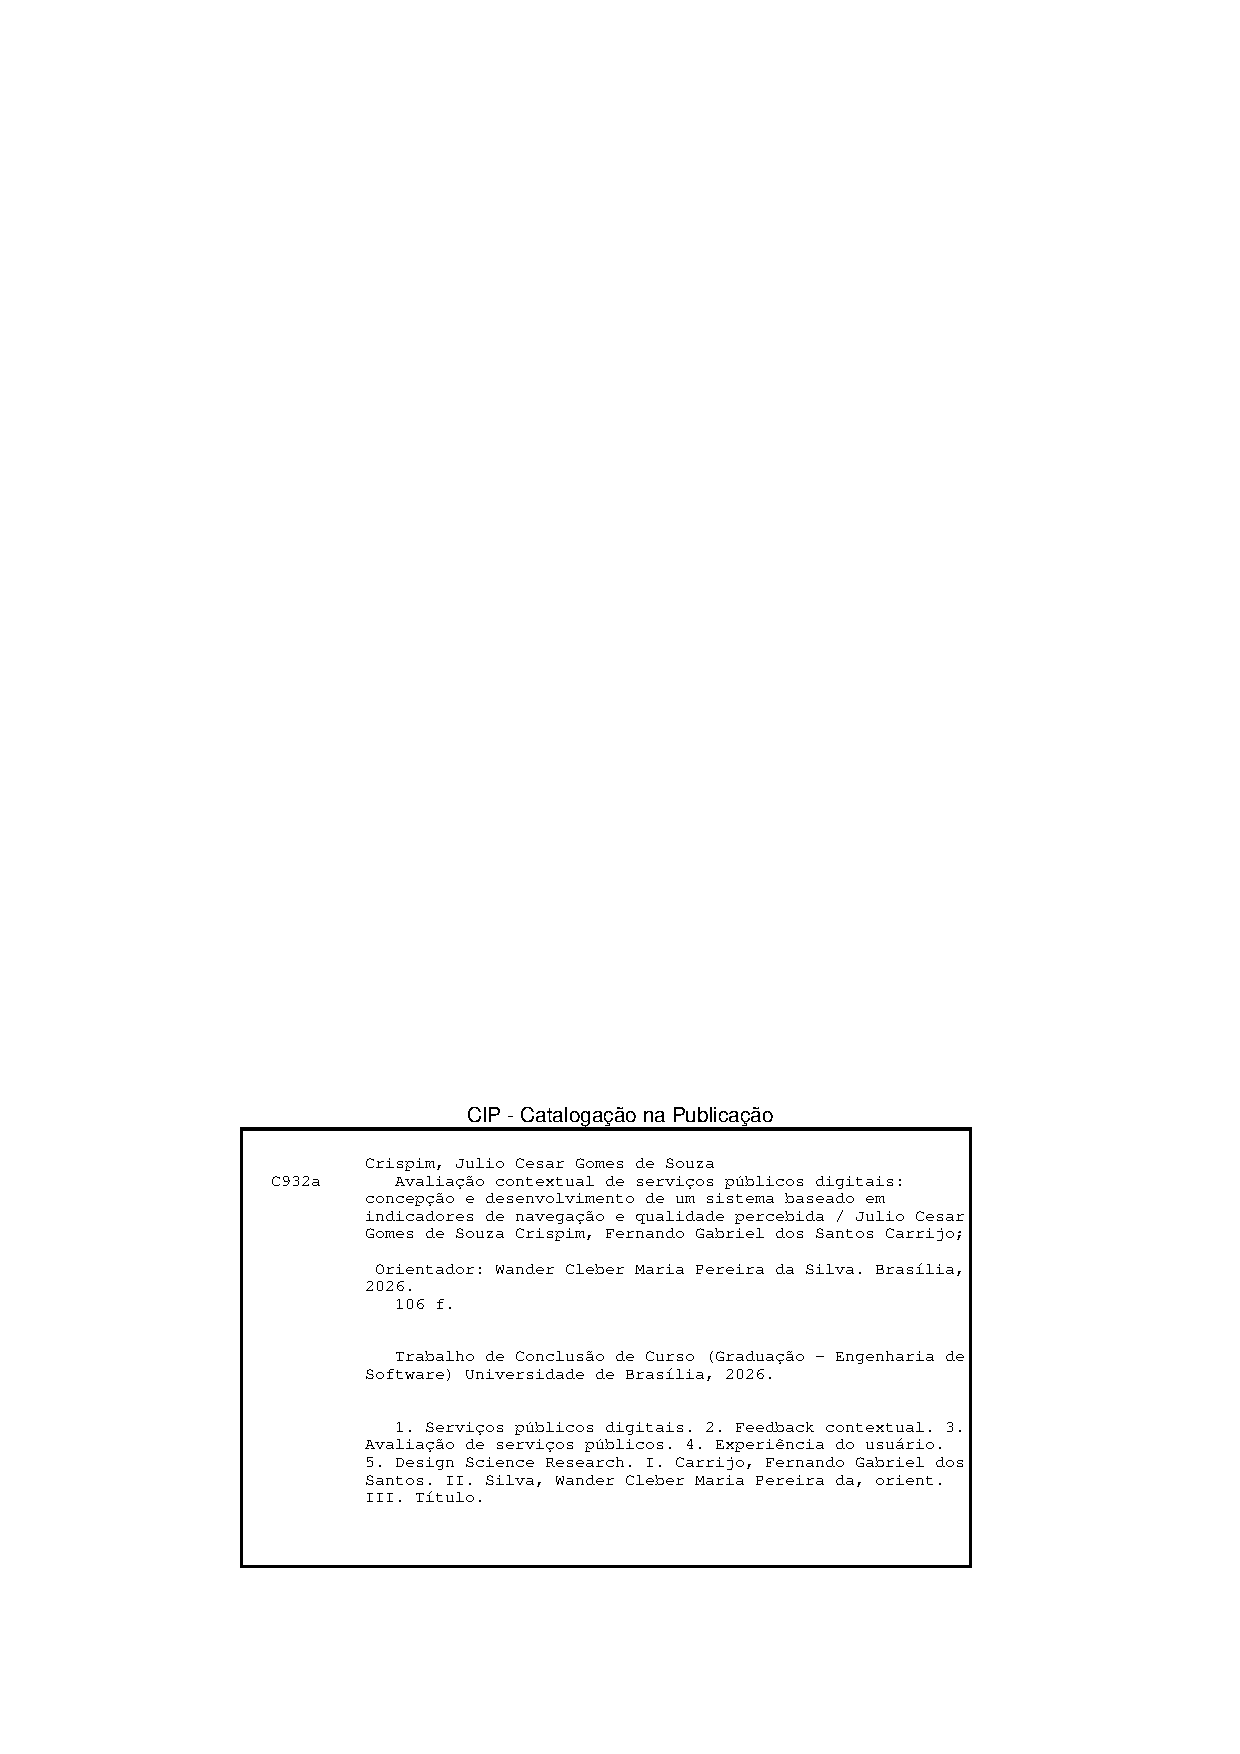
\includepdf[pages=1,fitpaper=true,pagecommand={\thispagestyle{empty}}]{pretextuais/ficha-catalografica.pdf}

\begin{folhadeaprovacao}

  \begin{center}
    {\ABNTEXchapterfont\large\imprimirautor}

    \vspace*{\fill}\vspace*{\fill}
    {\ABNTEXchapterfont\bfseries\Large\imprimirtitulo}
    \vspace*{\fill}
    
    \hspace{.45\textwidth}
    \begin{minipage}{.5\textwidth}
        \imprimirpreambulo
    \end{minipage}%
    \vspace*{\fill}
   \end{center}
    
   Trabalho submetido à avaliação. Data de aprovação: \underline{\hspace{2.5cm}}.

   \assinatura{\textbf{\imprimirorientador} \\ Orientador} 
   \assinatura{\textbf{\imprimirmembroconvidadoum}\strut \\ Convidado 1}
   \assinatura{\textbf{\imprimirmembroconvidadodois}\strut \\ Convidado 2}
      
   \begin{center}
    \vspace*{0.5cm}
    {\large\imprimirlocal}
    \par
    {\large\imprimirdata}
    \vspace*{1cm}
  \end{center}
  
\end{folhadeaprovacao}

% Gerado a partir de docs/tcc.md por scripts/sincronizar_tcc.py.
\begin{resumo}
% Gerado a partir de docs/tcc.md por scripts/sincronizar_tcc.py.
Este trabalho apresenta a concepção e o desenvolvimento inicial de um sistema de avaliação contextual de serviços públicos digitais. O problema investigado é a dificuldade de relacionar avaliações declaradas pelo cidadão ao contexto de navegação em que são solicitadas. O percurso combinou revisão bibliográfica e normativa, Lean Inception e prototipação incremental, organizados pelas atividades da Design Science Research. Foi implementado um protótipo local em Python, com API, páginas simuladas, regras operacionais sobre cliques e duração informada, formulário de feedback e painel administrativo. A telemetria fornece indícios comportamentais, sem medir qualidade percebida. A versão funcional atual registra satisfação por estrelas, atributos declarados e facilidade percebida por um item CES opcional de 1 a 7. Os itens atuais de satisfação e CES foram definidos após o estudo de interface e ainda não foram avaliados com participantes. Separadamente da implementação funcional, oito participantes avaliaram fluxos de interface no Figma, com registro automático de cliques e tempos pelo Useberry e questionário pós-sessão. Quatro participantes realizaram cada fluxo, com alocação auxiliada por inteligência artificial (IA), descrita como sorteio sem registro auditável, e com popup de redirecionamento presente em ambos. Os resultados descrevem conclusão de tarefa, facilidade percebida e relatos pós-sessão. Não comprovam maior participação, maior especificidade dos comentários do formulário, funcionamento dos gatilhos da API ou superioridade do fluxo contextual. A contribuição investigativa está na formulação de uma hipótese comparativa e na distinção entre evidências comportamentais e declaradas; a contribuição tecnológica está na implementação que permite relacioná-las. Foram especificados requisitos, rastreabilidade, critérios de qualidade e protocolos prospectivos para cidadãos, gestores e especialistas. A continuidade exige executar esses protocolos e calibrar as regras antes de uso real.

\vspace{\onelineskip}
\noindent \textbf{Palavras-chave:} serviços públicos digitais; feedback contextual; avaliação de serviços; experiência do usuário; Design Science Research.
\end{resumo}

% Gerado a partir de docs/tcc.md por scripts/sincronizar_tcc.py.
\begin{otherlanguage*}{english}
\begin{resumo}[Abstract]
% Gerado a partir de docs/tcc.md por scripts/sincronizar_tcc.py.
This work presents the design and initial development of a contextual evaluation system for digital public services. The research problem concerns linking citizens\textquotesingle{} declared evaluations to the navigation context in which feedback is requested. The work combined bibliographic and regulatory review, Lean Inception, and incremental prototyping, drawing on Design Science Research. A local Python prototype was implemented with an API, simulated pages, operational rules based on clicks and reported duration, a feedback form, and an administrative dashboard. Telemetry provides behavioral indications and does not measure perceived quality. Stars and attributes capture declared judgments; this version retains NPS as an auxiliary recommendation question whose interpretation in public services has not been validated. Separately from the functional implementation, eight participants evaluated interface flows in Figma, with automatic click and time records collected through Useberry and a post-session questionnaire. Four participants performed each flow, with artificial-intelligence-assisted allocation described as a draw without an auditable record, and with a redirect popup present in both flows. The results describe task completion, perceived ease, and post-session reports. They do not establish greater participation, more specific feedback-form comments, correct API-trigger behavior, or superiority of contextual feedback. The investigative contribution is the comparative hypothesis and the distinction between behavioral and declared evidence; the technological contribution is the implementation that can connect them. Further work requires operational measures, a documented protocol, and rule calibration before deployment.

\vspace{\onelineskip}
\noindent \textbf{Keywords:} digital public services. contextual feedback. service evaluation. user experience. Design Science Research.
\end{resumo}
\end{otherlanguage*}

\pdfbookmark[0]{\listfigurename}{lof}
\listoffigures*
\cleardoublepage
\pdfbookmark[0]{Lista de quadros}{loq}
\listofquadros
\cleardoublepage
\pdfbookmark[0]{\listtablename}{lot}
\listoftables*
\cleardoublepage

\pdfbookmark[0]{Lista de apêndices}{listaapendices}
\chapter*{Lista de apêndices}

\begin{description}
    \item[Apêndice A] Síntese da Lean Inception.
    \item[Apêndice B] Fluxo conceitual do avaliador de serviços públicos.
    \item[Apêndice C] Endpoints e indicadores do protótipo.
    \item[Apêndice D] Protocolo proposto para walkthrough externo.
    \item[Apêndice E] Modelo do TCLE utilizado.
    \item[Apêndice F] Questionário pós-sessão.
    \item[Apêndice G] Dados brutos anonimizados da avaliação com participantes.
\end{description}

\cleardoublepage

% Gerado a partir de docs/tcc.md por scripts/sincronizar_tcc.py.
\begin{siglas}
\item[API] Application Programming Interface
\item[BRASP] Modelo Brasileiro de Avaliação de Serviços Públicos
\item[CEP] Comitê de Ética em Pesquisa
\item[CES] Customer Effort Score
\item[CSAT] Customer Satisfaction Score
\item[CSS] Cascading Style Sheets
\item[DSR] Design Science Research
\item[E-RecS-QUAL] Electronic Recovery Service Quality
\item[E-S-QUAL] Electronic Service Quality
\item[ESM] Experience Sampling Method
\item[FCTE] Faculdade de Ciências e Tecnologias em Engenharia
\item[HTML] HyperText Markup Language
\item[HTTP] Hypertext Transfer Protocol
\item[IA] Inteligência artificial
\item[IEC] International Electrotechnical Commission
\item[IPC NSW] Information and Privacy Commission New South Wales
\item[IRPF] Imposto sobre a Renda da Pessoa Física
\item[ISO] International Organization for Standardization
\item[JSON] JavaScript Object Notation
\item[LGPD] Lei Geral de Proteção de Dados Pessoais
\item[MVP] Minimum Viable Product
\item[PPA] Plano Plurianual
\item[RF] Requisito funcional
\item[RN] Regra de negócio
\item[RNF] Requisito não funcional
\item[SERVQUAL] Service Quality
\item[SQuaRE] Systems and software Quality Requirements and Evaluation
\item[TCC] Trabalho de Conclusão de Curso
\item[TCLE] Termo de Consentimento Livre e Esclarecido
\item[TIC] Tecnologias de Informação e Comunicação
\item[TLS] Transport Layer Security
\item[UnB] Universidade de Brasília
\item[UX] User Experience
\item[W3C] World Wide Web Consortium
\item[WCAG] Web Content Accessibility Guidelines
\end{siglas}

\input{fixos/indiceAutomatico}

\textual

% Gerado a partir de docs/tcc.md por scripts/sincronizar_tcc.py.
\chapter{Introdução}\label{sec:1}

\section{Contextualização}\label{sec:1-1}

Nas últimas décadas, a relação entre Estado e cidadão passou por uma mudança estrutural: atividades que antes dependiam de balcões presenciais, deslocamentos e atendimento físico foram progressivamente incorporadas a portais, aplicações e fluxos digitais. A plataforma GOV.BR simboliza esse movimento ao concentrar a oferta digital de serviços federais e ao reforçar a ideia de que governo digital não é apenas troca de canal, mas reorganização da forma como o cidadão encontra, solicita, acompanha e avalia serviços públicos.

Os serviços públicos compõem uma das formas mais diretas dessa relação. Solicitar um documento, consultar uma situação cadastral, acompanhar um benefício, registrar uma demanda ou acessar uma política pública são situações em que a experiência do usuário influencia a qualidade percebida da administração pública. A digitalização ampliou o alcance e a velocidade desses atendimentos, mas também deslocou parte das dificuldades para a própria navegação: localizar o serviço correto, entender a linguagem institucional, preencher etapas intermediárias e perceber se a solicitação realmente avançou.

A escala dessa transição aparece de forma clara em experiências recentes de participação digital. O Plano Plurianual (PPA) Participativo 2024-2027, por exemplo, mobilizou mais de 1,5 milhão de participantes e superou 4 milhões de acessos na plataforma Brasil Participativo, demonstrando a capacidade de mobilização do ambiente digital. Ao mesmo tempo, a experiência registrou barreiras como problemas de conectividade, dificuldade de uso, fluxos de cadastro complexos e necessidade de melhor retorno ao cidadão sobre sua contribuição \cite{brasilMgi2024ppaParticipativo}. Esse contraste reforça a importância de avaliar não apenas se o serviço existe em formato digital, mas como ele é percebido e utilizado durante a jornada.

No Brasil, a avaliação dos serviços públicos possui base legal e gerencial. A Lei n\textsuperscript{o} 13.460/2017 trata da participação, proteção e defesa dos usuários de serviços públicos e prevê que os resultados de avaliação subsidiem a reorientação e o ajuste da prestação estatal \cite{brasil2017lei13460}. O Decreto n\textsuperscript{o} 9.094/2017 institui a Carta de Serviços ao Usuário e reforça a simplificação do atendimento \cite{brasil2017decreto9094}. A Lei n\textsuperscript{o} 14.129/2021 associa governo digital, eficiência pública, desburocratização e participação do cidadão \cite{brasil2021lei14129}. Como referência histórica, o Decreto n\textsuperscript{o} 11.260/2022 tratou da elaboração da Estratégia Nacional de Governo Digital e da prorrogação da estratégia anterior; foi revogado em 2024 e não é apresentado como norma vigente \cite{brasil2022decreto11260}.

A avaliação da experiência digital, porém, não depende apenas de perguntar ao usuário se ele ficou satisfeito ao final do atendimento. Em serviços digitais, excesso de cliques, permanência por tempo acima do esperado, retorno repetido a páginas anteriores e abandono antes da conclusão constituem evidências comportamentais de possível dificuldade. Esses sinais não medem qualidade percebida e não autorizam, isoladamente, concluir que a experiência foi ruim. Quando coletados com finalidade clara e com cuidado em relação à privacidade, eles ajudam a localizar pontos da jornada que devem ser investigados e confrontados com a percepção declarada pelo usuário \cite{deloneMclean2003,govuk2021completionRate,brasil2018lgpd}.

A proposta é relacionar evidências comportamentais e declaradas sem tratá-las como equivalentes. A implementação Python registra cliques em elementos instrumentados, página, serviço e informações do evento; recebe também uma duração informada à API, demonstrada por envio simulado de 120 segundos, sem cronômetro automático no cliente. Regras operacionais podem gerar uma sugestão de redirecionamento ou disponibilizar um convite. Estrelas, atributos, CES e comentários permitem examinar julgamentos declarados sobre satisfação, aspectos do serviço, facilidade percebida e contexto qualitativo, respectivamente. Esses indicadores têm interpretações distintas e não formam um escore único de qualidade. O estudo com participantes ocorreu separadamente, em interfaces no Figma, com cliques e tempos registrados automaticamente pelo Useberry.

A proposta adota uma interface curta de avaliação e mantém uma implementação local de registro de eventos e feedback. A visualização administrativa disponível apresenta alertas, contagens por serviço e médias de respostas. O painel apresenta frequência de atributos, sessões distintas alertadas e ações com acompanhamento. Taxa de resposta por fluxo ainda depende de instrumentação A/B e de exposição. A Lean Inception orientou a delimitação do produto e do MVP, cujas funcionalidades foram implementadas parcialmente \cite{caroli2018leanInception,fowler2022leanInception}.

\section{Problema de Pesquisa}\label{sec:1-2}

A questão investigada é como relacionar a avaliação declarada pelo cidadão ao contexto de navegação em que ela é solicitada. Quando a coleta fica restrita ao final da jornada, pode deixar de registrar detalhes de uma etapa anterior ou de um fluxo interrompido. Essa possibilidade motiva o estudo do momento do convite, sem pressupor que a coleta contextual produza resultados superiores. Indicadores só se tornam úteis à gestão quando seu contexto e suas limitações são considerados \cite{govuk2021usingData,deloneMclean2003}.

Modelos oficiais e instrumentos consolidados de avaliação de serviços públicos contribuem para a mensuração da satisfação e da qualidade percebida. Ainda assim, permanecem desafios relacionados à baixa adesão, ao esforço exigido do usuário e à transformação das respostas em informação acionável para o gestor. Avaliações longas podem reduzir a participação; avaliações curtas podem gerar indicadores pouco explicativos; dados de navegação sem interpretação podem produzir apenas registros técnicos sem valor gerencial. A literatura científica mostra que taxas de resposta variam entre modos de coleta e populações, e que a formulação e o contexto das perguntas influenciam os relatos dos respondentes \cite{shihFan2008responseRates,manfreda2008webSurveys,schwarz1999selfReports}. Esses estudos justificam examinar adesão e desenho da coleta, mas não demonstram superioridade do feedback contextual em serviços públicos digitais. O uso dos registros para melhoria também exige interpretação dos dados de desempenho e atenção à relação entre qualidade do sistema, satisfação e benefícios \cite{govuk2021usingData,deloneMclean2003}.

Este trabalho parte da seguinte questão de pesquisa: como propor e prototipar um avaliador de serviços públicos digitais que identifique sinais de possível dificuldade na navegação, colete feedback contextual de baixo esforço e organize informações úteis para a melhoria dos serviços avaliados?

A comparação entre convite contextual e formulário final foi organizada nas hipóteses H1 e H2, formuladas na seção \ref{sec:3-6-1}. Elas tratam, respectivamente, de participação e especificidade dos comentários do formulário. Os resultados disponíveis são observações exploratórias de interface e não testam essas hipóteses.

\section{Objetivo Geral}\label{sec:1-3}

Propor e desenvolver um protótipo inicial de avaliador de serviços públicos digitais capaz de registrar sinais de possível dificuldade na navegação, coletar feedback contextual estruturado, comparar esse fluxo com uma avaliação estática e apresentar indicadores administrativos que apoiem a melhoria contínua dos serviços.

\section{Objetivos Específicos}\label{sec:1-4}

Para alcançar o objetivo geral, foram definidos os seguintes objetivos específicos:

\begin{itemize}
\item
  levantar fundamentos legais, técnicos e teóricos sobre avaliação de serviços públicos, qualidade percebida, usabilidade, governo digital e Lean Inception;
\item
  definir, por meio de Lean Inception, o fluxo de detecção de possível dificuldade, sugestão de redirecionamento e coleta de feedback;
\item
  construir um protótipo funcional com API, páginas simuladas de serviço público, feedback contextual, formulário estático comparativo e visualização administrativa;
\item
  estruturar os dados e indicadores necessários para apoiar a análise de cliques, tempo de navegação, taxa de resposta, satisfação por estrelas, esforço percebido pelo CES e pontos recorrentes de melhoria.
\end{itemize}

A estrutura dos objetivos combina a fundamentação legal e técnica da avaliação de serviços públicos com práticas de definição de MVP e prototipação de software \cite{brasil2017lei13460,brasil2021lei14129,caroli2018leanInception,Sommerville2011}.

\section{Justificativa}\label{sec:1-5}

Mecanismos digitais de avaliação podem fortalecer a participação do usuário na melhoria dos serviços públicos. Os materiais da Enap destacam que a avaliação centrada no cidadão desloca o foco das ferramentas tecnológicas para as necessidades, demandas e satisfação dos usuários \cite{limaPereira2020modulo1}. Também indicam que avaliações devem alimentar ciclos de melhoria, permitindo identificar problemas recorrentes, atributos críticos e prioridades de intervenção \cite{limaPereira2020modulo4}.

A proposta é relevante porque muitos usuários já conhecem avaliações simples por estrelas, motivos e comentários. Uma solução pública pode aproveitar essa familiaridade para reduzir o esforço de resposta, desde que use os dados para finalidades compatíveis com o interesse público. Além disso, a combinação entre eventos de navegação e feedback declarado permite que o gestor observe tanto o que o usuário informou quanto o que ocorreu durante a jornada digital.

Do ponto de vista investigativo, o trabalho formula hipóteses sobre o momento da coleta e distingue indícios comportamentais de percepção declarada. A organização conceitual é explicitada no Quadro \ref{tab:construtos-indicadores-dados}, com dados, origem e limites de interpretação; sua validade ainda depende de avaliação empírica. Do ponto de vista tecnológico, a contribuição é a implementação de API, telas, regras explícitas e painel que permitem associar contexto de navegação e relato do cidadão. As configurações possuem versões e histórico local, o que permite inspecionar alterações, sem equivaler a auditoria independente \cite{deloneMclean2003,hevner2004designscience,Sommerville2011}.

\section{Escopo Inicial}\label{sec:1-6}

O escopo inicial concentra-se na proposta e prototipação de uma solução. O trabalho não pretende implantar um sistema em ambiente governamental real, nem substituir instrumentos oficiais de avaliação já existentes. A solução é complementar e exploratória: simula páginas de serviço público, registra eventos de navegação, aplica regras configuráveis de acionamento por sinais de possível dificuldade, abre uma coleta simples de feedback, inclui um formulário reutilizável e apresenta dados administrativos agregados. A comparação entre formulário final e convite contextual pertence ao desenho de interface no Figma; a aplicação Python ainda não distingue os grupos nem registra a exposição. Essa delimitação segue a lógica de prototipação como forma de reduzir incertezas antes de uma solução definitiva e mantém cuidado com minimização de dados pessoais \cite{Sommerville2011,brasil2018lgpd}.

A avaliação desta etapa reúne procedimentos distintos: inspeção funcional e heurística interna/preliminar relatada pelos autores, e sessões exploratórias de interface com oito participantes no Figma, instrumentadas pelo Useberry. Essas sessões não constituem teste de integração ou execução da API Python. Os resultados são descritivos, sem generalização estatística ou validação em contexto real de prestação de serviço público. Integração com portais governamentais, calibração e estudo comparativo permanecem etapas futuras.

% Gerado a partir de docs/tcc.md por scripts/sincronizar_tcc.py.
\chapter{Referencial Teórico}\label{referencial-teuxf3rico}

Avaliar um serviço público digital exige olhar para mais do que a tela final de confirmação. A experiência do cidadão começa quando ele tenta entender onde está o serviço, continua nos caminhos que percorre e termina apenas quando a demanda é resolvida ou abandonada. Por isso, este capítulo reúne os fundamentos que sustentam a proposta do avaliador: conceitos de serviço público, satisfação, qualidade percebida, usabilidade, modelos brasileiros de avaliação e sinais de possível dificuldade observáveis durante a navegação.

O capítulo também parte de uma tradição anterior à digitalização dos serviços: os modelos clássicos de qualidade em serviços. Essa base é importante porque mostra que a percepção do usuário sempre dependeu da comparação entre o que ele esperava receber e o que efetivamente experimentou. No ambiente público digital, essa comparação passa a envolver, além do resultado do serviço, a clareza da informação, a confiança no canal, a facilidade de navegação, o esforço exigido e a capacidade do órgão de responder ao problema identificado \cite{gronroos1984service,parasuraman1988servqual,deloneMclean2003}.

\section{Serviços e Serviços Públicos}\label{serviuxe7os-e-serviuxe7os-puxfablicos}

Serviços diferenciam-se de produtos porque são mais intangíveis, ocorrem como séries de atividades, envolvem algum grau de interação com o usuário e, em muitos casos, são produzidos e consumidos simultaneamente. Essa característica torna a avaliação de serviços mais dependente da experiência vivida pelo usuário, e não apenas de propriedades observáveis de um bem material \cite{gronroos1984service,limaPereira2020modulo1}.

No setor público, o serviço é parte do relacionamento entre cidadão e Estado. Ele pode envolver uma entrega individualizada, como a emissão de um documento, ou uma entrega de interesse coletivo, como segurança, educação, saúde e infraestrutura. Por isso, a avaliação de serviços públicos possui uma dimensão adicional: além de medir satisfação ou qualidade, ela se conecta ao exercício da cidadania, à prestação de contas e ao aperfeiçoamento da administração pública \cite{brasil2017lei13460,brasil2021lei14129,limaPereira2020modulo1}.

Com a digitalização, muitos serviços passaram a ser acessados por portais, aplicativos e sistemas integrados. Essa mudança amplia o alcance da prestação pública, mas também cria novas exigências de usabilidade, clareza, confiabilidade e disponibilidade. A usabilidade pode ser entendida como resultado de uso associado à efetividade, eficiência e satisfação em um contexto definido \cite{iso9241112018}. O usuário não avalia apenas o resultado final do serviço; ele também avalia o caminho percorrido, a linguagem utilizada, o esforço exigido, a facilidade de navegação e a capacidade do canal digital de resolver sua demanda.

\subsection{Serviço digital, interação e resultado pretendido}\label{serviuxe7o-digital-interauxe7uxe3o-e-resultado-pretendido}

Neste trabalho, serviço público digital é o arranjo de informações, procedimentos, pessoas, regras e recursos tecnológicos pelo qual o cidadão busca um resultado de interesse público. O portal é um canal desse arranjo. Encontrar uma página ou concluir uma interação não significa necessariamente obter o documento, benefício ou solução pretendida. A orientação institucional de resolver o problema completo do usuário ajuda a delimitar essa diferença \cite{govuk2026wholeProblem}.

A avaliação distingue quatro objetos: \textbf{qualidade do software}, relativa às propriedades da aplicação e da API; \textbf{qualidade da interação}, relativa às condições e resultados do uso da interface; \textbf{qualidade percebida do serviço}, relativa ao julgamento declarado sobre aspectos da prestação; e \textbf{efetividade do serviço}, relativa ao alcance do resultado pretendido. A primeira é tratada pelo modelo de qualidade de produto ISO/IEC 25010:2023; a usabilidade em contexto considera efetividade, eficiência e satisfação conforme ISO 9241-11; os atributos de serviço e a conclusão real exigem evidências próprias \cite{iso250102023,iso9241112018}.

Por exemplo, uma API pode aceitar e armazenar corretamente uma avaliação sem que o cidadão tenha conseguido declarar o imposto. Uma interface pode ser fácil de navegar, mas conduzir à consulta quando a necessidade era declarar. Uma nota favorável não prova que a obrigação foi cumprida. A conclusão de tarefa registrada no Figma é efetividade da tarefa simulada, não entrega de um serviço público real. O avaliador apoia investigação sobre a jornada; não executa nem certifica essa entrega.

\section{Avaliação de Serviços}\label{avaliauxe7uxe3o-de-serviuxe7os}

A avaliação de serviços pode ser entendida como uma investigação qualitativa ou quantitativa sobre a qualidade do serviço e a satisfação do usuário, considerando a relação entre expectativa e experiência concreta \cite{limaPereira2020modulo1}. Em outras palavras, avaliar um serviço significa observar se a entrega realizada corresponde ao que o usuário precisava, esperava ou considerava adequado. Modelos clássicos de qualidade de serviço indicam que a percepção do usuário é formada por lacunas entre o serviço esperado e o serviço recebido. O modelo de qualidade percebida de \citeonline{gronroos1984service} e o modelo SERVQUAL de \citeonline{parasuraman1988servqual} consolidaram a ideia de que qualidade em serviços depende de fatores como confiabilidade, responsividade, segurança, empatia e aspectos tangíveis. Embora esses modelos tenham origem no setor privado, eles influenciaram diversas iniciativas posteriores de avaliação de serviços públicos e serviços digitais.

No SERVQUAL, essas dimensões aparecem como tangibilidade, confiabilidade, responsividade, garantia e empatia. A contribuição central do modelo é tratar a qualidade percebida como diferença entre expectativa prévia e percepção após a experiência. Para serviços públicos, entretanto, essa leitura exige adaptação: o cidadão geralmente não escolhe entre prestadores concorrentes e muitas vezes depende daquele serviço para exercer um direito, cumprir uma obrigação ou acessar um benefício. Assim, a expectativa não é formada apenas por comparação de mercado, mas também por experiências anteriores com o Estado, comunicação institucional, relatos de outros usuários e, mais recentemente, pela comparação com serviços digitais privados que oferecem interfaces mais rápidas e responsivas \cite{parasuraman1988servqual,limaPereira2020modulo2}.

Nos serviços digitais, a avaliação passou a incorporar fatores ligados ao uso de sistemas de informação, como qualidade do sistema, qualidade da informação, qualidade do serviço, intenção de uso, satisfação do usuário e benefícios percebidos. Os materiais da Enap destacam que, à medida que cidadãos passaram a interagir com sistemas governamentais digitais, tornou-se necessário adotar modelos capazes de avaliar não apenas páginas ou portais, mas a experiência do usuário ao longo da prestação do serviço \cite{limaPereira2020modulo2,deloneMclean2003,pedrosa2019qualidadeGovbr}.

\section{Satisfação e Qualidade Percebida}\label{satisfauxe7uxe3o-e-qualidade-percebida}

Satisfação e qualidade percebida são conceitos próximos, mas não idênticos. A satisfação costuma expressar um julgamento global do usuário após consumir o serviço, enquanto a qualidade percebida pode ser decomposta em atributos mais específicos da experiência, como rapidez, clareza das informações, atendimento, esforço, confiabilidade e facilidade de uso. Para \citeonline{oliver2014satisfaction}, a satisfação está relacionada ao julgamento do usuário sobre o grau em que uma experiência atendeu ou não suas expectativas.

No contexto público, a distinção entre satisfação e qualidade percebida é importante porque uma nota geral, sozinha, nem sempre indica o que deve ser melhorado. Um usuário pode avaliar mal um serviço por demora, linguagem confusa, instabilidade do sistema, falta de atendimento ou excesso de etapas. Portanto, um avaliador de serviços públicos precisa combinar uma avaliação simples, como nota ou estrelas, com mecanismos que ajudem a qualificar o motivo da avaliação.

Essa lógica aparece na evolução dos instrumentos brasileiros de avaliação. O BRASP considera a qualidade percebida como um elemento central para compreender a experiência do usuário e apoiar o aprimoramento dos serviços \cite{silva2019brasp}. A proposta de modelo unificado busca integrar qualidade técnica, qualidade percebida, efetividade e satisfação, reduzindo o custo de resposta para o cidadão e tornando os resultados mais úteis para a gestão \cite{silva2022modeloUnificado}.

\section{Qualidade de Serviços Eletrônicos e Governo Eletrônico: E-S-QUAL, E-RecS-QUAL e e-GovQual}\label{qualidade-de-serviuxe7os-eletruxf4nicos-e-governo-eletruxf4nico-e-s-qual-e-recs-qual-e-e-govqual}

A passagem dos modelos gerais para os serviços eletrônicos exige considerar a prestação mediada por sistemas. \citeonline{parasuraman2005esqual} desenvolveram E-S-QUAL para sites de compras, com 22 itens e quatro dimensões: eficiência, cumprimento da prestação, disponibilidade do sistema e privacidade. E-RecS-QUAL trata situações não rotineiras e recuperação do serviço, com 11 itens em responsividade, compensação e contato. São escalas distintas; uma avaliação de recuperação pressupõe que tenha ocorrido uma situação pertinente.

A aplicação ao presente artefato é uma decisão de análise, não a aplicação integral dessas escalas. Eficiência motiva examinar caminhos e facilidade declarada; disponibilidade motiva testes técnicos; cumprimento motiva separar navegação de resultado; privacidade motiva requisitos de coleta. Na recuperação, responsividade e contato orientam investigar suporte e retorno ao cidadão. Compensação depende da natureza do serviço e de seu enquadramento institucional; não é inferida dos cliques ou de um comentário.

Os seis atributos do formulário não reproduzem os itens de E-S-QUAL/E-RecS-QUAL nem geram seus escores. O CES é outro indicador, e não uma dimensão substituta dessas escalas. Para serviços públicos, a interpretação precisa considerar direitos, obrigações, continuidade entre canais e ausência de escolha de prestador. Essa delimitação conduz aos modelos brasileiros apresentados nas seções seguintes, preservando a progressão qualidade de serviços \ensuremath{\rightarrow} serviços eletrônicos \ensuremath{\rightarrow} serviços públicos digitais \ensuremath{\rightarrow} BRASP e modelos nacionais.

No domínio governamental, \citeonline{papadomichelaki2012egovqual} desenvolveram e-GovQual para sites públicos nos quais o cidadão procura informação ou serviço. A escala final reúne 21 itens em confiabilidade, eficiência, suporte ao cidadão e confiança. Esse modelo oferece o elo entre qualidade eletrônica e prestação pública digital, sem reduzir a avaliação à transação comercial.

Neste trabalho, e-GovQual orienta examinar a consistência da prestação, a facilidade de acesso à informação, os caminhos de suporte e a confiança na coleta. São relações conceituais de projeto: o formulário não reproduz seus 21 itens, e os seis atributos não geram um escore e-GovQual. A validação relatada por Papadomichelaki e Mentzas não se transfere ao CES adaptado nem a este protótipo. O modelo internacional antecede, nesta progressão, os instrumentos brasileiros e o BRASP discutidos a seguir.

\section{Avaliação de Serviços Públicos no Brasil}\label{avaliauxe7uxe3o-de-serviuxe7os-puxfablicos-no-brasil}

A avaliação de serviços públicos no Brasil possui base normativa e base técnica. Do ponto de vista normativo, a Lei n\textsuperscript{o} 13.460/2017 estabelece direitos dos usuários e prevê que os resultados de avaliação subsidiem a reorientação dos serviços \cite{brasil2017lei13460}. O Decreto n\textsuperscript{o} 9.094/2017 institui a Carta de Serviços ao Usuário e reforça o uso de ferramenta de pesquisa de satisfação no governo federal \cite{brasil2017decreto9094}. A Lei n\textsuperscript{o} 14.129/2021 relaciona o governo digital à eficiência pública, à desburocratização e à participação do cidadão \cite{brasil2021lei14129}.

A partir desse conjunto normativo, a avaliação deixa de ser apenas uma prática gerencial desejável e passa a compor o próprio modo de prestação dos serviços públicos digitais. A Lei de Acesso à Informação reforça a transparência como base para acompanhamento social; a Lei n\textsuperscript{o} 13.460/2017 vincula avaliação à proteção do usuário; a Lei do Governo Digital incorpora canais digitais de participação; e normas infralegais detalham instrumentos de simplificação, monitoramento e avaliação de satisfação. O Quadro \ref{tab:marcos-legais-avaliacao} resume os marcos mais relevantes para este trabalho.

\begingroup\footnotesize\SingleSpacing
\setlength{\tabcolsep}{4pt}
\setlength{\LTpre}{.6\baselineskip}
\setlength{\LTpost}{.4\baselineskip}
\setlength{\LTcapwidth}{\textwidth}

\begin{TCCquadro}
\begin{longtable}[]{@{}
  >{\RaggedRight\arraybackslash}p{(\linewidth - 4\tabcolsep) * \real{0.2800}}
  >{\RaggedRight\arraybackslash}p{(\linewidth - 4\tabcolsep) * \real{0.1200}}
  >{\RaggedRight\arraybackslash}p{(\linewidth - 4\tabcolsep) * \real{0.6000}}@{}}
\caption[]{\TCCquadroentry{Marcos legais nacionais sobre avaliação de serviços públicos digitais}Marcos legais nacionais sobre avaliação de serviços públicos digitais}\label{tab:marcos-legais-avaliacao}\tabularnewline
\toprule\noalign{}
\begin{minipage}[b]{\linewidth}\raggedright
\textbf{Instrumento}
\end{minipage} & \begin{minipage}[b]{\linewidth}\raggedright
\textbf{Ano}
\end{minipage} & \begin{minipage}[b]{\linewidth}\raggedright
\textbf{Principais disposições relevantes}
\end{minipage} \\
\midrule\noalign{}
\endfirsthead
\caption[]{Marcos legais nacionais sobre avaliação de serviços públicos digitais (continuação)}\tabularnewline
\toprule\noalign{}
\begin{minipage}[b]{\linewidth}\raggedright
\textbf{Instrumento}
\end{minipage} & \begin{minipage}[b]{\linewidth}\raggedright
\textbf{Ano}
\end{minipage} & \begin{minipage}[b]{\linewidth}\raggedright
\textbf{Principais disposições relevantes}
\end{minipage} \\
\midrule\noalign{}
\endhead
\bottomrule\noalign{}
\endlastfoot
Lei n\textsuperscript{o} 12.527 (LAI) \cite{brasil2011lei12527} & 2011 & Transparência ativa e passiva; base para acesso a informações públicas e dados sobre desempenho de serviços. \\
Lei n\textsuperscript{o} 13.460 \cite{brasil2017lei13460} & 2017 & Direitos do usuário, participação na avaliação dos serviços e uso dos resultados para reorientação da prestação pública. \\
Decreto n\textsuperscript{o} 9.094 \cite{brasil2017decreto9094} & 2017 & Simplificação do atendimento, Carta de Serviços ao Usuário e racionalização de exigências feitas ao cidadão. \\
Lei n\textsuperscript{o} 14.129 \cite{brasil2021lei14129} & 2021 & Governo digital, eficiência pública, desburocratização, canais digitais de participação e melhoria da prestação estatal. \\
Decreto n\textsuperscript{o} 11.260 \cite{brasil2022decreto11260} & 2022 & Referência histórica sobre elaboração da estratégia e prorrogação da anterior; revogado em 2024, sem caráter de norma vigente neste trabalho. \\
Portaria SGD/ME n\textsuperscript{o} 548 \cite{brasil2022portaria548} & 2022 & Avaliação de satisfação dos usuários e padrões de qualidade para serviços públicos digitais. \\
\end{longtable}
\end{TCCquadro}

\endgroup

Fonte: elaborada pelos autores com base na legislação federal brasileira.

Do ponto de vista técnico, relatórios produzidos no âmbito da Universidade de Brasília, da Secretaria de Governo Digital e de instituições parceiras apresentam modelos voltados à mensuração da qualidade de serviços públicos digitais. A proposta Qualidade Gov.br organiza a avaliação em dimensões ligadas à consistência digital e à experiência do usuário, reconhecendo que a qualidade de um serviço digital depende tanto dos requisitos técnicos quanto da jornada do cidadão \cite{pedrosa2019qualidadeGovbr}. O BRASP amplia essa discussão ao considerar serviços presenciais, digitizados e parcialmente digitizados \cite{silva2019brasp}.

O avanço desses modelos demonstra que a avaliação pública precisa equilibrar rigor metodológico e simplicidade operacional. Instrumentos longos e complexos podem gerar dados ricos, mas tendem a aumentar o esforço do respondente. Por outro lado, instrumentos muito curtos podem ampliar a adesão, mas produzir dados insuficientes para orientar melhorias. Esse equilíbrio é especialmente relevante para a proposta deste TCC, que busca um avaliador simples para o cidadão e útil para a gestão.

\section{BRASP, API de Avaliação e Modelo Unificado}\label{brasp-api-de-avaliauxe7uxe3o-e-modelo-unificado}

O Modelo Brasileiro de Avaliação de Serviços Públicos (BRASP) foi desenvolvido para construir e validar instrumentos de avaliação da qualidade adaptados à realidade brasileira. O modelo considera três modalidades de prestação: serviços digitizados, serviços parcialmente digitizados e serviços presenciais \cite{silva2019brasp}. Essa diferenciação é relevante porque a experiência do usuário muda de acordo com o canal. Um serviço presencial pode depender mais de atendimento, espera e estrutura física; um serviço digital pode depender mais de facilidade de uso, clareza, disponibilidade e segurança; e um serviço híbrido pode combinar problemas de ambos os contextos.

Nos materiais da Enap, o modelo brasileiro de avaliação é apresentado como instrumento para identificar fatores relacionados à satisfação do usuário, localizar pontos críticos e gerar comparações capazes de acompanhar a evolução dos serviços. Essa leitura é coerente com o BRASP e com a proposta de modelo unificado, que organizam satisfação, qualidade percebida, qualidade técnica e efetividade como dimensões complementares de análise \cite{limaPereira2020modulo3,silva2019brasp,silva2022modeloUnificado}. A pesquisa de satisfação aparece ancorada em uma pergunta geral sobre a experiência com o serviço, enquanto a qualidade percebida é investigada por atributos que ajudam a explicar essa experiência.

A API de avaliação do governo brasileiro segue uma lógica semelhante. Segundo o relatório sobre os atributos da API, a satisfação é medida por uma estratégia simples inspirada no CSAT, com resposta por opções associadas a estrelas, e a qualidade percebida é explorada por atributos como clareza das informações, custo ou esforço para obtenção do serviço, disponibilidade, eficácia, facilidade de uso, qualidade dos canais de comunicação e tempo para obtenção do serviço \cite{silva2024atributosApi}. Essa abordagem se aproxima da proposta deste trabalho, pois combina avaliação rápida com categorização do motivo da nota.

A proposta de modelo unificado reforça essa direção ao articular quatro eixos: qualidade técnica, qualidade percebida, satisfação do usuário e efetividade \cite{silva2022modeloUnificado}. Para um avaliador de serviços públicos, esses eixos podem orientar tanto a coleta quanto a visualização de dados. A satisfação indica o julgamento geral do cidadão; a qualidade percebida explica a experiência por atributos; a qualidade técnica pode apoiar análises de disponibilidade, integração e consistência; e a efetividade aproxima a avaliação da pergunta central: o serviço resolveu a necessidade do usuário?

\section{Usabilidade, Inclusão Digital e Métricas de Experiência}\label{usabilidade-inclusuxe3o-digital-e-muxe9tricas-de-experiuxeancia}

A usabilidade em serviços públicos digitais possui impacto mais amplo do que em produtos privados. Quando uma interface privada é difícil, o usuário pode trocar de fornecedor; quando um serviço público digital é difícil, o cidadão pode perder prazo, deixar de acessar um benefício, não concluir uma obrigação ou depender de atendimento presencial. Por isso, os princípios de usabilidade precisam ser interpretados como parte do acesso efetivo ao serviço. As heurísticas de \citeonline{nielsen1994heuristic}, como visibilidade do status do sistema, correspondência entre linguagem da interface e linguagem do usuário, prevenção de erros e ajuda contextual, são diretamente relacionadas aos problemas que o avaliador busca observar durante a navegação.

A representatividade também é um ponto relevante. Serviços públicos atendem usuários com diferentes níveis de letramento digital, conectividade, idade, familiaridade com formulários e capacidade de compreender linguagem institucional. Os dados do PPA Participativo 2024-2027 indicam que participação digital em larga escala pode conviver com barreiras de uso e de retorno ao cidadão \cite{brasilMgi2024ppaParticipativo}. Da mesma forma, pesquisas sobre acesso às tecnologias de informação no Brasil mostram que o uso de serviços digitais ainda depende de condições desiguais de acesso, dispositivos e habilidades \cite{cetic2025ticDomicilios2024}. Para este TCC, isso reforça a necessidade de uma coleta de feedback simples, opcional e de baixo esforço.

O CSAT e o CES abordam julgamentos diferentes. A satisfação expressa a avaliação do cidadão sobre a experiência com a etapa do serviço; o CES aborda a facilidade ou o esforço percebido nessa interação. A proposta usa estrelas como operacionalização local de satisfação, atributos para detalhar aspectos do serviço e um item CES para facilidade percebida. Nenhum deles é obtido diretamente da telemetria. A discussão profissional de \citeonline{dixon2010effort} motiva atenção ao esforço, mas sua origem em atendimento comercial não demonstra validade em serviços públicos.

A literatura profissional de \citeonline{dixon2013effortless} desenvolve a abordagem de experiência com menor esforço no atendimento comercial. Para a formulação por concordância, a apresentação de \citeonline[slide 72]{dixon2016ces} mostra o CES 2.0 com afirmação sobre facilidade para lidar com uma questão. Esse material primário distingue a formulação posterior da referência de 2010, que não é utilizada para atribuir origem à redação ou à escala adotadas aqui. A conferência visual desse slide identifica seis opções visíveis, não sete; ele fundamenta a formulação por concordância, não o número de categorias adotado neste projeto. A frase em português, o recorte por etapa e as sete categorias são decisões de adaptação deste projeto, ainda sem validação com cidadãos.

O CES adotado usa a afirmação ``Foi fácil realizar o que eu precisava nesta etapa do serviço'', com sete categorias: 1 --- discordo totalmente; 2 --- discordo; 3 --- discordo parcialmente; 4 --- nem concordo nem discordo; 5 --- concordo parcialmente; 6 --- concordo; 7 --- concordo totalmente. A resposta é opcional. Notas maiores significam maior facilidade declarada e, nessa orientação, menor esforço percebido. Não se inverte o resultado nem se combina essa escala com medidas de outra orientação. Trata-se de adaptação ao contexto deste protótipo, não de uma tradução validada. A documentação de \citeonline{surveymonkey2026ces} é utilizada como apoio comercial complementar à descrição operacional, sem importar alegações comerciais de desempenho ou pontos de corte.

A média CES descritiva é a soma das respostas válidas dividida pelo número de respostas válidas, com apresentação conjunta da distribuição nas sete categorias e do denominador. Ausência de resposta fica nula, nunca zero; na ausência de respostas, a média fica indisponível. A média resume uma escala ordinal por convenção descritiva do protótipo e não comprova intervalos equivalentes entre categorias. Não se adotam faixas universais de ``bom'' ou ``ruim'' nem um escore geral resultante da soma de estrelas, atributos, CES e telemetria.

O item se refere à etapa vivenciada até o convite, inclusive quando a tarefa não foi concluída. A expressão ``realizar o que eu precisava'' pode, porém, ser interpretada como tarefa já concluída; o piloto de compreensão deverá verificar esse risco antes de manter a redação em convite intermediário. Portanto, facilidade declarada não comprova entrega do resultado pretendido pelo cidadão. O momento da coleta pode influenciar recordação e interpretação. Resultados sobre avaliação retrospectiva motivam investigar esse efeito, sem demonstrar a vantagem do acionamento neste cenário \cite{kahneman1993peakEnd}. O esforço para preencher o próprio formulário é outra variável e requer medida específica.

\section{Experiência do Usuário e Avaliações Inspiradas em Plataformas Digitais}\label{experiuxeancia-do-usuuxe1rio-e-avaliauxe7uxf5es-inspiradas-em-plataformas-digitais}

Plataformas digitais privadas popularizaram formas de avaliação de baixo esforço: nota de uma a cinco estrelas, comentários curtos, seleção de motivos e visualização agregada das avaliações. A referência a aplicações como plataformas de entrega deve ser entendida como inspiração de interação, e não como modelo de governança. Em uma plataforma privada, a avaliação frequentemente orienta reputação, consumo e concorrência. Em serviços públicos, ela deve orientar direitos, transparência, participação social e melhoria da entrega estatal.

Mesmo com essa diferença, a familiaridade do usuário com mecanismos simples de avaliação pode ser aproveitada. Um avaliador de serviços públicos pode reduzir barreiras de participação se oferecer uma interface direta, com poucos passos e linguagem compreensível. A nota geral permite captar a percepção imediata; os atributos permitem interpretar os motivos; e comentários opcionais podem revelar problemas não previstos pelo formulário. Essa escolha está alinhada ao design centrado no usuário, que orienta o desenvolvimento de sistemas interativos a partir das necessidades, capacidades e limitações das pessoas que irão utilizá-los \cite{iso92412102019}.

Para que a avaliação seja útil ao gestor, o sistema também precisa organizar os dados coletados. Isso envolve agrupar avaliações por serviço, período, órgão, canal e atributo; identificar itens recorrentes; apresentar médias e distribuições; e permitir comparação temporal. A literatura de melhoria de serviços reforça que as avaliações devem alimentar ciclos de melhoria contínua, funcionando como linha de base para decisões e como indicador para acompanhar a evolução do serviço \cite{limaPereira2020modulo4,govuk2021usingData,govbrFerramentaAvaliacao}.

\subsection{Posicionamento em relação a soluções existentes}\label{posicionamento-em-relauxe7uxe3o-a-soluuxe7uxf5es-existentes}

Embora o protótipo dialogue com ferramentas existentes de avaliação e análise de experiência, sua contribuição não está em substituí-las nem em afirmar superioridade. A contribuição está em combinar, em um MVP com regras explícitas e voltado a serviços públicos, sinais simples de possível dificuldade durante a navegação, coleta contextual por formulário curto e organização administrativa dos dados por serviço e atributo.

A ferramenta oficial de avaliação do gov.br constitui uma referência institucional para medir satisfação em serviços públicos digitais. Ferramentas comerciais como Hotjar e Microsoft Clarity oferecem funcionalidades de analytics comportamental, mapas de calor, gravações de sessão e feedback. Suas páginas de documentação são utilizadas neste trabalho somente para caracterização tecnológica das funcionalidades declaradas, e não como evidência científica de eficácia ou adequação ao setor público \cite{govbrFerramentaAvaliacao,hotjar2026,microsoftClarity2026}. O Government Digital Service, por sua vez, é uma fonte institucional e metodológica sobre uso de dados de desempenho na melhoria de serviços digitais \cite{govuk2021usingData}.

O Quadro \ref{tab:posicionamento-solucoes} sintetiza esse posicionamento.

\begingroup\footnotesize\SingleSpacing
\setlength{\tabcolsep}{4pt}
\setlength{\LTpre}{.6\baselineskip}
\setlength{\LTpost}{.4\baselineskip}
\setlength{\LTcapwidth}{\textwidth}

\begin{TCCquadro}
\begin{longtable}[]{@{}
  >{\RaggedRight\arraybackslash}p{(\linewidth - 6\tabcolsep) * \real{0.1800}}
  >{\RaggedRight\arraybackslash}p{(\linewidth - 6\tabcolsep) * \real{0.2300}}
  >{\RaggedRight\arraybackslash}p{(\linewidth - 6\tabcolsep) * \real{0.2500}}
  >{\RaggedRight\arraybackslash}p{(\linewidth - 6\tabcolsep) * \real{0.3400}}@{}}
\caption[]{\TCCquadroentry{Posicionamento da proposta em relação a soluções existentes}Posicionamento da proposta em relação a soluções existentes}\label{tab:posicionamento-solucoes}\tabularnewline
\toprule\noalign{}
\begin{minipage}[b]{\linewidth}\raggedright
\textbf{Solução}
\end{minipage} & \begin{minipage}[b]{\linewidth}\raggedright
\textbf{Foco principal}
\end{minipage} & \begin{minipage}[b]{\linewidth}\raggedright
\textbf{Contribuição}
\end{minipage} & \begin{minipage}[b]{\linewidth}\raggedright
\textbf{Limite em relação a este TCC}
\end{minipage} \\
\midrule\noalign{}
\endfirsthead
\caption[]{Posicionamento da proposta em relação a soluções existentes (continuação)}\tabularnewline
\toprule\noalign{}
\begin{minipage}[b]{\linewidth}\raggedright
\textbf{Solução}
\end{minipage} & \begin{minipage}[b]{\linewidth}\raggedright
\textbf{Foco principal}
\end{minipage} & \begin{minipage}[b]{\linewidth}\raggedright
\textbf{Contribuição}
\end{minipage} & \begin{minipage}[b]{\linewidth}\raggedright
\textbf{Limite em relação a este TCC}
\end{minipage} \\
\midrule\noalign{}
\endhead
\bottomrule\noalign{}
\endlastfoot
Ferramenta de avaliação do gov.br & Avaliação institucional de satisfação & Padronização oficial no governo digital brasileiro & Não enfatiza, no escopo analisado, gatilhos baseados em cliques e tempo durante a jornada. \\
Hotjar & Analytics comportamental, mapas de calor, gravações e feedback & Observação de comportamento em sites & Documentação comercial; requer adaptação à governança pública e à minimização de dados. \\
Microsoft Clarity & Análise de sessões, mapas de calor e navegação & Observabilidade detalhada de páginas web & Documentação comercial; não constitui modelo de avaliação de serviço público. \\
GDS UK & Medição e melhoria de serviços digitais & Referência metodológica institucional para uso de dados & Contexto institucional distinto e sem equivalência direta ao protótipo. \\
Artefato deste TCC & Implementação local Python e interfaces de avaliação no Figma & Implementação parcial de eventos, feedback e painel; observações exploratórias de interface & Inspeção interna da implementação e avaliação de interface Figma/\allowbreak Useberry são procedimentos distintos. O estudo com participantes não verifica a API nem valida o serviço em contexto real. \\
\end{longtable}
\end{TCCquadro}

\endgroup

Fonte: elaborada pelos autores (2026).

A comparação é documental e de posicionamento: baseia-se nas funcionalidades declaradas pelas fontes institucionais e comerciais, sem teste independente ou auditoria técnica das soluções. Assim, delimita a lacuna explorada pelo trabalho sem transformar documentação de ferramentas em evidência científica.

\section{Métricas de Navegação e Sinais de Dificuldade}\label{muxe9tricas-de-navegauxe7uxe3o-e-sinais-de-dificuldade}

Além do feedback declarado pelo usuário, serviços digitais podem ser avaliados por sinais observados durante a jornada. A taxa de conclusão, por exemplo, mede a proporção de transações iniciadas que chegam ao ponto definido como conclusão do serviço; sua leitura depende de identificar início, etapas intermediárias, abandono e término do fluxo \cite{govuk2021completionRate}. Métricas de tempo, cliques, páginas visitadas e retorno a etapas anteriores também podem indicar dificuldade quando comparadas a faixas esperadas.

O uso dessas métricas aproxima a avaliação de serviços públicos da avaliação de sistemas de informação. O modelo de sucesso de sistemas de informação de \citeonline{deloneMclean2003} relaciona qualidade do sistema, qualidade da informação, qualidade do serviço, uso, satisfação do usuário e benefícios líquidos. Para a solução proposta, cliques, tempo e sequência de navegação são evidências comportamentais de possível esforço ou dificuldade. Eles não medem qualidade percebida. Estrelas, atributos e comentários constituem evidências declaradas sobre a experiência. O CES é autorrelato de facilidade percebida, e não uma transformação da quantidade de cliques ou do tempo. A contribuição analítica está em relacionar essas fontes sem fundi-las: a telemetria localiza o contexto e o feedback permite interpretar a percepção.

O registro de eventos de navegação exige cuidado metodológico e jurídico. A coleta deve ser limitada ao necessário para a finalidade de melhoria do serviço, com uso de identificador técnico e minimização dos campos registrados, sem presumir anonimização. A Lei Geral de Proteção de Dados Pessoais estabelece princípios para o tratamento de dados, inclusive em meios digitais, com objetivo de proteger liberdade, privacidade e desenvolvimento da personalidade da pessoa natural \cite{brasil2018lgpd}. Por isso, a proposta deste TCC considera o registro de cliques e tempo como mecanismo de análise agregada, não como instrumento de vigilância individual.

\section{Feedback Contextual e Acionamento por Sinais de Uso}\label{sec:feedback-contextual}

O feedback contextual busca aproximar a coleta declarada do ponto da jornada em que uma experiência ocorre. Essa proposta dialoga com o Experience Sampling Method (ESM), desenvolvido para coletar autorrelatos durante a vida cotidiana \cite{larson1983experienceSampling,hektner2007experienceSampling}. No presente trabalho, essa relação é conceitual: o convite acionado por um evento de navegação não representa, por si só, a aplicação integral de um protocolo de ESM.

A proximidade temporal pode reduzir a dependência de recordações retrospectivas e permitir investigar relatos mais situados. Estudos sobre avaliação retrospectiva mostram que o desfecho pode influenciar o julgamento de uma experiência \cite{kahneman1993peakEnd}; esse resultado não comprova que perguntar durante uma dificuldade de navegação produza respostas melhores. A formulação, as opções de resposta e o contexto da pergunta também influenciam o autorrelato \cite{schwarz1999selfReports}.

A eventual vantagem de obter um comentário mais específico precisa ser confrontada com o custo da interrupção. O estudo de \citeonline{mark2008interruptedWork} identificou maior estresse associado a interrupções em tarefas de trabalho. Esse achado oferece um motivo para investigar a intrusão do convite, sem estabelecer seu efeito no cenário deste TCC. Por isso, a pergunta contextual deve ser curta e opcional, e sua adequação precisa ser avaliada pelos usuários.

No protótipo deste TCC, os gatilhos comportamentais foram reduzidos a regras simples e explícitas: excesso de cliques, tempo acima da faixa esperada e persistência do sinal após a sugestão de redirecionamento. Esses sinais não substituem a percepção do usuário, mas indicam quando faz sentido solicitar uma avaliação de baixo esforço. A escolha por regras explícitas preserva a rastreabilidade do MVP e evita que a solução dependa de modelos estatísticos complexos antes de haver dados reais suficientes para calibração.

Esse tipo de coleta também precisa respeitar a carga cognitiva do cidadão. Questionários longos ou tecnicamente ambíguos aumentam esforço, erro e abandono. A Teoria da Carga Cognitiva indica que a memória de trabalho humana possui capacidade limitada; portanto, interfaces de feedback devem usar linguagem direta, poucas perguntas, opções de resposta claras e campos textuais opcionais \cite{sweller1988cognitiveLoad}. O formulário atual reúne satisfação por estrelas, atributos, CES opcional e comentário opcional. Essa decisão de projeto não demonstra esforço reduzido ou utilidade dos dados, propriedades que dependem de avaliação específica.

\section{Síntese do Referencial}\label{suxedntese-do-referencial}

O referencial teórico indica que a proposta de um avaliador de serviços públicos deve considerar quatro princípios. O primeiro é a centralidade do cidadão: a avaliação precisa capturar a experiência real do usuário, e não apenas métricas internas da administração. O segundo é a decomposição da avaliação em atributos: uma nota geral é útil, mas precisa ser acompanhada de critérios que expliquem o motivo da satisfação ou insatisfação. O terceiro é a orientação para melhoria: os dados coletados devem ser estruturados para apoiar decisões de gestão e acompanhar a evolução dos serviços. O quarto é a contextualidade como hipótese de desenho: investigar se aproximar a pergunta de um sinal de possível dificuldade altera a participação e o conteúdo das respostas, sem presumir que essa aproximação produza evidências melhores.

Com base nesses princípios, este TCC propõe um avaliador inspirado em interfaces simples de plataformas digitais, mas fundamentado em modelos de avaliação de serviços públicos, usabilidade, design centrado no usuário e sucesso de sistemas de informação. A solução deve permitir que o usuário avalie um serviço de forma rápida e compreensível, enquanto eventos de navegação e resultados agregados oferecem ao gestor indícios sobre quais aspectos do serviço precisam de priorização e aperfeiçoamento.

% Gerado a partir de docs/tcc.md por scripts/sincronizar_tcc.py.
\chapter{Metodologia}\label{metodologia}

Este capítulo apresenta o caminho seguido para transformar a ideia do sistema de avaliação contextual em um protótipo demonstrável. A metodologia combinou pesquisa aplicada, revisão bibliográfica e normativa, Design Science Research, prototipação incremental e Lean Inception, de modo que a definição do produto e a implementação técnica avançassem de forma coerente.

\section{Caracterização da Pesquisa}\label{caracterizauxe7uxe3o-da-pesquisa}

A pesquisa é aplicada e exploratória: propõe uma solução computacional para relacionar contexto de navegação e avaliação declarada em serviços públicos digitais. O artefato possui dois componentes: uma implementação funcional local em Python, com API, páginas, formulário e painel; e um protótipo de interface no Figma, com os fluxos A e B usados no estudo com participantes. A implementação recebeu inspeção interna funcional e heurística. As interfaces no Figma receberam avaliação exploratória de usabilidade, instrumentada pelo Useberry. Nenhum desses procedimentos constitui validação em contexto real de prestação de serviço público.

O percurso dialoga com a Design Science Research, na qual a construção e a avaliação de artefatos apoiam a produção de conhecimento em sistemas de informação \cite{hevner2004designscience}. A demonstração técnica da implementação e as observações de interface oferecem evidências de naturezas diferentes. A avaliação com oito participantes se refere às interfaces no Figma; não verifica os endpoints, a persistência ou os gatilhos da implementação Python. A estruturação completa do percurso pelas etapas da DSR permanece parte da continuidade metodológica.

As fontes foram diferenciadas por natureza e finalidade. Artigos e livros acadêmicos fundamentam conceitos e questões de pesquisa; normas oferecem definições e critérios; legislação caracteriza o enquadramento normativo; relatórios técnicos e materiais institucionais descrevem modelos e práticas de governo digital. Os módulos da Enap são material didático institucional. Caroli, Fowler e Caroli, Cooper e Kalbach são usados como literatura profissional de concepção e projeto; Reichheld caracteriza a proposta original de NPS, sem constituir validação desse indicador para serviços públicos. Hotjar, Microsoft Clarity e Useberry são documentação comercial, limitada à descrição de funcionalidades declaradas e instrumentos utilizados. A classificação das fontes é apresentada a seguir; a presença de uma fonte não comprova a eficácia do mecanismo proposto.

\begin{itemize}
\item
  \textbf{Legislação:} \citeonline{brasil2011lei12527}; \citeonline{brasil2017decreto9094}; \citeonline{brasil2017lei13460}; \citeonline{brasil2018lgpd}; \citeonline{brasil2021lei14129}; \citeonline{brasil2022decreto11260}; \citeonline{brasil2022portaria548}.
\item
  \textbf{Documentação ou pesquisa institucional:} \citeonline{govbrFerramentaAvaliacao}; \citeonline{brasilMgi2024ppaParticipativo}; \citeonline{cetic2025ticDomicilios2024}; \citeonline{govuk2021completionRate}; \citeonline{govuk2021usingData}.
\item
  \textbf{Literatura profissional:} \citeonline{caroli2018leanInception}; \citeonline{cooper1999inmates}; \citeonline{fowler2022leanInception}; \citeonline{kalbach2016mapping}; \citeonline{reichheld2003nps}.
\item
  \textbf{Literatura acadêmica/científica:} \citeonline{deloneMclean2003}; \citeonline{gronroos1984service}; \citeonline{hektner2007experienceSampling}; \citeonline{hevner2004designscience}; \citeonline{kahneman1993peakEnd}; \citeonline{larson1983experienceSampling}; \citeonline{manfreda2008webSurveys}; \citeonline{mark2008interruptedWork}; \citeonline{nielsen1994heuristic}; \citeonline{oliver2014satisfaction}; \citeonline{parasuraman1988servqual}; \citeonline{schwarz1999selfReports}; \citeonline{shihFan2008responseRates}; \citeonline{Sommerville2011}; \citeonline{sweller1988cognitiveLoad}.
\item
  \textbf{Documentação comercial:} \citeonline{hotjar2026}; \citeonline{microsoftClarity2026}; \citeonline{useberryFigma}.
\item
  \textbf{Norma técnica:} \citeonline{iso9241112018}; \citeonline{iso92412102019}.
\item
  \textbf{Material didático institucional:} \citeonline{limaPereira2020modulo1}; \citeonline{limaPereira2020modulo2}; \citeonline{limaPereira2020modulo3}; \citeonline{limaPereira2020modulo4}.
\item
  \textbf{Relatório técnico institucional:} \citeonline{pedrosa2019qualidadeGovbr}; \citeonline{silva2024atributosApi}; \citeonline{silva2019brasp}; \citeonline{silva2022modeloUnificado}.
\end{itemize}

\section{Lean Inception}\label{lean-inception}

A Lean Inception foi utilizada como protocolo metodológico para alinhar visão de produto, escopo e MVP. A abordagem de \citeonline{caroli2018leanInception} auxilia equipes a definir o produto certo antes de ampliar o desenvolvimento; \citeonline{fowler2022leanInception} também a descreve como uma inception focada em compreender funcionalidades, clientes e Canvas MVP. Neste trabalho, a técnica organizou a definição do sistema de avaliação contextual e ajudou a transformar a ideia inicial em um conjunto priorizado de funcionalidades.

A atividade interna contou com quatro participantes. As perspectivas listadas a seguir representam suas contribuições à discussão, sem atribuir-lhes vínculo institucional ou condição de especialista independente:

\begin{itemize}
\item
  \textbf{Felipe}, atendimento público, representando dúvidas recorrentes e dificuldades relatadas por cidadãos;
\item
  \textbf{Lucas}, gestão digital, representando a necessidade de indicadores acionáveis para priorização de melhorias;
\item
  \textbf{Diassis}, estudante da UnB, representando viabilidade técnica, escopo acadêmico, segurança e LGPD;
\item
  \textbf{Bruno}, estudante da UnB, representando experiência do usuário, jornada, clareza de interface e validação.
\end{itemize}

Lucas, participante da discussão, e Lucas Almeida, persona fictícia da seção 4.3, são referências distintas. A participação de Wesley Pedrosa dos Santos na Lean Inception esteve voltada ao tema de seu próprio trabalho; não é apresentada como avaliação independente do sistema aqui proposto. A dinâmica foi uma atividade interna de alinhamento e delimitação do produto, não uma validação externa. As decisões da Lean Inception não substituem especificação de requisitos, teste de usabilidade ou avaliação por especialistas independentes.

\section{Etapas da Lean Inception}\label{etapas-da-lean-inception}

A agenda da Lean Inception foi organizada para que as funcionalidades surgissem a partir da jornada do usuário, e não apenas de possibilidades técnicas. As etapas executadas foram:

\begin{enumerate}
\def\labelenumi{\arabic{enumi}.}
\item
  \textbf{Kick-off}: alinhamento do problema, da hipótese e dos limites do MVP;
\item
  \textbf{É / Não É / Faz / Não Faz}: delimitação do produto como solução de feedback contextual, não como ouvidoria, chatbot, ferramenta de identificação individual ou sistema governamental completo;
\item
  \textbf{Objetivos do Produto}: definição de objetivos como capturar sinais de possível dificuldade, solicitar feedback no momento adequado, preservar privacidade e gerar dados acionáveis;
\item
  \textbf{Personas}: definição de Carlos Pereira, cidadão usuário de serviço público digital, e Lucas Almeida, gestor público de serviço digital;
\item
  \textbf{Jornadas}: comparação entre um fluxo com formulário estático ao final e um fluxo com feedback contextual durante a dificuldade;
\item
  \textbf{Brainstorming de features}: levantamento de funcionalidades relacionadas a coleta de sinais, regras, feedback, painel e integração;
\item
  \textbf{Revisão técnica, de negócio e UX}: avaliação relativa de esforço, valor para gestão e impacto na experiência do usuário;
\item
  \textbf{Sequenciador}: organização das funcionalidades em ondas de entrega;
\item
  \textbf{Canvas MVP}: consolidação da menor versão viável para validação inicial.
\end{enumerate}

A construção de personas foi baseada na tradição de design centrado no usuário. \citeonline{cooper1999inmates} apresenta personas como arquétipos usados para orientar decisões de produto. O mapeamento de jornada seguiu a lógica de visualização de experiências discutida por \citeonline{kalbach2016mapping}, com identificação de pontos de contato, fricções e oportunidades de intervenção. As personas também consideraram o cenário brasileiro de uso de tecnologias digitais, descrito pela TIC Domicílios 2024 \cite{cetic2025ticDomicilios2024}, e a existência de mecanismos oficiais de avaliação de serviços públicos digitais \cite{govbrFerramentaAvaliacao}.

\section{Metodologia do Desenvolvimento da Solução}\label{metodologia-do-desenvolvimento-da-soluuxe7uxe3o}

O desenvolvimento adotou prototipação incremental, com a finalidade de explorar decisões de solução e reduzir incertezas \cite{Sommerville2011}. A Lean Inception foi conduzida entre 18 e 27 de junho de 2026; a avaliação das interfaces no Figma ocorreu em 28 de junho de 2026. A existência de uma implementação funcional em Python antes das sessões não significa que ela tenha sido usada pelos participantes. Não se atribuem os resultados do Figma à API.

O sequenciador de concepção organizou cinco ondas:

\begin{enumerate}
\def\labelenumi{\arabic{enumi}.}
\tightlist
\item
  \textbf{Onda 1 --- Base técnica e desenho comparativo:} identificador de sessão, eventos e planejamento dos formulários contextual e final.
\item
  \textbf{Onda 2 --- Regras e feedback:} condições de acionamento, sugestão de redirecionamento e formulário.
\item
  \textbf{Onda 3 --- Painel básico:} agregações de eventos e respostas e planejamento de indicadores comparativos.
\item
  \textbf{Onda 4 --- Incrementos de gestão:} parâmetros por serviço, filtros e apresentação de comentários.
\item
  \textbf{Onda 5 --- Preparação de integração real:} organizações, autenticação, chave de API e cliente instalável.
\end{enumerate}

As ondas 1 a 3 constituíram o MVP planejado, mas foram implementadas apenas em parte. Na aplicação Python existem identificadores técnicos, captura de cliques em elementos instrumentados, envio de duração simulada, regras, formulário reutilizável e agregações básicas. Não foram implementados cronômetro automático de navegação, registro dos grupos A/B, exposição ao convite, ranking por alertas ou taxa de resposta por fluxo. A comparação de interfaces foi realizada no Figma. Parâmetros por serviço, originalmente previstos como incremento da onda 4, já estão no backend; filtros e comentários recentes continuam pendentes. O sequenciador expressa o planejamento, não uma lista de entregas integralmente executadas.

\section{Hipótese e Critérios da Avaliação Preliminar}\label{hipuxf3tese-e-crituxe9rios-da-avaliauxe7uxe3o-preliminar}

As hipóteses direcionais propostas para um estudo futuro são: \textbf{H1}, em tarefas e condições equivalentes, o fluxo contextual terá maior proporção de participantes que enviam feedback do que o fluxo com formulário final; \textbf{H2}, os comentários enviados no fluxo contextual terão maior escore de especificidade do que os enviados no fluxo com formulário final, segundo rubrica definida antes da coleta. As hipóteses não foram testadas por esta avaliação exploratória. A regra de exposição ao convite e os denominadores deverão ser definidos previamente, com divulgação das respostas tanto por participante alocado quanto por participante exposto.

As variáveis previstas têm diferentes condições de observação nesta etapa:

\begin{itemize}
\tightlist
\item
  \textbf{Realização da avaliação:} considerou-se resposta, no fluxo A, quando o participante realizou a avaliação apresentada ao final da jornada e, no fluxo B, quando aceitou o convite e realizou a avaliação. Abrir o convite, sem realizar a avaliação, não corresponde a esse critério. Essa classificação não comprova envio de dados à API nem digitação de comentário. A exposição ao formulário final não foi discriminada para cada participante do A; as proporções por participante e por exposição devem permanecer distintas.
\item
  \textbf{Conclusão da tarefa:} há classificação Sim/Parcial/Não; o resumo considera somente Sim como conclusão completa. Isso explicita o cálculo descritivo e não representa critério prévio de sucesso documentado.
\item
  \textbf{Esforço percebido:} não foi medido por instrumento específico; a nota de facilidade do Apêndice F não corresponde ao CES.
\item
  \textbf{Qualidade/especificidade dos comentários do formulário:} não há corpus separado nem rubrica aplicada. Os comentários do Apêndice G são do questionário pós-sessão e não permitem testar H2.
\item
  \textbf{Interrupção e abandono associados ao convite:} há relatos pontuais de ignorar o convite; não há medida capaz de atribuir causalidade ao popup ou ao feedback.
\item
  \textbf{Adequação do momento:} existem relatos pontuais, mas o conjunto de dados apresentado não inclui a série completa de respostas à pergunta correspondente do questionário.
\end{itemize}

H1 e H2 são as hipóteses comparativas principais. Conclusão da tarefa, esforço, interrupção e adequação do momento são variáveis secundárias previstas para caracterizar benefícios e custos da intervenção; nesta etapa, sua observação foi incompleta. H2 compara somente comentários de quem respondeu ao formulário. Essa seleção pode diferir entre os grupos e produzir viés; um estudo futuro deverá relatar a ausência de respostas e a composição dos respondentes, sem generalizar os escores para todos os participantes.

Tempo e cliques são medidas auxiliares. A tarefa no Figma foi instrumentada pelo Useberry, enquanto as regras da API constituem outra fonte de evidência, relativa à implementação. O planejamento de instrumentos e critérios comparativos deve preceder nova coleta.

Para a inspeção interna do artefato foram organizados sete critérios, retomados pelos mesmos identificadores na Tabela \ref{tab:criterios-avaliacao-preliminar}:

\begin{enumerate}
\def\labelenumi{\arabic{enumi}.}
\tightlist
\item
  \textbf{C1 --- Registro mínimo de navegação:} existência de sessão técnica e estruturas para registrar eventos, com explicitação dos limites de captura do cliente de demonstração.
\item
  \textbf{C2 --- Acionamento contextual:} correspondência entre parâmetros por serviço e ações previstas no código, sem interpretar acionamento como dificuldade confirmada.
\item
  \textbf{C3 --- Esforço de resposta:} presença de formulário curto como decisão de projeto; esforço efetivamente percebido deve ser tratado como não medido nesta coleta.
\item
  \textbf{C4 --- Apresentação para gestão:} existência de agregações e alertas; utilidade e acionabilidade dependem de avaliação com gestores.
\item
  \textbf{C5 --- Inspeção das regras:} regras localizáveis no código e parâmetros por serviço; histórico de configuração e versionamento permanecem ausentes.
\item
  \textbf{C6 --- Privacidade:} exame dos campos e das limitações de transparência, retenção e acesso, sem concluir conformidade jurídica.
\item
  \textbf{C7 --- Interrupção:} possibilidade de ignorar o convite e limitar o popup; efeito sobre abandono ou irritação depende de mensuração posterior.
\end{enumerate}

A apresentação dos resultados como exploratórios é uma regra de interpretação comum a todos os critérios, sem afirmação de superioridade ou generalização.

\section{Procedimentos da Avaliação Exploratória}\label{procedimentos-da-avaliauxe7uxe3o-exploratuxf3ria}

O relato do trabalho distingue três procedimentos. O primeiro é a inspeção funcional interna da implementação, com observação do registro de eventos, regras e indicadores descritos pelos autores, sem relatório de execução de testes anexado. O segundo é uma \textbf{avaliação heurística interna/preliminar}, também dos autores. O terceiro é a avaliação de fluxos de interface no Figma com oito participantes; os resultados desse procedimento não devem ser apresentados como verificação da API.

A avaliação exploratória de interface ocorreu em 28 de junho de 2026, com oito participantes externos ao grupo de desenvolvimento, quatro em cada fluxo. A alocação entre os grupos foi auxiliada por inteligência artificial e descrita como sorteio, sem registro auditável do mecanismo. Não se assume aleatorização verificável. O Figma foi instrumentado pelo Useberry para registro automático de cliques e tempos. O fluxo A previa formulário final e o B convite contextual; o popup de redirecionamento fez parte de ambos. A tarefa consistiu em localizar e iniciar a declaração do Imposto sobre a Renda da Pessoa Física (IRPF) de 2026, com limite de dez minutos. As sessões foram individuais e moderadas, sob coordenação de Julio Cesar Gomes de Souza Crispim e Fernando Gabriel dos Santos Carrijo, com TCLE que mencionava o Useberry e o registro de interações. A gravação se limitou à tela e aos eventos de interação, sem áudio ou vídeo de câmera dos participantes. Os comentários apresentados no Apêndice G provêm do questionário pós-sessão. O convite no fluxo B podia decorrer de tempo, entrada em tela ou clique no Figma. No fluxo A, resposta significa realizar a avaliação no formulário final; no B, aceitar o convite e realizar a avaliação sobre a experiência, não apenas abrir o convite. Os valores temporais, as telas e as interações específicas não estão discriminados neste protocolo. Esse procedimento permite observação formativa de interface, sem estabelecer funcionamento dos gatilhos do backend ou efeitos causais entre fluxos.

\section{Tratamento dos Dados}\label{tratamento-dos-dados}

A implementação organiza dois grupos de dados: eventos de interação, com contexto de sessão, página, serviço, clique e duração informada; e respostas declaradas, com estrelas, atributos, pergunta auxiliar de recomendação e comentário opcional. Eventos indicam contexto e possível esforço, sem medir qualidade percebida. Estrelas e atributos expressam julgamentos declarados; a pergunta NPS não foi validada como medida de qualidade percebida neste cenário. A base do estudo de interface é distinta: cliques e tempos registrados no Useberry, classificações de tarefa e respostas ao questionário pós-sessão, transcritos no Apêndice G. Não foi apresentado um conjunto separado de respostas do formulário que permita comparar seus comentários, estrelas e atributos.

A implementação oferece consulta de alertas, cliques e identificadores de sessão por serviço, total de feedbacks e médias de respostas. Não oferece contagem de sessões únicas alertadas, recorrência de atributos ou análise A/B. O formulário não solicita nome, CPF, e-mail ou credencial de login. O backend aceita um \texttt{user\_id} opcional e registra URL e coordenadas do clique na tela, não geolocalização. Essas condições não comprovam anonimização. Aviso de coleta, retenção e controle de acesso exigem requisitos próprios \cite{brasil2018lgpd}.

% Gerado a partir de docs/tcc.md por scripts/sincronizar_tcc.py.
\chapter{Desenvolvimento da Solução}\label{desenvolvimento-da-soluuxe7uxe3o}

Este capítulo apresenta o desenvolvimento do sistema de avaliação contextual a partir dos artefatos da Lean Inception e da implementação do protótipo. O desenvolvimento foi orientado pela hipótese de que o feedback contextual, acionado próximo a um sinal de possível dificuldade, pode ampliar a participação e produzir evidências declaradas mais específicas do que uma avaliação estática exibida apenas ao final da jornada. A avaliação exploratória desta etapa não é suficiente para confirmar essa hipótese.

\section{Visão Geral do Produto}\label{visuxe3o-geral-do-produto}

O sistema de avaliação contextual foi definido como uma solução de feedback contextual para serviços públicos digitais. A solução registra eventos de navegação permitidos, identifica sinais de possível dificuldade, solicita feedback por meio de um formulário curto e apresenta indicadores agregados para apoio à decisão do gestor.

A visão do produto foi usada como norte da solução: ela precisava deixar claro para quem o avaliador é construído, qual problema de navegação e avaliação ele enfrenta e de que forma o feedback contextual se diferencia de formulários estáticos exibidos apenas ao final da jornada.

A Figura \ref{fig:visao-produto-lean-inception} registra a síntese visual dessa visão na Lean Inception, antes da delimitação negativa e operacional do escopo.

As Figuras 1 a 4 foram produzidas por Fernando Gabriel dos Santos Carrijo e registram a concepção do projeto. Sua terminologia e suas metas expressam o planejamento daquela etapa. As capacidades efetivamente implementadas são discriminadas nas seções 3.4 e 4.7 a 4.12.

\begin{figure}[htbp]
\centering
\includegraphics[width=\textwidth,height=.70\textheight,keepaspectratio]{figuras/apendices/lean-inception-visao-produto.png}
\caption{Visão do produto construída na Lean Inception}\label{fig:visao-produto-lean-inception}

\par\small\raggedright Fonte: elaboração de Fernando Gabriel dos Santos Carrijo (2026). A imagem registra decisões e metas de concepção, não resultados de avaliação.
\end{figure}

A dinâmica É / Não É / Faz / Não Faz delimitou o escopo inicial. O produto é uma implementação local demonstrativa, com integração a portais reais prevista como evolução. Também é um apoio à melhoria de serviços digitais e à decisão administrativa. Não é um substituto de ouvidoria, não é chatbot, não solicita nome ou CPF na interface e não representa uma implantação governamental completa. O registro visual dessa definição de escopo aparece nas Figuras \ref{fig:e-nao-e-faz-nao-faz-1} e \ref{fig:e-nao-e-faz-nao-faz-2}.

Na implementação Python, o sistema registra cliques instrumentados, recebe duração informada à API, aplica regras e disponibiliza um formulário com estrelas, atributos, pergunta auxiliar de recomendação e comentário opcional. A duração é demonstrada por envio simulado, sem cronômetro automático no cliente. O formulário não solicita identificação civil ou credenciais de login, mas o backend admite identificador opcional de usuário e dados de evento. Não há garantia de anonimização, resolução automática do problema do serviço ou integração governamental real.

\begin{figure}[htbp]
\centering
\includegraphics[width=\textwidth,height=.70\textheight,keepaspectratio]{figuras/apendices/lean-inception-e-nao-e-faz-nao-faz-1.png}
\caption{Dinâmica É / Não É / Faz / Não Faz da Lean Inception, parte inicial}\label{fig:e-nao-e-faz-nao-faz-1}

\par\small\raggedright Fonte: elaboração de Fernando Gabriel dos Santos Carrijo (2026). A imagem registra decisões e metas de concepção, não resultados de avaliação.
\end{figure}

\begin{figure}[htbp]
\centering
\includegraphics[width=\textwidth,height=.70\textheight,keepaspectratio]{figuras/apendices/lean-inception-e-nao-e-faz-nao-faz-2.png}
\caption{Dinâmica É / Não É / Faz / Não Faz da Lean Inception, continuação}\label{fig:e-nao-e-faz-nao-faz-2}

\par\small\raggedright Fonte: elaboração de Fernando Gabriel dos Santos Carrijo (2026). A imagem registra decisões e metas de concepção, não resultados de avaliação.
\end{figure}

\section{Objetivos do Produto}\label{objetivos-do-produto}

A dinâmica de objetivos do produto separou o que o MVP precisava provar daquilo que seria apenas evolução futura. Os objetivos levantados foram: capturar sinais de possível dificuldade durante a navegação, solicitar feedback no momento adequado, reduzir o esforço de resposta, gerar dados agregados e acionáveis, coletar dados comparáveis entre fluxo contextual e fluxo estático, preservar privacidade e validar o MVP em protótipo controlado.

Foram priorizados três objetivos essenciais. O primeiro é capturar sinais de possível dificuldade, pois sem eventos de navegação não há como identificar o momento adequado para solicitar feedback. O segundo é solicitar feedback contextual, pois essa é a diferença principal em relação a formulários tradicionais. O terceiro é coletar dados comparáveis, porque a hipótese do MVP depende da comparação entre um fluxo estático e um fluxo contextual.

\section{Personas}\label{personas}

As personas representam os usuários e beneficiários da solução. Elas não são os participantes da Lean Inception; são arquétipos usados para orientar decisões de produto.

A primeira persona é Carlos Pereira, cidadão usuário de serviço público digital. Carlos acessa portais públicos para emitir documentos, consultar solicitações ou encontrar orientações. Ele tem pressa, muitas vezes acessa pelo celular e espera concluir a tarefa sem entender a estrutura interna do órgão. Suas dores incluem menus confusos, linguagem institucional, páginas parecidas, excesso de etapas e avaliações exibidas tarde demais. Seus comportamentos observáveis são cliques repetidos, permanência acima do esperado, retorno de página, abandono e baixa disposição para responder pesquisas longas.

A segunda persona é Lucas Almeida, gestor público de serviço digital. Lucas precisa acompanhar a qualidade de serviços digitais e priorizar melhorias. Sua dificuldade está em transformar notas genéricas, reclamações isoladas e dados técnicos em decisões objetivas. Para ele, o produto só gera valor se apontar onde o cidadão está travando e quais atributos do serviço devem ser priorizados.

A equipe técnica e de UX foi reconhecida como persona secundária de evolução. Ela seria importante em um piloto real, especialmente para configurar regras, acompanhar integrações e interpretar dados técnicos, mas não é essencial para validar o MVP em ambiente de protótipo.

\section{Jornadas}\label{jornadas}

A jornada principal descreve Carlos tentando usar um serviço público digital. Ele acessa um portal público, procura um serviço, encontra termos confusos, clica repetidamente, permanece tempo acima do esperado, tem os sinais registrados pelo avaliador, recebe feedback contextual e pode responder ou ignorar a avaliação. Em seguida, os dados são enviados ao painel para que a persona gestora investigue um possível ponto de atrito.

O ponto crítico ocorre entre a dificuldade observada e o abandono da jornada. É nesse intervalo que o feedback contextual se diferencia de uma avaliação estática. A proposta é perguntar quando a experiência ainda está recente, sem exigir um formulário longo e sem pressupor que um sinal comportamental comprove dificuldade.

Foram definidos dois fluxos comparáveis. No fluxo A, o cidadão navega, enfrenta dúvidas e recebe um formulário apenas ao final da jornada. No fluxo B, o cidadão clica ou demora além do esperado, o sistema registra o sinal e solicita feedback contextual. A comparação futura seguirá H1 e H2 da seção 3.5. A apresentação de alertas no painel é uma capacidade de implementação distinta do teste dessas hipóteses.

\section{Funcionalidades Priorizadas}\label{funcionalidades-priorizadas}

O brainstorming de features agrupou as funcionalidades em cinco categorias: coleta de sinais, regras e detecção, feedback, painel e integração. A revisão técnica, de negócio e UX classificou cada funcionalidade por esforço, valor para gestão, impacto na experiência do usuário e confiança.

A Figura \ref{fig:features-mvp-lean-inception} mostra como as features foram organizadas antes da seleção do MVP, separando capacidades essenciais de itens de evolução futura.

\begin{figure}[htbp]
\centering
\includegraphics[width=\textwidth,height=.70\textheight,keepaspectratio]{figuras/apendices/lean-inception-features-mvp.png}
\caption{Features categorizadas e essenciais para o MVP}\label{fig:features-mvp-lean-inception}

\par\small\raggedright Fonte: elaboração de Fernando Gabriel dos Santos Carrijo (2026). A imagem registra decisões e metas de concepção, não resultados de avaliação.
\end{figure}

As funcionalidades essenciais definidas para o MVP foram implementadas com os seguintes limites:

\begin{itemize}
\item
  sessão com identificador técnico, para agrupar eventos por identificador técnico, sem solicitação direta de nome ou CPF;
\item
  registro de cliques instrumentados e recepção de duração simulada na API; medição automática de tempo e cliques apenas no estudo de interface Figma/\allowbreak Useberry;
\item
  detecção por regra simples, para definir quando o sistema deve atuar;
\item
  feedback contextual, para diferenciar o MVP do formulário estático;
\item
  desenho de formulário final comparativo no Figma; instrumentação A/B na aplicação funcional permanece pendente;
\item
  painel básico, para explorar a apresentação dos dados ao gestor;
\item
  taxa de resposta dos fluxos, para preparar a mensuração futura de H1, com denominadores definidos previamente.
\end{itemize}

Funcionalidades como inteligência artificial para resumir comentários, integração com portal real, autenticação avançada, separação multi-organização completa e calibração estatística refinada foram deixadas fora do MVP inicial. Essas funcionalidades ampliam o escopo técnico e dependem de dados reais, autorização institucional ou governança de produção.

\section{Sequenciamento e Canvas MVP}\label{sequenciamento-e-canvas-mvp}

O sequenciador definiu as ondas 1 a 3 como escopo do MVP. A implementação foi parcial, conforme a seção 3.4: API e interfaces no Figma materializam partes distintas do desenho. As regras por serviço já estão implementadas, embora tenham sido inicialmente associadas à onda 4; ranking, indicadores A/B, filtros e comentários recentes não estão disponíveis no painel. A preparação para piloto real permanece futura.

O Canvas MVP consolidou o planejamento de uma solução contextual com identificadores técnicos, formulário curto e indicadores administrativos. O resultado alcançado foi uma implementação local parcial e um estudo exploratório das interfaces no Figma. A execução integrada do MVP planejado e seus benefícios comparativos continuam sujeitos a desenvolvimento e avaliação.

\section{Arquitetura do Protótipo}\label{arquitetura-do-protuxf3tipo}

O protótipo foi implementado como uma aplicação local em Python, com servidor HTTP, banco SQLite e páginas HTML geradas pelo próprio backend. A escolha por uma estrutura simples reduz dependências externas e facilita a demonstração do fluxo completo durante o TCC.

A arquitetura possui quatro camadas principais. A primeira é a camada de interface, composta por uma página inicial de portal público de demonstração, páginas de serviço, popup de redirecionamento, formulário de feedback e painel visual. A segunda é o script cliente de demonstração, que inicia sessão e envia cliques dos elementos marcados para rastreamento. Na implementação Python, o envio de duração ocorre por um controle de simulação que informa 120 segundos; não há cronômetro automático de navegação nesse cliente. A existência do endpoint temporal não comprova captura automática de tempo na aplicação Python. A terceira é a API, responsável por receber eventos, aplicar regras e devolver ações. A quarta é a camada de dados, armazenada em SQLite.

A Figura \ref{fig:prototipo-portal} mostra a página de portal público usada no protótipo, incluindo a área lateral que evidencia a comunicação com a API durante a navegação.

\begin{figure}[htbp]
\centering
\includegraphics[width=\textwidth,height=.70\textheight,keepaspectratio]{figuras/apendices/prototipo-portal.png}
\caption{Página de portal público usada no protótipo}\label{fig:prototipo-portal}

\par\small\raggedright Fonte: captura produzida por Fernando Gabriel dos Santos Carrijo a partir da implementação Python (2026).
\end{figure}

\section{API e Endpoints}\label{api-e-endpoints}

A API disponibiliza endpoints para saúde do serviço, listagem de serviços, registro de eventos, envio de feedback e consulta administrativa. A Tabela \ref{tab:endpoints-prototipo} resume os principais endpoints.

\begingroup\footnotesize\SingleSpacing
\setlength{\tabcolsep}{4pt}
\setlength{\LTcapwidth}{\textwidth}

\begin{longtable}[]{@{}
  >{\raggedright\arraybackslash}p{(\linewidth - 2\tabcolsep) * \real{0.4200}}
  >{\raggedright\arraybackslash}p{(\linewidth - 2\tabcolsep) * \real{0.5800}}@{}}
\caption{Endpoints principais do protótipo}\label{tab:endpoints-prototipo}\tabularnewline
\toprule\noalign{}
\begin{minipage}[b]{\linewidth}\raggedright
\textbf{Endpoint}
\end{minipage} & \begin{minipage}[b]{\linewidth}\raggedright
\textbf{Finalidade}
\end{minipage} \\
\midrule\noalign{}
\endfirsthead
\toprule\noalign{}
\begin{minipage}[b]{\linewidth}\raggedright
\textbf{Endpoint}
\end{minipage} & \begin{minipage}[b]{\linewidth}\raggedright
\textbf{Finalidade}
\end{minipage} \\
\midrule\noalign{}
\endhead
\bottomrule\noalign{}
\endlastfoot
\texttt{GET\ /health} & Verificar disponibilidade da API. \\
\texttt{GET\ /api/services} & Listar serviços cadastrados e suas regras. \\
\texttt{POST\ /api/events/click} & Registrar clique, página, serviço, origem e instante. \\
\texttt{POST\ /api/events/page-time} & Receber e armazenar duração informada; demonstração com valor simulado, sem cronômetro automático no cliente. \\
\texttt{GET\ /feedback} & Exibir página simples de feedback para uma sessão. \\
\texttt{POST\ /api/feedback} & Salvar estrelas, atributos, NPS e comentário. \\
\texttt{GET\ /api/admin/alerts} & Consultar alertas administrativos de possível dificuldade. \\
\texttt{GET\ /api/admin/dashboard} & Consultar dados agregados para o painel. \\
\end{longtable}

\endgroup

Fonte: elaboração dos autores com base nos endpoints da implementação Python (2026).

\section{Regras de Detecção de Possível Dificuldade}\label{regras-de-detecuxe7uxe3o-de-possuxedvel-dificuldade}

A detecção de possível dificuldade foi implementada com regras explícitas no backend. A API mantém, para cada serviço, um limite de cliques e um tempo médio esperado. Um alerta por clique é criado quando a contagem de cliques da mesma sessão, no mesmo serviço, fica \textbf{maior} que o limite configurado. Um alerta por duração informada é criado quando esse valor fica \textbf{maior} que 1,5 vez o tempo esperado do serviço.

O identificador técnico é persistido no navegador; o backend também admite \texttt{user\_id}, URL e coordenadas do clique na tela (\texttt{x} e \texttt{y} em pixels), não coordenadas geográficas. Não solicitar nome ou CPF não torna os dados automaticamente anônimos. A implementação não demonstrou anonimização irreversível ou ausência de possibilidade de associação entre registros.

O backend armazena a marcação administrativa com o campo \texttt{silent} ativo. Essa gravação interna não equivale à exibição de um aviso específico ao usuário; o convite de feedback é uma ação distinta. A ausência de aviso a cada marcação não supre a necessidade de transparência sobre a coleta. O protótipo não foi apresentado como solução com aviso de coleta, retenção e controle de acesso plenamente implementados.

Essas regras operacionalizam o conceito de feedback contextual discutido na Seção~\ref{sec:feedback-contextual}: o sistema não pergunta aleatoriamente, mas usa sinais de uso para decidir quando solicitar uma manifestação do usuário. O acionamento não confirma que houve dificuldade nem mede qualidade percebida; ele apenas seleciona um contexto para coleta do feedback declarado.

A lógica aproxima-se da coleta contingente a eventos discutida na literatura de Experience Sampling Method (ESM), com uma adaptação ao contexto de software. A literatura de ESM descreve procedimentos de coleta de autorrelatos no cotidiano \cite{larson1983experienceSampling,hektner2007experienceSampling}. A Tabela~\ref{tab:formas-coleta-situada} organiza formas de acionamento para discutir o desenho do MVP; não representa uma classificação validada por este estudo. Neste protótipo, cliques acima do limite, tempo acima da faixa esperada e persistência após redirecionamento funcionam como sinais comportamentais de possível dificuldade. Eles não são equivalentes a uma confirmação de dificuldade e não expressam qualidade percebida; indicam apenas um momento plausível para solicitar feedback declarado. Por isso, o convite deve ser opcional, curto e não bloqueante.

A Tabela~\ref{tab:formas-coleta-situada} explicita essa adaptação metodológica.

\begingroup\footnotesize\SingleSpacing
\setlength{\tabcolsep}{4pt}
\setlength{\LTcapwidth}{\textwidth}

\begin{longtable}[]{@{}
  >{\raggedright\arraybackslash}p{(\linewidth - 6\tabcolsep) * \real{0.1900}}
  >{\raggedright\arraybackslash}p{(\linewidth - 6\tabcolsep) * \real{0.2800}}
  >{\raggedright\arraybackslash}p{(\linewidth - 6\tabcolsep) * \real{0.2900}}
  >{\raggedright\arraybackslash}p{(\linewidth - 6\tabcolsep) * \real{0.2400}}@{}}
\caption{Formas de coleta situada e relação com o protótipo}\label{tab:formas-coleta-situada}\tabularnewline
\toprule\noalign{}
\begin{minipage}[b]{\linewidth}\raggedright
\textbf{Forma de coleta situada}
\end{minipage} & \begin{minipage}[b]{\linewidth}\raggedright
\textbf{Funcionamento geral}
\end{minipage} & \begin{minipage}[b]{\linewidth}\raggedright
\textbf{Relação com o protótipo}
\end{minipage} & \begin{minipage}[b]{\linewidth}\raggedright
\textbf{Limitação}
\end{minipage} \\
\midrule\noalign{}
\endfirsthead
\toprule\noalign{}
\begin{minipage}[b]{\linewidth}\raggedright
\textbf{Forma de coleta situada}
\end{minipage} & \begin{minipage}[b]{\linewidth}\raggedright
\textbf{Funcionamento geral}
\end{minipage} & \begin{minipage}[b]{\linewidth}\raggedright
\textbf{Relação com o protótipo}
\end{minipage} & \begin{minipage}[b]{\linewidth}\raggedright
\textbf{Limitação}
\end{minipage} \\
\midrule\noalign{}
\endhead
\bottomrule\noalign{}
\endlastfoot
Amostragem temporal & O participante responde em horários ou intervalos definidos. & Não foi adotada, pois a jornada do serviço não depende de horários fixos. & Poderia acionar perguntas fora do momento de dificuldade. \\
Amostragem aleatória & O participante é solicitado em momentos sorteados durante a observação. & Não foi adotada no MVP, pois poderia interromper usuários sem sinal de atrito. & Reduz viés de seleção, mas aumenta o risco de interrupção sem contexto. \\
Amostragem orientada a evento & A coleta ocorre quando um evento previamente definido acontece. & É a lógica mais próxima do MVP: cliques, tempo e persistência funcionam como eventos operacionais. & O evento técnico pode não corresponder a dificuldade real. \\
Acionamento por proxy comportamental & O sistema usa indícios observáveis como substitutos de um evento subjetivo. & Foi adotado para tornar o feedback contextual demonstrável sem inferência complexa. & Exige calibração futura e análise de falsos positivos. \\
\end{longtable}

\endgroup

Fonte: elaborada pelos autores (2026).

Os limiares usados no protótipo foram definidos como parâmetros operacionais de demonstração, e não por calibração estatística com dados de produção. A escolha permite que o MVP exiba três estados do fluxo: navegação sem alerta, alerta administrativo de possível dificuldade e convite de feedback contextual. Em uma implantação real, esses parâmetros deveriam ser calibrados por serviço, página, perfil de tarefa e histórico de uso.

No backend Python, o parâmetro \texttt{click\_threshold} é 12 para a página inicial e o serviço genérico, e 10 para Imposto de Renda. A condição é estrita: a regra aciona quando a contagem é maior que esse parâmetro, portanto no 13º e no 11º clique, respectivamente. Nos contextos com redirecionamento, o convite de feedback por clique ocorre a partir de \texttt{click\_threshold\ +\ 2}: 14º clique na página inicial e 12º em Imposto de Renda. Esses valores se referem à contagem por sessão e serviço no backend, não ao total de cliques de uma tarefa no Figma. A duração informada é comparada com 1,5 vez o tempo esperado: acima de 90 segundos para os serviços com parâmetro 60 e acima de 67,5 segundos para Imposto de Renda, com parâmetro 45. O cliente Python demonstra essa regra com envio manual de duração simulada. Os tempos totais do Useberry não permitem deduzir se uma regra da API teria sido acionada.

Portanto, o primeiro acionamento no 13º clique corresponde ao parâmetro armazenado 12, não a um parâmetro 13. São valores operacionais de demonstração, sem calibração empírica. A Tabela \ref{tab:sensibilidade-limiares} apresenta uma análise qualitativa dos efeitos esperados de alterar os parâmetros.

\begingroup\footnotesize\SingleSpacing
\setlength{\tabcolsep}{4pt}
\setlength{\LTcapwidth}{\textwidth}

\begin{longtable}[]{@{}
  >{\raggedright\arraybackslash}p{(\linewidth - 8\tabcolsep) * \real{0.1600}}
  >{\raggedright\arraybackslash}p{(\linewidth - 8\tabcolsep) * \real{0.1700}}
  >{\raggedright\arraybackslash}p{(\linewidth - 8\tabcolsep) * \real{0.2500}}
  >{\raggedright\arraybackslash}p{(\linewidth - 8\tabcolsep) * \real{0.1700}}
  >{\raggedright\arraybackslash}p{(\linewidth - 8\tabcolsep) * \real{0.2500}}@{}}
\caption{Análise qualitativa de sensibilidade dos limiares}\label{tab:sensibilidade-limiares}\tabularnewline
\toprule\noalign{}
\begin{minipage}[b]{\linewidth}\raggedright
\textbf{Parâmetro}
\end{minipage} & \begin{minipage}[b]{\linewidth}\raggedright
\textbf{Valor menor}
\end{minipage} & \begin{minipage}[b]{\linewidth}\raggedright
\textbf{Efeito provável}
\end{minipage} & \begin{minipage}[b]{\linewidth}\raggedright
\textbf{Valor maior}
\end{minipage} & \begin{minipage}[b]{\linewidth}\raggedright
\textbf{Efeito provável}
\end{minipage} \\
\midrule\noalign{}
\endfirsthead
\toprule\noalign{}
\begin{minipage}[b]{\linewidth}\raggedright
\textbf{Parâmetro}
\end{minipage} & \begin{minipage}[b]{\linewidth}\raggedright
\textbf{Valor menor}
\end{minipage} & \begin{minipage}[b]{\linewidth}\raggedright
\textbf{Efeito provável}
\end{minipage} & \begin{minipage}[b]{\linewidth}\raggedright
\textbf{Valor maior}
\end{minipage} & \begin{minipage}[b]{\linewidth}\raggedright
\textbf{Efeito provável}
\end{minipage} \\
\midrule\noalign{}
\endhead
\bottomrule\noalign{}
\endlastfoot
Cliques & 10 cliques & Maior sensibilidade, mais alertas e maior risco de falso positivo. & 15 a 20 cliques & Menos alertas e maior risco de perder dificuldades reais. \\
Tempo & 1,2 vez o tempo esperado & Acionamento mais rápido, com possível interrupção de leitura normal. & 2,0 vezes o tempo esperado & Acionamento mais conservador, com possível atraso na coleta contextual. \\
Persistência após redirecionamento & Acionamento imediato & Maior chance de interromper cedo demais. & Acionamento após nova evidência & Menor interrupção, mas maior demora para coletar o relato. \\
\end{longtable}

\endgroup

Fonte: elaborada pelos autores (2026).

A Tabela 5 é uma análise de projeto elaborada pelos autores, distinta das sessões empíricas com participantes. Ela organiza efeitos esperados e riscos dos parâmetros; não mede taxas reais de acionamento nem calibra limiares para produção.

\subsection{Simulação Sintética dos Limiares}\label{simulauxe7uxe3o-sintuxe9tica-dos-limiares}

Foi registrada uma análise sintética com 1.000 sessões de cliques e durações log-normais, medianas de 7 cliques e 60 segundos e cenários identificados por 10, 13 e 18 cliques. Os arquivos de execução e resultados intermediários não estão disponíveis. O valor da semente e os parâmetros de dispersão não foram preservados no relato. A Tabela 6 apresenta a síntese numérica dessa etapa, sem possibilidade de reprodução a partir dos materiais disponíveis.

O resultado sintético não valida um limiar de dificuldade e não corresponde à observação dos oito participantes. Sem o script, os dados gerados e todos os parâmetros, sua reprodutibilidade não pode ser afirmada. A confirmação ou substituição desse ensaio depende de execução futura documentada, apresentada como nova análise e sem atribuí-la à coleta anterior.

\begingroup\footnotesize\SingleSpacing
\setlength{\tabcolsep}{4pt}
\setlength{\LTcapwidth}{\textwidth}

\begin{longtable}[]{@{}
  >{\raggedright\arraybackslash}p{(\linewidth - 8\tabcolsep) * \real{0.1700}}
  >{\raggedright\arraybackslash}p{(\linewidth - 8\tabcolsep) * \real{0.1400}}
  >{\raggedright\arraybackslash}p{(\linewidth - 8\tabcolsep) * \real{0.1700}}
  >{\raggedright\arraybackslash}p{(\linewidth - 8\tabcolsep) * \real{0.1700}}
  >{\raggedright\arraybackslash}p{(\linewidth - 8\tabcolsep) * \real{0.3500}}@{}}
\caption{Simulação sintética de sensibilidade dos limiares de clique}\label{tab:simulacao-sintetica-limiares}\tabularnewline
\toprule\noalign{}
\begin{minipage}[b]{\linewidth}\raggedright
\textbf{Limiar}
\end{minipage} & \begin{minipage}[b]{\linewidth}\raggedright
\textbf{Tempo}
\end{minipage} & \begin{minipage}[b]{\linewidth}\raggedright
\textbf{Por clique}
\end{minipage} & \begin{minipage}[b]{\linewidth}\raggedright
\textbf{Por tempo}
\end{minipage} & \begin{minipage}[b]{\linewidth}\raggedright
\textbf{Total acionado}
\end{minipage} \\
\midrule\noalign{}
\endfirsthead
\toprule\noalign{}
\begin{minipage}[b]{\linewidth}\raggedright
\textbf{Limiar}
\end{minipage} & \begin{minipage}[b]{\linewidth}\raggedright
\textbf{Tempo}
\end{minipage} & \begin{minipage}[b]{\linewidth}\raggedright
\textbf{Por clique}
\end{minipage} & \begin{minipage}[b]{\linewidth}\raggedright
\textbf{Por tempo}
\end{minipage} & \begin{minipage}[b]{\linewidth}\raggedright
\textbf{Total acionado}
\end{minipage} \\
\midrule\noalign{}
\endhead
\bottomrule\noalign{}
\endlastfoot
10 cliques & \textgreater{} 90 s & 28,3\% & 25,9\% & 42,9\% (429/1000) \\
13 cliques & \textgreater{} 90 s & 13,7\% & 25,9\% & 32,8\% (328/1000) \\
18 cliques & \textgreater{} 90 s & 5,1\% & 25,9\% & 27,3\% (273/1000) \\
\end{longtable}

\endgroup

Fonte: registros de síntese da análise sintética do projeto (2026). Os arquivos de execução não estão disponíveis para reprodução.

Na síntese numérica, o cenário denominado 13 cliques tem taxa intermediária de acionamento. Não foi preservada a definição do comparador aplicado à contagem: não se sabe se os rótulos significavam \texttt{\textgreater{}\ 13}, \texttt{\ensuremath{\geq}\ 13} ou primeiro acionamento associado ao parâmetro 12. Portanto, essa linha não pode ser equiparada ao \texttt{click\_threshold} da implementação, nem fundamenta a escolha de um limite de dificuldade.

No protótipo atual, as regras são as seguintes:

\begingroup\footnotesize\SingleSpacing
\setlength{\tabcolsep}{4pt}
\setlength{\LTcapwidth}{\textwidth}

\begin{longtable}[]{@{}
  >{\raggedright\arraybackslash}p{(\linewidth - 6\tabcolsep) * \real{0.2000}}
  >{\raggedright\arraybackslash}p{(\linewidth - 6\tabcolsep) * \real{0.3000}}
  >{\raggedright\arraybackslash}p{(\linewidth - 6\tabcolsep) * \real{0.2200}}
  >{\raggedright\arraybackslash}p{(\linewidth - 6\tabcolsep) * \real{0.2800}}@{}}
\caption{Regras operacionais de acionamento por possível dificuldade no protótipo}\label{tab:regras-dificuldade}\tabularnewline
\toprule\noalign{}
\begin{minipage}[b]{\linewidth}\raggedright
\textbf{Serviço}
\end{minipage} & \begin{minipage}[b]{\linewidth}\raggedright
\textbf{Cliques}
\end{minipage} & \begin{minipage}[b]{\linewidth}\raggedright
\textbf{Tempo}
\end{minipage} & \begin{minipage}[b]{\linewidth}\raggedright
\textbf{Ação principal}
\end{minipage} \\
\midrule\noalign{}
\endfirsthead
\toprule\noalign{}
\begin{minipage}[b]{\linewidth}\raggedright
\textbf{Serviço}
\end{minipage} & \begin{minipage}[b]{\linewidth}\raggedright
\textbf{Cliques}
\end{minipage} & \begin{minipage}[b]{\linewidth}\raggedright
\textbf{Tempo}
\end{minipage} & \begin{minipage}[b]{\linewidth}\raggedright
\textbf{Ação principal}
\end{minipage} \\
\midrule\noalign{}
\endhead
\bottomrule\noalign{}
\endlastfoot
Página inicial do governo & parâmetro 12; alerta e sugestão no 13º; convite no 14º clique & duração informada maior que 90 segundos & sugere Imposto de Renda; persistência do sinal pode gerar convite \\
Imposto de Renda & parâmetro 10; alerta e sugestão no 11º; convite no 12º clique & duração informada maior que 67,5 segundos & retorna sugestão de redirecionamento e pode gerar convite \\
Serviço público genérico & parâmetro 12; alerta e convite no 13º clique & duração informada maior que 90 segundos & gera convite sem sugestão prioritária \\
\end{longtable}

\endgroup

Fonte: elaboração dos autores com base nas regras implementadas no backend Python (2026).

A página inicial do governo é tratada como contexto capaz de recomendar um serviço prioritário. O serviço de Imposto de Renda foi marcado como importante e de alto tráfego. O serviço genérico representa uma situação comum, na qual a API registra o acionamento da regra e pode gerar um convite sem sugerir redirecionamento. Em todos os casos, o alerta administrativo registra somente que uma regra operacional foi acionada. O gestor visualiza o evento como indício para investigação, e não como diagnóstico automático de dificuldade ou de baixa qualidade percebida.

\section{Fluxos Implementados}\label{fluxos-implementados}

O fluxo de clique começa quando o usuário acessa uma página simulada. O script cliente cria ou recupera uma sessão com identificador técnico, captura o evento e envia os dados para a API. A API registra o clique, atualiza a contagem por serviço, verifica o limite configurado e decide se deve retornar fluxo normal, popup de redirecionamento ou convite de feedback.

Quando o serviço é prioritário, a API pode retornar uma ação de popup sugerindo redirecionamento para o serviço correto. Esse popup é exibido apenas uma vez por sessão, serviço e motivo, evitando repetição excessiva. Quando o sinal persiste ou quando a duração informada ultrapassa a faixa esperada, a API pode retornar uma ação para disponibilizar o convite de feedback.

O fluxo de feedback coleta avaliação por estrelas, características do problema, NPS e comentário opcional. As características previstas incluem clareza, tempo, esforço, usabilidade, atendimento e eficácia. O objetivo é transformar uma nota geral em dados explicativos para o gestor.

A escolha desses atributos buscou decompor a avaliação geral em dimensões acionáveis. Clareza relaciona-se à compreensão da informação; tempo, à demora percebida; esforço, à quantidade de passos e decisões; usabilidade, à interação e navegação; atendimento, ao suporte complementar; e eficácia, à percepção de alcance do resultado pretendido. Essas categorias não constituem um modelo definitivo e devem ser confrontadas com a linguagem de cidadãos e com a taxonomia oficial. A Tabela~\ref{tab:atributos-feedback} explicita a relação.

\begingroup\footnotesize\SingleSpacing
\setlength{\tabcolsep}{4pt}
\setlength{\LTcapwidth}{\textwidth}

\begin{longtable}[]{@{}
  >{\raggedright\arraybackslash}p{(\linewidth - 6\tabcolsep) * \real{0.1500}}
  >{\raggedright\arraybackslash}p{(\linewidth - 6\tabcolsep) * \real{0.2900}}
  >{\raggedright\arraybackslash}p{(\linewidth - 6\tabcolsep) * \real{0.3000}}
  >{\raggedright\arraybackslash}p{(\linewidth - 6\tabcolsep) * \real{0.2600}}@{}}
\caption{Atributos do feedback e relação com dimensões de qualidade}\label{tab:atributos-feedback}\tabularnewline
\toprule\noalign{}
\begin{minipage}[b]{\linewidth}\raggedright
\textbf{Atributo no protótipo}
\end{minipage} & \begin{minipage}[b]{\linewidth}\raggedright
\textbf{Relação com atributos oficiais ou literatura}
\end{minipage} & \begin{minipage}[b]{\linewidth}\raggedright
\textbf{Justificativa no MVP}
\end{minipage} & \begin{minipage}[b]{\linewidth}\raggedright
\textbf{Limitação}
\end{minipage} \\
\midrule\noalign{}
\endfirsthead
\toprule\noalign{}
\begin{minipage}[b]{\linewidth}\raggedright
\textbf{Atributo no protótipo}
\end{minipage} & \begin{minipage}[b]{\linewidth}\raggedright
\textbf{Relação com atributos oficiais ou literatura}
\end{minipage} & \begin{minipage}[b]{\linewidth}\raggedright
\textbf{Justificativa no MVP}
\end{minipage} & \begin{minipage}[b]{\linewidth}\raggedright
\textbf{Limitação}
\end{minipage} \\
\midrule\noalign{}
\endhead
\bottomrule\noalign{}
\endlastfoot
Clareza & Clareza das informações e correspondência entre linguagem do sistema e do usuário. & Identifica problemas de compreensão, instrução ou linguagem institucional. & Não separa linguagem, orientação e organização visual. \\
Tempo & Tempo para obtenção do serviço e percepção de demora. & Associa permanência excessiva ou espera percebida a uma avaliação declarada. & Não distingue lentidão técnica, leitura cuidadosa ou complexidade legítima. \\
Esforço & Aproxima-se do CES e do custo/esforço para obtenção do serviço. & Indica se a jornada exigiu muitos passos ou decisões difíceis. & Pode se sobrepor a usabilidade e tempo. \\
Usabilidade & Facilidade de uso, prevenção de erros e navegação. & Captura problemas de interação, fluxo e compreensão operacional da interface. & É uma categoria ampla e exige comentário para diagnóstico mais preciso. \\
Atendimento & Qualidade dos canais de comunicação e suporte. & Mantém espaço para experiências em que o canal digital depende de orientação complementar. & Pode ser pouco aplicável a serviços totalmente automatizados. \\
Eficácia & Efetividade e resolução da necessidade do cidadão. & Indica se o serviço ajudou o usuário a atingir o resultado esperado. & Não comprova a conclusão real da tarefa sem integração com sistemas de produção. \\
\end{longtable}

\endgroup

Fonte: elaborada pelos autores com base nos atributos do protótipo e em \citeonline{silva2024atributosApi}.

A pergunta de recomendação identificada como NPS foi mantida como item auxiliar do formulário, sem validação de sua interpretação no serviço público e sem cálculo do escore no painel. Também foram considerados riscos de falso positivo: permanência longa pode representar leitura cuidadosa, tarefa complexa, conexão lenta, tecnologia assistiva ou interrupção externa, e não necessariamente dificuldade. Os alertas, portanto, são indícios comportamentais para investigação; a interpretação da qualidade percebida depende do feedback declarado.

O popup de redirecionamento segue a mesma cautela. Ele pode ajudar quando o usuário parece estar no serviço incorreto, mas também pode interromper a navegação e aumentar o abandono. No MVP, o risco foi mitigado por exibição limitada e pela possibilidade de continuar a tarefa. A Tabela \ref{tab:decisoes-design} registra benefícios, riscos e formas de mitigação das principais decisões.

\begingroup\footnotesize\SingleSpacing
\setlength{\tabcolsep}{4pt}
\setlength{\LTcapwidth}{\textwidth}

\begin{longtable}[]{@{}
  >{\raggedright\arraybackslash}p{(\linewidth - 8\tabcolsep) * \real{0.1600}}
  >{\raggedright\arraybackslash}p{(\linewidth - 8\tabcolsep) * \real{0.1900}}
  >{\raggedright\arraybackslash}p{(\linewidth - 8\tabcolsep) * \real{0.2100}}
  >{\raggedright\arraybackslash}p{(\linewidth - 8\tabcolsep) * \real{0.2000}}
  >{\raggedright\arraybackslash}p{(\linewidth - 8\tabcolsep) * \real{0.2400}}@{}}
\caption{Decisões de design, benefícios, riscos e mitigações}\label{tab:decisoes-design}\tabularnewline
\toprule\noalign{}
\begin{minipage}[b]{\linewidth}\raggedright
\textbf{Decisão de design}
\end{minipage} & \begin{minipage}[b]{\linewidth}\raggedright
\textbf{Benefício esperado}
\end{minipage} & \begin{minipage}[b]{\linewidth}\raggedright
\textbf{Risco}
\end{minipage} & \begin{minipage}[b]{\linewidth}\raggedright
\textbf{Mitigação no MVP}
\end{minipage} & \begin{minipage}[b]{\linewidth}\raggedright
\textbf{Avaliação futura necessária}
\end{minipage} \\
\midrule\noalign{}
\endfirsthead
\toprule\noalign{}
\begin{minipage}[b]{\linewidth}\raggedright
\textbf{Decisão de design}
\end{minipage} & \begin{minipage}[b]{\linewidth}\raggedright
\textbf{Benefício esperado}
\end{minipage} & \begin{minipage}[b]{\linewidth}\raggedright
\textbf{Risco}
\end{minipage} & \begin{minipage}[b]{\linewidth}\raggedright
\textbf{Mitigação no MVP}
\end{minipage} & \begin{minipage}[b]{\linewidth}\raggedright
\textbf{Avaliação futura necessária}
\end{minipage} \\
\midrule\noalign{}
\endhead
\bottomrule\noalign{}
\endlastfoot
Popup de redirecionamento & Ajudar o usuário a encontrar o serviço correto antes de registrar reclamação. & Interromper a navegação, irritar ou aumentar o abandono. & Exibição limitada, sem bloqueio definitivo da navegação. & Medir abandono, aceitação do redirecionamento e percepção de intrusão. \\
Feedback contextual & Coletar relato próximo ao ponto de dificuldade. & Aumentar carga cognitiva durante uma tarefa já difícil. & Formulário curto, campos opcionais e poucos atributos. & Medir taxa de resposta, abandono e qualidade dos comentários. \\
Atributos predefinidos & Transformar nota geral em categorias acionáveis. & Reduzir problemas complexos a opções simplificadas. & Comentário opcional para complementar a categoria. & Comparar com taxonomia oficial e ajustar nomes. \\
Pergunta auxiliar de recomendação, identificada como NPS & Registrar uma resposta declarada de recomendação. & Atribuir qualidade percebida ou lealdade a uma resposta sem validação no contexto público. & Manter sua interpretação separada de estrelas e atributos; o painel calcula apenas média de 0 a 10. & Reavaliar o item em função do objetivo e do contexto de uso. \\
\end{longtable}

\endgroup

Fonte: elaborada pelos autores (2026).

A Figura \ref{fig:prototipo-feedback} apresenta a tela de feedback contextual, com avaliação por estrelas, atributos do problema, NPS e comentário opcional.

\begin{figure}[htbp]
\centering
\includegraphics[width=\textwidth,height=.70\textheight,keepaspectratio]{figuras/apendices/prototipo-feedback.png}
\caption{Formulário de feedback contextual do protótipo}\label{fig:prototipo-feedback}

\par\small\raggedright Fonte: captura produzida por Fernando Gabriel dos Santos Carrijo a partir da implementação Python (2026).
\end{figure}

\section{Painel Administrativo e Indicadores}\label{painel-administrativo-e-indicadores}

A implementação do painel exibe JSON com total de alertas, cliques e identificadores de sessão distintos por serviço, total de feedbacks e médias de estrelas e da pergunta auxiliar de recomendação. O campo denominado \texttt{average\_nps} contém a média aritmética das respostas de 0 a 10, não o escore NPS. O contador visual de sessões soma os identificadores distintos de cada serviço; pode contar o mesmo identificador em mais de um serviço e não representa sessões únicas ou sessões com alertas. Não estão implementados frequência de atributos, comentários recentes, taxa de resposta por fluxo ou ranking de serviços por alerta. Essas agregações pertencem à evolução do painel. Os registros disponíveis apontam situações para investigação; excesso de cliques não comprova gargalo e utilidade gerencial não foi avaliada.

O painel organiza registros técnicos e médias de respostas, sem substituir instrumentos oficiais. Cliques e duração informada à API são dados comportamentais, não medidas de qualidade percebida. Estrelas, atributos e comentários são declarações sobre a experiência; a pergunta auxiliar de recomendação tem interpretação própria e não validada neste contexto. A implementação não calcula o escore NPS nem demonstra integração dos dados do estudo no Figma.

\section{Resultado do Desenvolvimento}\label{resultado-do-desenvolvimento}

O desenvolvimento resultou em uma implementação local parcial das ondas 1 a 3. Na aplicação Python há captura de cliques instrumentados, recepção de duração simulada, regras, formulário e agregações básicas. A construção não entrega integralmente o fluxo de avaliação planejado: faltam, entre outros elementos, instrumentação A/B, registro de exposição ao convite e coleta automática de duração no cliente. O estudo com participantes examinou o componente de interface no Figma.

A implementação funcional e a avaliação de interface representam frentes distintas do trabalho. O desenho prevê formulário final no fluxo A e convite contextual no B. As sessões com oito participantes, descritas na seção \ref{sec:avaliacao-participantes}, ocorreram no Figma/\allowbreak Useberry. Seus resultados não verificam integração com SQLite, funcionamento dos endpoints ou aderência dos convites às regras do código Python.

\section{Avaliação Preliminar do Artefato}\label{avaliauxe7uxe3o-preliminar-do-artefato}

A análise interna do artefato distingue inspeção funcional e \textbf{avaliação heurística interna/preliminar} dos autores. A organização heurística tomou como referência \citeonline{nielsen1994heuristic}, sem equivaler a inspeção externa. O registro da inspeção não discrimina avaliadores, data ou severidade, e o trabalho não inclui relatório completo de execução dos testes. Os resultados abaixo devem ser lidos como apreciação interna da implementação e do desenho de interface.

A Tabela \ref{tab:criterios-avaliacao-preliminar} retoma os sete critérios C1--C7 da seção 3.5. Ela separa existência de implementação, julgamento interno e propriedades que não foram medidas.

\begingroup\footnotesize\SingleSpacing
\setlength{\tabcolsep}{4pt}
\setlength{\LTcapwidth}{\textwidth}

\begin{longtable}[]{@{}
  >{\raggedright\arraybackslash}p{(\linewidth - 6\tabcolsep) * \real{0.1800}}
  >{\raggedright\arraybackslash}p{(\linewidth - 6\tabcolsep) * \real{0.2200}}
  >{\raggedright\arraybackslash}p{(\linewidth - 6\tabcolsep) * \real{0.2600}}
  >{\raggedright\arraybackslash}p{(\linewidth - 6\tabcolsep) * \real{0.3400}}@{}}
\caption{Critérios da avaliação preliminar do protótipo}\label{tab:criterios-avaliacao-preliminar}\tabularnewline
\toprule\noalign{}
\begin{minipage}[b]{\linewidth}\raggedright
\textbf{Critério}
\end{minipage} & \begin{minipage}[b]{\linewidth}\raggedright
\textbf{Situação da evidência}
\end{minipage} & \begin{minipage}[b]{\linewidth}\raggedright
\textbf{Base disponível}
\end{minipage} & \begin{minipage}[b]{\linewidth}\raggedright
\textbf{Limitação}
\end{minipage} \\
\midrule\noalign{}
\endfirsthead
\toprule\noalign{}
\begin{minipage}[b]{\linewidth}\raggedright
\textbf{Critério}
\end{minipage} & \begin{minipage}[b]{\linewidth}\raggedright
\textbf{Situação da evidência}
\end{minipage} & \begin{minipage}[b]{\linewidth}\raggedright
\textbf{Base disponível}
\end{minipage} & \begin{minipage}[b]{\linewidth}\raggedright
\textbf{Limitação}
\end{minipage} \\
\midrule\noalign{}
\endhead
\bottomrule\noalign{}
\endlastfoot
C1 --- Registro mínimo de navegação & Implementado com limites de captura & Código de sessão, eventos e persistência & Cliques restritos a elementos marcados; duração demonstrada por envio simulado; sem relatório de testes anexado. \\
C2 --- Acionamento contextual & Regras explícitas no código & Parâmetros por serviço e condições de acionamento & A sessão no Figma não verifica sua execução; sem calibração empírica. \\
C3 --- Esforço de resposta & Não medido & Formulário curto como decisão de projeto & Não há medida CES, tempo de preenchimento ou análise sistemática de abandono neste estudo. \\
C4 --- Apresentação para gestão & Agregações básicas implementadas; utilidade não avaliada & Total de alertas, cliques/sessões por serviço e médias de respostas & Sem agregação de atributos, taxa de resposta ou avaliação com gestores; o contador não identifica sessões únicas alertadas. \\
C5 --- Inspeção das regras & Parcialmente atendido & Condições localizáveis no backend e parâmetros por serviço & Sem histórico de configuração ou versionamento formal de regras. \\
C6 --- Privacidade & Requisitos completos não verificados & Interface sem solicitação de nome, CPF, e-mail ou login & Isso não comprova anonimização; backend admite identificador de usuário, URL e coordenadas do clique na tela (\texttt{x} e \texttt{y} em pixels), não coordenadas geográficas. Transparência, retenção e acesso ainda exigem requisitos. \\
C7 --- Interrupção & Efeito não medido sistematicamente & Controles de recusa/fechamento e relatos pontuais & Sem taxa de intrusão ou efeito causal sobre abandono; popup presente nos dois fluxos. \\
\end{longtable}

\endgroup

Fonte: elaborada pelos autores (2026).

A inspeção permite localizar os componentes que materializam o fluxo proposto. Não comprova benefício ao cidadão, baixo esforço, utilidade gerencial ou superioridade sobre formulários finais. A calibração, a transparência da coleta, o risco de falsos positivos e a avaliação externa permanecem limites da proposta.

\begingroup\footnotesize\SingleSpacing
\setlength{\tabcolsep}{4pt}
\setlength{\LTcapwidth}{\textwidth}

\begin{longtable}[]{@{}
  >{\raggedright\arraybackslash}p{(\linewidth - 6\tabcolsep) * \real{0.1900}}
  >{\raggedright\arraybackslash}p{(\linewidth - 6\tabcolsep) * \real{0.2600}}
  >{\raggedright\arraybackslash}p{(\linewidth - 6\tabcolsep) * \real{0.2000}}
  >{\raggedright\arraybackslash}p{(\linewidth - 6\tabcolsep) * \real{0.3500}}@{}}
\caption{Avaliação heurística interna/preliminar do protótipo}\label{tab:avaliacao-heuristica-preliminar}\tabularnewline
\toprule\noalign{}
\begin{minipage}[b]{\linewidth}\raggedright
\textbf{Heurística observada}
\end{minipage} & \begin{minipage}[b]{\linewidth}\raggedright
\textbf{Evidência no protótipo}
\end{minipage} & \begin{minipage}[b]{\linewidth}\raggedright
\textbf{Avaliação preliminar}
\end{minipage} & \begin{minipage}[b]{\linewidth}\raggedright
\textbf{Ajuste recomendado}
\end{minipage} \\
\midrule\noalign{}
\endfirsthead
\toprule\noalign{}
\begin{minipage}[b]{\linewidth}\raggedright
\textbf{Heurística observada}
\end{minipage} & \begin{minipage}[b]{\linewidth}\raggedright
\textbf{Evidência no protótipo}
\end{minipage} & \begin{minipage}[b]{\linewidth}\raggedright
\textbf{Avaliação preliminar}
\end{minipage} & \begin{minipage}[b]{\linewidth}\raggedright
\textbf{Ajuste recomendado}
\end{minipage} \\
\midrule\noalign{}
\endhead
\bottomrule\noalign{}
\endlastfoot
Visibilidade do status do sistema & O painel lateral e o administrativo indicam eventos, alertas e respostas da API. & Parcialmente atendida & Exibir estados mais claros de carregamento, erro e feedback enviado. \\
Correspondência com a linguagem do usuário & O formulário usa termos simples para informações confusas, demora e excesso de passos. & Parcialmente atendida & Testar os rótulos com cidadãos para evitar termos ambíguos. \\
Controle e liberdade do usuário & O feedback é opcional e o popup não deve bloquear definitivamente a navegação. & Parcialmente atendida & Garantir ação evidente para ignorar, fechar e continuar o fluxo. \\
Prevenção de erros & O popup pode orientar o usuário que parece estar no serviço incorreto. & Parcialmente atendida & Evitar redirecionamento automático e registrar se a sugestão foi aceita ou recusada. \\
Reconhecimento em vez de memorização & Estrelas e atributos predefinidos reduzem a necessidade de relato longo. & Atendida & Manter comentário opcional para problemas não previstos. \\
Eficiência e baixo esforço & O formulário é curto e estruturado. & Parcialmente atendida & Medir tempo de preenchimento e abandono em teste ampliado. \\
Diagnóstico e recuperação & A lista de alertas indica serviço e tipo de sinal; recorrência não é agregada no painel. & Parcialmente atendida & Relacionar alertas a recomendações de melhoria ou prioridade de investigação. \\
Ajuda e orientação & O protótipo demonstra o fluxo, mas não oferece ajuda contextual robusta. & Não atendida plenamente & Incluir microtextos explicativos e orientação sobre a finalidade da coleta. \\
\end{longtable}

\endgroup

Fonte: elaborada pelos autores (2026).

A leitura heurística interna/preliminar indicou que a interface apresenta o estado básico das ações, usa linguagem relativamente direta, mantém o feedback opcional e procura limitar a extensão do formulário por meio de atributos predefinidos. Como limitações, foram registrados a necessidade de estados mais claros de carregamento e erro, microtextos explicativos, maior evidência para ignorar ou fechar o convite e uma ligação mais explícita entre alertas e ações de melhoria. Esses achados são hipóteses de aprimoramento produzidas pelos autores, não parecer independente de especialistas.

\section{Avaliação Exploratória com Participantes}\label{sec:avaliacao-participantes}

Em 28 de junho de 2026 foi conduzida uma avaliação exploratória de interface com oito participantes externos ao grupo de desenvolvimento. As tarefas foram realizadas no Figma, com registro automático de cliques e tempos pelo Useberry. A documentação do fornecedor caracteriza a integração para testes de protótipos; não constitui evidência independente dos dados desta coleta \cite{useberryFigma}. Quatro participantes realizaram o fluxo A, com formulário final, e quatro o B, com convite contextual. A alocação foi auxiliada por inteligência artificial e descrita como sorteio, sem registro auditável de seu mecanismo. O popup de redirecionamento fez parte de ambos os fluxos; não há registro individual de sua exibição ou aceitação. A tarefa consistia em localizar e iniciar a declaração do IRPF 2026, com limite de dez minutos. As sessões foram individuais e moderadas, sob coordenação de Julio Cesar Gomes de Souza Crispim e Fernando Gabriel dos Santos Carrijo, com TCLE que mencionava o Useberry e o registro de interações. A gravação se limitou à tela e aos eventos de interação, sem áudio ou vídeo de câmera dos participantes.

No fluxo A, a avaliação era apresentada ao final da jornada. No fluxo B, o convite podia ser acionado por tempo decorrido, entrada em uma tela ou interação de clique no Figma. Esses acionamentos pertencem ao protótipo de interface, sem execução das regras da API Python. A descrição do protocolo não discrimina os intervalos de tempo, as telas e os cliques configurados, nem identifica o gatilho específico de cada exposição registrada. Assim, os tipos de acionamento estão definidos, mas não se reconstrói a configuração exata de cada caso apenas com os dados apresentados.

No fluxo A, a classificação ``respondeu ao feedback'' corresponde à realização da avaliação no formulário final. No B, corresponde ao aceite do convite seguido da realização da avaliação na interface. O aceite isolado do convite no B não foi suficiente. Essas classificações não comprovam digitação de comentário ou envio a um backend. Os comentários literais apresentados no Apêndice G foram obtidos no questionário pós-sessão. As Figuras 5 e 6 mostram a implementação Python; não reproduzem as telas A e B efetivamente avaliadas no Figma.

Os participantes foram recrutados voluntariamente entre estudantes da FCTE e cidadãos em geral, incluindo profissionais das áreas administrativa, educação, empreendedorismo e finanças, além de pessoa aposentada. Em P05, houve um pedido de confirmação sobre a segurança do protótipo e a orientação verbal do moderador para agir como em casa. Essa intervenção deve ser considerada como possível influência sobre a experiência. Quando necessário, foi feita uma demonstração inicial em tela neutra para reduzir a interferência da ferramenta de prototipação, registrada em P07. O tamanho da amostra foi definido para observação qualitativa formativa, e não para inferência estatística ou estimação de efeito entre os fluxos.

Os resultados são apresentados de forma descritiva. Com quatro participantes por grupo e seleção não probabilística, os dados não sustentam conclusões comparativas robustas nem generalização dos achados. Os números constituem indícios iniciais para orientar iterações e planejar um estudo posterior, não evidência de superioridade do feedback contextual.

\begingroup\footnotesize\SingleSpacing
\setlength{\tabcolsep}{4pt}
\setlength{\LTcapwidth}{\textwidth}

\begin{longtable}[]{@{}
  >{\raggedright\arraybackslash}p{(\linewidth - 4\tabcolsep) * \real{0.5200}}
  >{\raggedright\arraybackslash}p{(\linewidth - 4\tabcolsep) * \real{0.2400}}
  >{\raggedright\arraybackslash}p{(\linewidth - 4\tabcolsep) * \real{0.2400}}@{}}
\caption{Resultados exploratórios por fluxo de avaliação}\label{tab:resultados-preliminares-fluxos}\tabularnewline
\toprule\noalign{}
\begin{minipage}[b]{\linewidth}\raggedright
\textbf{Métrica}
\end{minipage} & \begin{minipage}[b]{\linewidth}\raggedright
\textbf{Fluxo A -- formulário final}
\end{minipage} & \begin{minipage}[b]{\linewidth}\raggedright
\textbf{Fluxo B -- feedback contextual}
\end{minipage} \\
\midrule\noalign{}
\endfirsthead
\toprule\noalign{}
\begin{minipage}[b]{\linewidth}\raggedright
\textbf{Métrica}
\end{minipage} & \begin{minipage}[b]{\linewidth}\raggedright
\textbf{Fluxo A -- formulário final}
\end{minipage} & \begin{minipage}[b]{\linewidth}\raggedright
\textbf{Fluxo B -- feedback contextual}
\end{minipage} \\
\midrule\noalign{}
\endhead
\bottomrule\noalign{}
\endlastfoot
Participantes & 4 & 4 \\
Taxa de conclusão & 2/4 (50\%) & 3/4 (75\%) \\
Tempo médio observado, incluindo encerramentos no limite & 8min32s & 7min31s \\
Cliques médios & 20,25 & 19,00 \\
Convite contextual apareceu & N.A. & 3/4 \\
Realizou a avaliação / participantes & 2/4 (50\%) & 2/4 (50\%) \\
Resposta quando o convite apareceu & N.A. & 2/3 (67\%) \\
Nota média de facilidade & 2,50/5 & 3,75/5 \\
Encontrou o que procurava & 2/4 (50\%) & 3/4 (75\%) \\
\end{longtable}

\endgroup

Fonte: elaborada pelos autores com base na avaliação exploratória preliminar (2026).

O fluxo B apresentou maior proporção descritiva de conclusão completa e maior nota de facilidade, além de menor tempo médio observado. A exposição ao formulário final não está registrada por participante no fluxo A; por isso, 2/4 em cada grupo é a proporção de participantes que realizaram a avaliação segundo o critério de cada fluxo, não uma comparação condicionada à exposição. Entre os três participantes com convite registrado no B, dois responderam. As médias temporais incluem P06 e P07, encerrados no limite de dez minutos; não são médias de tempo de conclusão apenas entre tarefas completas. O caso Parcial de P03 foi contabilizado como não conclusão completa no resumo, sem que isso indique um critério prévio de sucesso documentado. A seleção, a alocação sem mecanismo auditável, o popup e as diferenças de familiaridade limitam qualquer interpretação comparativa ou causal.

Os comentários do Apêndice G são respostas ao questionário pós-sessão, inclusive de participantes que não realizaram a avaliação na interface. Não representam um corpus de comentários coletados pelo mecanismo contextual. Sem esse corpus e uma rubrica aplicada, não há base para concluir maior qualidade ou especificidade dos comentários do fluxo B. Os relatos permitem discutir impressões sobre a interface e o convite. A confusão entre consultar e declarar foi mencionada sobretudo por participantes do fluxo A, o que também impede atribuir a identificação desse problema ao mecanismo contextual. Os TCLEs foram arquivados separadamente; sua descrição consta no Apêndice E e o questionário no Apêndice F.

Quatro temas descritivos merecem registro: ambiguidade entre consultar e declarar, nos relatos de P01, P03 e P05; percepção de oportunidade do convite em P02 e P08; decisão de ignorá-lo em P06; e baixa familiaridade de P07 com GOV.BR e Figma. São observações pós-sessão e do moderador, não medidas de eficácia do feedback. Os convites no Figma podiam decorrer de tempo, tela ou clique; as medidas agregadas da Tabela 12 não identificam a configuração ou a sequência específica de eventos de cada caso. Os limiares da API não explicam os casos P04 e P06, pois pertencem a outro componente do artefato.

\section{Síntese Crítica do Desenvolvimento}\label{suxedntese-cruxedtica-do-desenvolvimento}

A contribuição investigativa desta etapa é formular hipóteses e organizar a distinção entre contexto comportamental e percepção declarada. A contribuição tecnológica é a implementação que permite associar essas fontes. A tabela de rastreabilidade dos construtos e os instrumentos comparativos ainda precisam ser concluídos; não se apresenta um modelo de mensuração validado. O estudo no Figma oferece observações formativas de interface e não verifica a execução do backend nem confirma H1 ou H2.

Permanecem como riscos centrais os falsos positivos dos gatilhos, a interrupção inoportuna, a simplificação de problemas complexos em atributos predefinidos e a ausência de avaliação externa por especialistas e gestores. Por isso, o sistema deve ser lido como artefato investigativo e protótipo tecnológico, não como produto pronto ou instrumento cientificamente calibrado.

\section{Alternativas de Design Consideradas}\label{alternativas-de-design-consideradas}

Durante a definição do MVP, alternativas de design foram consideradas, mas não priorizadas na primeira versão. A Tabela~\ref{tab:alternativas-design} torna explícitas essas decisões de escopo.

\begingroup\footnotesize\SingleSpacing
\setlength{\tabcolsep}{4pt}
\setlength{\LTcapwidth}{\textwidth}

\begin{longtable}[]{@{}
  >{\raggedright\arraybackslash}p{(\linewidth - 6\tabcolsep) * \real{0.1900}}
  >{\raggedright\arraybackslash}p{(\linewidth - 6\tabcolsep) * \real{0.2800}}
  >{\raggedright\arraybackslash}p{(\linewidth - 6\tabcolsep) * \real{0.2700}}
  >{\raggedright\arraybackslash}p{(\linewidth - 6\tabcolsep) * \real{0.2600}}@{}}
\caption{Alternativas de design consideradas no MVP}\label{tab:alternativas-design}\tabularnewline
\toprule\noalign{}
\begin{minipage}[b]{\linewidth}\raggedright
\textbf{Decisão adotada no MVP}
\end{minipage} & \begin{minipage}[b]{\linewidth}\raggedright
\textbf{Alternativa considerada}
\end{minipage} & \begin{minipage}[b]{\linewidth}\raggedright
\textbf{Motivo para não adotar no MVP}
\end{minipage} & \begin{minipage}[b]{\linewidth}\raggedright
\textbf{Consequência da escolha atual}
\end{minipage} \\
\midrule\noalign{}
\endfirsthead
\toprule\noalign{}
\begin{minipage}[b]{\linewidth}\raggedright
\textbf{Decisão adotada no MVP}
\end{minipage} & \begin{minipage}[b]{\linewidth}\raggedright
\textbf{Alternativa considerada}
\end{minipage} & \begin{minipage}[b]{\linewidth}\raggedright
\textbf{Motivo para não adotar no MVP}
\end{minipage} & \begin{minipage}[b]{\linewidth}\raggedright
\textbf{Consequência da escolha atual}
\end{minipage} \\
\midrule\noalign{}
\endhead
\bottomrule\noalign{}
\endlastfoot
Regras simples de clique e tempo & Modelo estatístico ou aprendizado de máquina para detectar dificuldade. & Exigiria base histórica, volume de dados e validação inexistentes nesta etapa. & Mantém rastreabilidade, mas reduz precisão. \\
Acionamento por limite de cliques e tempo & Análise de sequência de páginas, retorno a etapas ou padrões de navegação. & Aumentaria a complexidade de instrumentação e análise. & Facilita a demonstração, mas perde sinais mais ricos de desorientação. \\
Popup de redirecionamento & Banner discreto, mensagem inline ou recomendação no painel lateral. & O popup torna a intervenção mais visível na demonstração. & Aumenta o risco de interrupção e precisa de teste de aceitação. \\
Atributos predefinidos & Campo aberto obrigatório ou taxonomia oficial completa. & Campo obrigatório aumentaria o esforço; taxonomia extensa poderia reduzir a resposta. & Reduz esforço, mas simplifica problemas complexos. \\
Pergunta auxiliar de recomendação, identificada como NPS & CSAT ou CES como métrica principal. & A pergunta foi mantida na concepção inicial pela familiaridade de uso, sem validação de sua interpretação. & Não representa medida validada de qualidade percebida nem escore NPS calculado no painel. \\
Sessão com identificador técnico & Login, CPF ou integração com conta gov.br. & A identificação aumentaria o risco de privacidade e a dependência institucional. & Evita solicitação de identificação civil, mas não comprova anonimização. \\
Painel administrativo básico & Ferramenta completa de analytics ou exportação avançada. & Escopo incompatível com o MVP e com a ausência de implantação real. & Entrega visão inicial, mas não substitui sistema de gestão de melhoria. \\
\end{longtable}

\endgroup

Fonte: elaborada pelos autores (2026).

Essas alternativas indicam caminhos de evolução do artefato. A análise de sequência de páginas e retorno a etapas anteriores pode melhorar a detecção sem depender apenas de cliques ou tempo. Uma intervenção menos intrusiva também pode reduzir abandono. Tais escolhas exigem avaliação externa e estudos com usuários para determinar se aumentam a utilidade do feedback contextual ou apenas acrescentam complexidade.

\chapter{Considerações Finais}

Este trabalho teve como objetivo conceber e desenvolver um protótipo inicial de
avaliação contextual de serviços públicos digitais, capaz de registrar sinais de
possível dificuldade na navegação, solicitar feedback de baixo esforço e
apresentar indicadores agregados para apoiar a melhoria dos serviços avaliados.
A proposta partiu de um problema prático: avaliações exibidas apenas ao final da
jornada nem sempre capturam o contexto em que o usuário se perde, demora ou
abandona a busca por um serviço.

A revisão teórica indicou que a avaliação de serviços públicos precisa combinar
satisfação, qualidade percebida, efetividade, usabilidade e orientação para
melhoria. Também reforçou que uma nota geral, isoladamente, explica pouco sobre o
problema vivido pelo cidadão. Por isso, o protótipo relaciona dois tipos de
evidência sem tratá-los como equivalentes: evidências comportamentais de contexto,
como cliques e tempo de permanência, e evidências declaradas, como estrelas,
atributos do problema, NPS e comentário opcional. As primeiras indicam possíveis
pontos de investigação; somente as segundas expressam a percepção do usuário.

A Lean Inception contribuiu para transformar a ideia inicial em um MVP mais
delimitado. As dinâmicas de escopo, objetivos, personas, jornadas,
brainstorming, revisão técnica, sequenciamento e Canvas MVP permitiram separar o
que deveria entrar na primeira versão do que deveria permanecer como evolução.
Com isso, o trabalho evitou ampliar o escopo para ouvidoria, chatbot,
identificação individual, autenticação avançada ou integração real com portais
governamentais.

O protótipo desenvolvido demonstrou a viabilidade técnica do fluxo proposto. A
solução local registra eventos de navegação, aplica regras explícitas de
acionamento, exibe popup de redirecionamento para serviços prioritários, abre uma
página de feedback e apresenta dados administrativos agregados. A contribuição
científica está na hipótese e no modelo de análise que distinguem comportamento
observado de percepção declarada. A contribuição tecnológica está no artefato que
associa essas fontes de evidência ao serviço e ao ponto da jornada em que o
convite foi acionado.

\section{Resultados em Relação aos Objetivos}

O primeiro objetivo específico foi levantar fundamentos legais, técnicos e
teóricos sobre avaliação de serviços públicos, qualidade percebida, usabilidade,
governo digital e Lean Inception. Esse objetivo foi atendido no referencial
teórico, que reuniu legislação brasileira, modelos de avaliação de serviços,
BRASP, API de avaliação, modelo unificado, experiência do usuário, NPS, métricas
de navegação, LGPD e fundamentos de Design Science Research.

O segundo objetivo específico foi definir, por meio de Lean Inception, o fluxo de
detecção de dificuldade, sugestão de redirecionamento e coleta de feedback. Esse
resultado aparece na definição do MVP, nas personas, nas jornadas, no
sequenciamento de funcionalidades e no fluxo conceitual apresentado nos
apêndices. A Lean Inception ajudou a justificar por que o produto deveria ser um
mecanismo contextual de apoio à melhoria, e não uma ouvidoria, um chatbot ou um
sistema completo de atendimento.

O terceiro objetivo específico foi construir um protótipo funcional com API,
páginas de serviço público, feedback contextual, formulário estático comparativo
e visualização administrativa. Esse objetivo foi atendido pela implementação do
servidor local, dos endpoints, das páginas navegáveis, do popup de
redirecionamento, da tela de feedback com estrelas, atributos, NPS e comentário,
e do painel administrativo com alertas e indicadores agregados.

O quarto objetivo específico foi estruturar os dados e indicadores necessários
para apoiar a análise de cliques, tempo de navegação, taxa de resposta,
avaliações, NPS e pontos recorrentes de melhoria. O protótipo já organiza esses
dados em eventos de clique, eventos de tempo, alertas administrativos e
feedbacks estruturados. Também disponibiliza endpoints de consulta para o painel.
A comparação entre avaliação estática e feedback contextual, entretanto, ainda
não possui resultado estatístico. A avaliação exploratória com oito participantes
produziu indícios iniciais em cenário controlado e demonstrou que a estrutura
técnica permite medir a comparação, mas não confirmou superioridade de um fluxo.

\section{Limitações}

A principal limitação é o tamanho e a seleção da amostra. A avaliação exploratória
preliminar com oito participantes permitiu observar indícios sobre o uso do
protótipo, mas não oferece base empírica suficiente para afirmar que o feedback
contextual aumenta a taxa de resposta ou melhora a qualidade dos dados quando
comparado a um formulário estático. Além disso, a avaliação heurística foi
interna/preliminar, conduzida pelos autores, e não substitui inspeção independente
por especialistas ou avaliação com gestores públicos.

O desenvolvimento também evidencia uma limitação organizacional. A tecnologia,
isoladamente, não garante melhoria de serviços públicos. Para que o Avaliador
gere impacto real, o órgão precisa tratar feedback negativo como insumo de
aprendizado, definir responsáveis pela análise dos indicadores e transformar os
alertas em decisões de melhoria. Sem essa rotina institucional, o painel poderia
se tornar apenas um repositório de sinais de dificuldade e avaliações, sem
efeito concreto na experiência do cidadão.

Outra limitação está nos limiares de clique e tempo. Os valores usados no
backend são operacionais e servem para demonstrar a lógica de detecção:
dificuldade por clique acima do limite configurado e dificuldade por tempo acima
de 1,5 vez o tempo médio definido para o serviço. Em uma implantação real, esses
limiares deveriam ser calibrados com dados históricos, testes de usabilidade e
análise por tipo de serviço.

Há ainda um desafio ético e de privacidade. Mesmo sem coletar CPF, nome, e-mail
ou login, padrões de navegação, tempo de permanência, sequência de ações e tipo
de serviço acessado podem gerar inferências sobre comportamentos de grupos de
usuários. Por isso, qualquer implantação real deve aplicar rigorosamente os
princípios da LGPD, especialmente minimização, finalidade, transparência,
controle de acesso, retenção limitada e anonimização efetiva \cite{brasil2018lgpd}.

Também não houve integração com portais governamentais reais. Essa decisão
manteve o escopo compatível com o TCC e evitou dependências de autorização
institucional, segurança, governança e privacidade. Assim, os resultados devem
ser interpretados como demonstração de viabilidade conceitual e técnica, não como
comprovação de impacto em produção.

\section{Trabalhos Futuros}

Os trabalhos futuros devem avançar em três frentes. A primeira é testar a
hipótese comparativa com amostra maior, participantes mais diversos e protocolo
previamente definido. No fluxo A, o usuário recebe um formulário estático ao
final; no fluxo B, o sistema usa sinais comportamentais para solicitar feedback
contextual. As variáveis dependentes devem incluir taxa de resposta, taxa de
conclusão, esforço percebido, qualidade e especificidade dos comentários,
abandono ou interrupção provocada e percepção de adequação do momento da
pergunta. Só depois dessa coleta será possível avaliar, com evidência mais
consistente, se um fluxo apresenta vantagens no cenário estudado.

A segunda frente é a calibração técnica. Os limiares atuais de clique e tempo
foram definidos para demonstrar o funcionamento do protótipo. Em uma evolução, o
sistema deve permitir configuração por serviço, por página e por tipo de tarefa.
Também deve registrar versão das regras, evitar alertas duplicados, separar
eventos por organização, criar filtros por período e serviço, e apresentar
métricas comparáveis no painel. Essa etapa aproxima o protótipo de uma solução
mais robusta de engenharia de software, com regras auditáveis e manutenção mais
segura.

A terceira frente é a preparação para piloto autorizado. Uma implantação real
exigiria aviso de coleta, definição de base legal e finalidade, política de
retenção, controle de acesso ao painel, chave de API, separação por órgão,
monitoramento de disponibilidade e documentação de integração do script cliente.
Também seria necessário validar se os indicadores gerados realmente apoiam a
decisão administrativa, por exemplo, priorização de páginas confusas, revisão de
linguagem, redução de etapas e reorganização de menus.

Uma quarta frente é a avaliação externa do artefato. A avaliação heurística
interna/preliminar deve ser complementada por inspeção independente de
especialistas em usabilidade, Engenharia de Software ou governo digital e por
walkthrough com gestores públicos. Essa etapa deve permanecer separada do teste
de usabilidade com cidadãos, pois responde a perguntas técnicas e gerenciais
distintas.

\section{Conclusão}

Conclui-se que o Avaliador de Serviços Públicos proposto é uma alternativa
viável para explorar feedback contextual em serviços digitais. A solução não
substitui instrumentos oficiais de avaliação, mas pode complementá-los ao
capturar sinais de dificuldade durante a navegação e relacioná-los a avaliações
simples feitas pelo usuário. Essa combinação responde ao problema inicial do
trabalho: avaliações genéricas e tardias podem indicar insatisfação, mas nem
sempre mostram onde a jornada falhou ou qual característica precisa ser
melhorada.

O artefato desenvolvido mostra que é tecnicamente possível registrar eventos de
navegação em uma sessão anônima, aplicar regras de detecção, sugerir
redirecionamento em serviços prioritários, solicitar feedback de baixo esforço e
organizar os dados em indicadores administrativos. A avaliação exploratória
preliminar com oito participantes produziu indícios favoráveis a aspectos do
fluxo contextual, mas não permite generalização, atribuição causal ou afirmação de
superioridade. Seu resultado principal foi demonstrar a exequibilidade do
protocolo e deixar uma base mensurável para testar a hipótese posteriormente.

O percurso do trabalho também mostra que a solução não nasce apenas de uma
decisão técnica de implementação. Ela foi delimitada por fundamentos de governo
digital, qualidade percebida, usabilidade, privacidade e Lean Inception, e por
artefatos de produto que explicitaram personas, jornadas, escopo, features,
sequenciamento e critérios de verificação. Isso torna a proposta mais defensável
como trabalho de Engenharia de Software, pois conecta problema, método, protótipo
e indicadores.

A principal contribuição científica do trabalho é organizar uma hipótese
avaliável sobre o momento da coleta e distinguir explicitamente evidências
comportamentais de evidências declaradas de qualidade percebida. A contribuição
tecnológica é um protótipo auditável que integra telemetria de interação,
acionamento contextual, feedback estruturado e visualização administrativa. A
proposta torna concreta a combinação dessas fontes, desde que os dados sejam
coletados com finalidade clara, baixo esforço para o cidadão, interpretação
cautelosa e respeito à privacidade.


\bookmarksetup{startatroot} 

\postextual

\bibliography{bibliografia} 
% Gerado a partir de docs/tcc.md por scripts/sincronizar_tcc.py.
\begin{apendicesenv}
\partapendices
% Gerado a partir de docs/tcc.md por scripts/sincronizar_tcc.py.
\chapter{Síntese da Lean Inception}\label{sec:apendice-a}

A Lean Inception foi usada como técnica de concepção na DSR para definir o MVP do sistema de avaliação contextual. A atividade reuniu internamente quatro perspectivas de discussão: Felipe, atendimento público; Lucas, gestão digital; Diassis, viabilidade técnica; e Bruno, experiência do usuário. Esses perfis orientaram o alinhamento do produto e não constituem validação externa do artefato.

\section{Agenda}\label{agenda}

\begin{itemize}
\item
  Kick-off e visão do produto;
\item
  dinâmica É / Não É / Faz / Não Faz;
\item
  objetivos e hipótese do MVP;
\item
  personas de cidadão e gestor;
\item
  jornada do cidadão no serviço digital;
\item
  brainstorming de features contextuais;
\item
  revisão técnica, de negócio e UX;
\item
  sequenciador;
\item
  Canvas MVP.
\end{itemize}

\section{Escopo Delimitado}\label{escopo-delimitado}

O produto é uma solução de feedback contextual com identificadores técnicos e dados agregados, voltada à melhoria de serviços públicos digitais. Não é ouvidoria, chatbot, sistema de espionagem, ferramenta de identificação individual ou implantação governamental completa.

\section{MVP}\label{mvp}

O MVP planejado reuniu as ondas 1, 2 e 3, implementadas parcialmente:

\begin{enumerate}
\def\labelenumi{\arabic{enumi}.}
\item
  base técnica de coleta: sessão com identificador técnico, cliques instrumentados e duração simulada na API; formulário final comparativo apenas no desenho Figma;
\item
  detecção e feedback contextual: regra simples, convite contextual, satisfação por estrelas, atributos e comentário; a versão funcional posterior incorporou CES opcional;
\item
  painel básico: consulta de alertas e agregações de eventos e respostas; taxas e comparações entre fluxos foram previstas, mas não estão instrumentadas na API atual.
\end{enumerate}

\section{Inventário dos registros visuais históricos}\label{inventuxe1rio-dos-registros-visuais-histuxf3ricos}

Os quatro registros de visão, delimitação e funcionalidades, produzidos por Fernando Gabriel dos Santos Carrijo, estão reproduzidos no Apêndice L com seus arquivos originais. O acervo histórico permite confrontar a síntese textual com os artefatos disponíveis, sem substituí-los por imagens reconstruídas. A nota de contextualização distingue esses registros das decisões e capacidades da versão atual.

Esses registros contêm formulações preliminares e capacidades planejadas que foram revistas. São documentos de concepção; não comprovam implementação, anonimização, resultado experimental ou a execução integral de uma oficina. Sua origem nas atividades parcialmente compartilhadas entre os dois trabalhos e a colaboração parcial de Wesley estão descritas na seção 3.3.1; essa colaboração não corresponde à participação em toda a Lean Inception ou na discussão com Felipe, Lucas, Diassis e Bruno. As decisões vigentes são as especificadas neste manuscrito.

\chapter{Fluxo Conceitual do sistema de avaliação contextual}\label{sec:apendice-b}

\section{Fluxo de navegação}\label{fluxo-de-navegauxe7uxe3o}

O desenho parte do acesso a uma página pública ou de serviço. Na implementação Python, o cliente agrupa cliques de elementos instrumentados por identificador técnico e envia os eventos à API. A duração é recebida por endpoint e demonstrada por envio simulado de 120 segundos, sem cronômetro automático. A API compara os valores recebidos com parâmetros por serviço. No estudo de interface, a medição automática de tempo e cliques foi realizada pelo Useberry, em tarefas no Figma, separadamente desse backend.

\section{Detecção e redirecionamento}\label{detecuxe7uxe3o-e-redirecionamento}

Se os sinais estiverem dentro da faixa esperada, a navegação segue normalmente. Se houver excesso de cliques ou tempo, a API registra o acionamento de uma regra como evidência comportamental de possível dificuldade. Esse registro não equivale a qualidade percebida nem a diagnóstico automático. Em serviços comuns, a navegação pode continuar sem popup. Em serviços marcados como prioritários ou de alto tráfego, a API pode retornar uma ação para sugerir redirecionamento.

\section{Feedback e painel}\label{feedback-e-painel}

Quando a contagem de cliques ou a duração informada atende às condições operacionais, a API pode retornar uma ação para disponibilizar o convite de feedback. O feedback contém:

\begin{itemize}
\item
  satisfação com a etapa por estrelas;
\item
  seleção de características do problema, como clareza, tempo, esforço, usabilidade, atendimento e eficácia;
\item
  item CES opcional de facilidade percebida em sete categorias;
\item
  comentário opcional.
\end{itemize}

Na implementação atual, o administrador autenticado consulta alertas e agregações de eventos e respostas. A frequência de atributos e as ações com acompanhamento estão implementadas. A comparação entre fluxos permanece prevista, sem instrumentação A/B na API.

\chapter{Endpoints e Indicadores do Protótipo}\label{sec:apendice-c}

\section{Endpoints}\label{endpoints}

O protótipo local usa API HTTP e SQLite. O inventário de rotas, incluindo permissão/interrupção, configurações, ações e retenção, está no Quadro \ref{tab:endpoints-prototipo}. Os contratos e estados HTTP constam em \texttt{\seqsplit{prototype-api/README.md}}. As rotas administrativas exigem chave; o formulário voluntário independe de autorização de telemetria.

\section{Indicadores}\label{indicadores}

A implementação Python disponibiliza os seguintes dados administrativos:

\begin{itemize}
\tightlist
\item
  total de alertas;
\item
  total de cliques por serviço;
\item
  identificadores de sessão distintos por serviço, e sessões distintas com alertas, em contadores separados;
\item
  total de feedbacks por serviço;
\item
  média de estrelas por serviço;
\item
  número de respostas válidas ao CES (\texttt{\seqsplit{ces\_responses}}) e feedbacks sem CES, separados entre contrato atual (\texttt{\seqsplit{ces\_missing\_current\_contract}}) e legado ou origem desconhecida (\texttt{\seqsplit{ces\_missing\_legacy\_or\_unknown}}); o total compatível \texttt{\seqsplit{ces\_missing}} soma ambos e não é taxa de não resposta;
\item
  distribuição de CES por categoria (\texttt{\seqsplit{ces\_distribution}}) e média descritiva (\texttt{\seqsplit{average\_ces}}), somente entre respostas válidas de 1 a 7;
\item
  metadados do item (\texttt{\seqsplit{ces\_instrument}}), com pergunta, versão, categorias e orientação.
\end{itemize}

O endpoint também fornece frequência de atributos e sessões distintas alertadas. Taxa de resposta por fluxo, ranking e comentários recentes não estão implementados. Configurações e ações possuem rotas administrativas próprias.

\chapter{Roteiro de Demonstração Técnica}\label{sec:apendice-d}

Este roteiro orienta a demonstração local do artefato com dados sintéticos. Não é protocolo de avaliação com cidadãos, gestores ou especialistas; esses procedimentos estão separados no Apêndice K.

\begin{enumerate}
\def\labelenumi{\arabic{enumi}.}
\tightlist
\item
  Iniciar uma base isolada e verificar os serviços e as configurações iniciais.
\item
  Abrir o portal; recusar a telemetria e conferir a possibilidade de feedback voluntário.
\item
  Autorizar a telemetria e acionar uma regra de cliques ou duração simulada; registrar serviço e versão.
\item
  Preencher satisfação e CES opcional; verificar ausência e presença da resposta no painel.
\item
  Acessar o painel com chave, alterar um limiar com justificativa e conferir o histórico.
\item
  Criar uma ação a partir de evidência sintética e registrar um acompanhamento.
\item
  Examinar a prévia de retenção em base de teste, executar o descarte autorizado e conferir os registros restantes.
\end{enumerate}

Registrar versão, ambiente e evidências conforme o Apêndice I. A demonstração não testa H1/H2 nem utilidade gerencial.

\chapter{Descrição do TCLE Utilizado}\label{sec:apendice-e}

\section{Descrição do TCLE}\label{descriuxe7uxe3o-do-tcle}

O estudo foi conduzido mediante Termo de Consentimento Livre e Esclarecido, com identificação institucional, dos pesquisadores e do orientador, objetivo, procedimentos, riscos, benefícios, sigilo, direito de desistência, armazenamento e assinatura. O Useberry registrou eventos de interação e gravação de tela, conforme previsto no TCLE. Não houve gravação de áudio ou vídeo de câmera dos participantes.

O TCLE foi apresentado antes de cada sessão. Os termos assinados foram arquivados pelos pesquisadores e mantidos separados da base com identificadores pseudônimos. A versão integral do documento permanece em arquivo digital sob guarda dos autores.

\chapter{Questionário Pós-Sessão}\label{sec:apendice-f}

\section{Perguntas}\label{perguntas}

Após a tarefa, os participantes responderam às seguintes perguntas:

\begin{enumerate}
\def\labelenumi{\arabic{enumi}.}
\item
  Em uma escala de 1 a 5, como você avalia a facilidade de uso do portal?
\item
  Você encontrou o que procurava? (Sim / Não / Parcialmente)
\item
  Para o fluxo B: quando a pergunta de avaliação apareceu, o que você fez? (Respondi / Ignorei / Fechei sem ler / Não apareceu)
\item
  Para o fluxo B: o momento em que a pergunta apareceu foi adequado? (Sim / Não / Mais ou menos)
\item
  Algum comentário sobre sua experiência?
\end{enumerate}

\chapter{Registros Anonimizados da Avaliação com Participantes}\label{sec:apendice-g}

Os registros apresentam as classificações de tarefa, métricas do estudo Figma/\allowbreak Useberry, respostas ao questionário pós-sessão e observações do moderador. No campo ``Respondeu ao feedback'', Sim indica realização da avaliação no formulário final no fluxo A e aceite do convite seguido de realização da avaliação no fluxo B; Não indica que o critério do respectivo fluxo não foi atendido. Essa classificação não transforma os comentários pós-sessão em comentários do formulário. Para leitura, ``N.A.'' foi expandido para ``Não se aplica'' e a nota de facilidade explicita a escala de 1 a 5. Os comentários literais são respostas pós-sessão, não comentários do formulário de feedback. As observações são apresentadas separadamente e não constituem medida de especificidade. O conjunto apresentado não inclui a exportação primária do Useberry. As intervenções registradas em P05 e P07 devem ser consideradas na interpretação dos resultados.

\section{P01 --- Fluxo A}\label{p01--fluxo-a}

Data: 28/06/2026. Perfil: Estudante FCTE --- Engenharia de Software. Já usou GOV.BR: Sim. Concluiu: Sim. Tempo: 06:42. Cliques: 15. Convite apareceu: Não se aplica. Respondeu ao feedback: Sim. Facilidade: 4/5. Encontrou: Sim.

Comentário literal:

\begin{quote}
Eu achei parecido com o gov.br e consegui entender o caminho, mas demorei um pouco para diferenciar consulta de declaração.
\end{quote}

Observações do moderador: Leu a lista de serviços antes de clicar em Fazer minha declaração; concluiu sem pedir ajuda.

\section{P02 --- Fluxo B}\label{p02--fluxo-b}

Data: 28/06/2026. Perfil: Cidadão --- Assistente administrativo. Já usou GOV.BR: Sim. Concluiu: Sim. Tempo: 07:18. Cliques: 18. Convite apareceu: Sim. Respondeu ao feedback: Sim. Facilidade: 4/5. Encontrou: Sim.

Comentário literal:

\begin{quote}
A pergunta apareceu quando eu estava parado no formulário. Achei bom porque deu para explicar minha dúvida na hora.
\end{quote}

Observações do moderador: Hesitou no campo de serviço; respondeu ao convite contextual com comentário específico.

\section{P03 --- Fluxo A}\label{p03--fluxo-a}

Data: 28/06/2026. Perfil: Cidadão --- Autônoma. Já usou GOV.BR: Sim. Concluiu: Parcial. Tempo: 09:21. Cliques: 24. Convite apareceu: Não se aplica. Respondeu ao feedback: Não. Facilidade: 2/5. Encontrou: Parcialmente.

Comentário literal:

\begin{quote}
Eu fui clicando, mas não tive certeza se estava fazendo a declaração ou só consultando uma informação.
\end{quote}

Observações do moderador: Voltou duas vezes para a primeira tela; não respondeu ao formulário final.

\section{P04 --- Fluxo B}\label{p04--fluxo-b}

Data: 28/06/2026. Perfil: Estudante FCTE --- Engenharia de Software. Já usou GOV.BR: Sim. Concluiu: Sim. Tempo: 05:56. Cliques: 13. Convite apareceu: Não. Respondeu ao feedback: Não se aplica. Facilidade: 5/5. Encontrou: Sim.

Comentário literal:

\begin{quote}
Foi tranquilo. Eu fui direto no botão principal e entendi que era um protótipo.
\end{quote}

Observações do moderador: Não recebeu convite contextual porque avançou rapidamente até a confirmação.

\section{P05 --- Fluxo A}\label{p05--fluxo-a}

Data: 28/06/2026. Perfil: Cidadão --- Professora da educação básica. Já usou GOV.BR: Sim. Concluiu: Sim. Tempo: 08:04. Cliques: 20. Convite apareceu: Não se aplica. Respondeu ao feedback: Sim. Facilidade: 3/5. Encontrou: Sim.

Comentário literal:

\begin{quote}
Consegui terminar, mas alguns nomes são muito parecidos. Eu esperava uma explicação maior antes de avançar.
\end{quote}

Observações do moderador: Pediu confirmação verbal se o protótipo era seguro; moderador apenas reforçou que deveria agir como faria em casa.

\section{P06 --- Fluxo B}\label{p06--fluxo-b}

Data: 28/06/2026. Perfil: Cidadão --- Microempreendedor individual. Já usou GOV.BR: Sim. Concluiu: Não. Tempo: 10:00. Cliques: 29. Convite apareceu: Sim. Respondeu ao feedback: Não. Facilidade: 2/5. Encontrou: Não.

Comentário literal:

\begin{quote}
Ignorei a pergunta porque queria tentar resolver primeiro, mas depois me perdi e não cheguei ao final.
\end{quote}

Observações do moderador: Recebeu convite contextual aos 4 minutos, ignorou e estourou o tempo máximo.

\section{P07 --- Fluxo A}\label{p07--fluxo-a}

Data: 28/06/2026. Perfil: Cidadão --- Aposentado. Já usou GOV.BR: Não. Concluiu: Não. Tempo: 10:00. Cliques: 22. Convite apareceu: Não se aplica. Respondeu ao feedback: Não. Facilidade: 1/5. Encontrou: Não.

Comentário literal:

\begin{quote}
Eu não entendi onde começava. Para mim parecia ter muita informação na tela.
\end{quote}

Observações do moderador: Baixa familiaridade com Figma; recebeu demonstração inicial e teve dificuldade na primeira tela.

\section{P08 --- Fluxo B}\label{p08--fluxo-b}

Data: 28/06/2026. Perfil: Cidadão --- Analista financeiro. Já usou GOV.BR: Sim. Concluiu: Sim. Tempo: 06:49. Cliques: 16. Convite apareceu: Sim. Respondeu ao feedback: Sim. Facilidade: 4/5. Encontrou: Sim.

Comentário literal:

\begin{quote}
O aviso no meio do caminho apareceu em um momento adequado. Eu só deixaria o texto mais curto.
\end{quote}

Observações do moderador: Respondeu ao convite contextual; concluiu após retornar ao fluxo principal.

\chapter{Especificação e Rastreabilidade do Software}\label{sec:apendice-h}

Esta especificação organiza as necessidades N01--N05 da seção 3.2. Foi formalizada na revisão da implementação; não representa nova elicitação com cidadãos ou gestores. Os critérios de aceitação são decisões de projeto. ``Implementado'' indica função disponível no protótipo local; não significa validação com o público ou aprovação de conformidade.

\section{Requisitos funcionais e critérios de aceitação}\label{requisitos-funcionais-e-crituxe9rios-de-aceitauxe7uxe3o}

\begingroup\footnotesize\SingleSpacing
\setlength{\tabcolsep}{4pt}
\setlength{\LTpre}{.6\baselineskip}
\setlength{\LTpost}{.4\baselineskip}
\setlength{\LTcapwidth}{\textwidth}

\begin{TCCquadro}
\begin{longtable}[]{@{}
  >{\RaggedRight\arraybackslash}p{(\linewidth - 4\tabcolsep) * \real{0.1000}}
  >{\RaggedRight\arraybackslash}p{(\linewidth - 4\tabcolsep) * \real{0.2900}}
  >{\RaggedRight\arraybackslash}p{(\linewidth - 4\tabcolsep) * \real{0.6100}}@{}}
\caption[]{\TCCquadroentry{Requisitos funcionais}Requisitos funcionais}\label{qua:requisitos-funcionais}\tabularnewline
\toprule\noalign{}
\begin{minipage}[b]{\linewidth}\raggedright
ID
\end{minipage} & \begin{minipage}[b]{\linewidth}\raggedright
Requisito
\end{minipage} & \begin{minipage}[b]{\linewidth}\raggedright
Critério de aceitação
\end{minipage} \\
\midrule\noalign{}
\endfirsthead
\caption[]{Requisitos funcionais (continuação)}\tabularnewline
\toprule\noalign{}
\begin{minipage}[b]{\linewidth}\raggedright
ID
\end{minipage} & \begin{minipage}[b]{\linewidth}\raggedright
Requisito
\end{minipage} & \begin{minipage}[b]{\linewidth}\raggedright
Critério de aceitação
\end{minipage} \\
\midrule\noalign{}
\endhead
\bottomrule\noalign{}
\endlastfoot
RF01 & Permitir escolha sobre telemetria e sua interrupção. & CA-RF01: sem autorização na sessão, evento recebe 403; após autorização, é aceito; depois da interrupção, novos eventos recebem 403. \\
RF02 & Registrar cliques instrumentados por sessão e serviço. & CA-RF02: persistir contexto mínimo; rejeitar identificador de usuário, URL completa e coordenadas no contrato novo. \\
RF03 & Receber duração informada. & CA-RF03: aceitar duração finita entre 0 e 86.400 segundos; rejeitar valores inválidos. Não pressupõe cronômetro automático. \\
RF04 & Aplicar regras e identificar a configuração do alerta. & CA-RF04: respeitar as fronteiras de clique e duração, registrar a versão vigente e evitar alertas repetidos do mesmo tipo por sessão e serviço. \\
RF05 & Coletar satisfação, atributos, CES e comentário. & CA-RF05: aceitar satisfação inteira 1--5; CES inteiro 1--7 ou ausente; somente atributos previstos; comentário de até 2.000 caracteres; registrar a versão de cada item respondido. \\
RF06 & Apresentar indicadores com denominadores e versões. & CA-RF06: calcular médias somente de respostas do item vigente; mostrar ausências, distribuição CES, frequência de atributos e sessões distintas; sem resposta válida, média nula. \\
RF07 & Gerir configurações por serviço. & CA-RF07: exigir valores válidos, justificativa e versão esperada; criar nova versão; rejeitar atualização concorrente obsoleta com 409; preservar alterações após reinicialização. \\
RF08 & Registrar ações e acompanhamento. & CA-RF08: exigir evidência, interpretação, ação e papel responsável; guardar retrato inicial dos indicadores; acrescentar situação, nota e novo retrato no acompanhamento. \\
RF09 & Gerir descarte por prazo. & CA-RF09: apresentar prévia e exigir confirmação associada à mesma prévia; excluir registros vencidos e sessões sem referências restantes; remover ações concluídas vencidas e seu histórico. \\
RF10 & Restringir operações administrativas. & CA-RF10: leitura e escrita administrativas sem chave válida retornam 401; páginas públicas e feedback permanecem disponíveis. \\
RF11 & Informar finalidade e caráter voluntário. & CA-RF11: apresentar aviso antes da telemetria, opção de continuar sem ela, acesso à informação de privacidade e aviso junto ao feedback. \\
RF12 & Registrar estudo comparativo prospectivo. & CA-RF12: guardar alocação, exposição, resposta, conclusão, tempo-limite e intervenção segundo protocolo prévio. Planejado; ainda não implementado. \\
\end{longtable}
\end{TCCquadro}

\endgroup

Fonte: elaboração dos autores.

\section{Requisitos não funcionais}\label{requisitos-nuxe3o-funcionais}

\begingroup\footnotesize\SingleSpacing
\setlength{\tabcolsep}{4pt}
\setlength{\LTpre}{.6\baselineskip}
\setlength{\LTpost}{.4\baselineskip}
\setlength{\LTcapwidth}{\textwidth}

\begin{TCCquadro}
\begin{longtable}[]{@{}
  >{\RaggedRight\arraybackslash}p{(\linewidth - 4\tabcolsep) * \real{0.1000}}
  >{\RaggedRight\arraybackslash}p{(\linewidth - 4\tabcolsep) * \real{0.2800}}
  >{\RaggedRight\arraybackslash}p{(\linewidth - 4\tabcolsep) * \real{0.6200}}@{}}
\caption[]{\TCCquadroentry{Requisitos não funcionais}Requisitos não funcionais}\label{qua:requisitos-nao-funcionais}\tabularnewline
\toprule\noalign{}
\begin{minipage}[b]{\linewidth}\raggedright
ID
\end{minipage} & \begin{minipage}[b]{\linewidth}\raggedright
Requisito verificável
\end{minipage} & \begin{minipage}[b]{\linewidth}\raggedright
Critério e situação
\end{minipage} \\
\midrule\noalign{}
\endfirsthead
\caption[]{Requisitos não funcionais (continuação)}\tabularnewline
\toprule\noalign{}
\begin{minipage}[b]{\linewidth}\raggedright
ID
\end{minipage} & \begin{minipage}[b]{\linewidth}\raggedright
Requisito verificável
\end{minipage} & \begin{minipage}[b]{\linewidth}\raggedright
Critério e situação
\end{minipage} \\
\midrule\noalign{}
\endhead
\bottomrule\noalign{}
\endlastfoot
RNF01 & Minimização de dados. & Não coletar identificação civil, URL completa ou coordenadas no contrato atual; examinar banco e requisições. Identificador técnico não garante anonimização. \\
RNF02 & Transparência e escolha. & Aviso acessível antes da coleta; recusa e interrupção disponíveis; feedback independente da autorização de telemetria. Implementado localmente. \\
RNF03 & Controle de acesso. & Chave exigida nas rotas administrativas; implantação externa deve acrescentar TLS, contas individuais e autorização por papel. Estes últimos controles não estão implementados. \\
RNF04 & Retenção limitada. & Prazo local padrão de 30 dias, configurável entre 1 e 3.650 dias, com prévia e execução manual. São parâmetros de demonstração; prazo institucional e guarda de cópias exigem definição própria. \\
RNF05 & Operação por teclado. & Percorrer controles, abrir e fechar convite e retornar o foco sem bloqueio. Avaliação manual abrangente prevista no Apêndice J. \\
RNF06 & Identificação e comunicação acessíveis. & Rótulos associados, agrupamento de opções, foco visível e mensagens de estado perceptíveis; testar também com leitor de tela. Implementação parcial, avaliação pendente. \\
RNF07 & Legibilidade e adaptação. & Verificar contraste, ampliação de 200\% e largura de 320 pixels CSS nas páginas; correções locais não constituem conformidade WCAG global. \\
RNF08 & Integridade de versões e históricos. & Atualização de configuração e registro de histórico na mesma transação; preservar retrato inicial da ação; recusar versão obsoleta. Testado localmente. \\
RNF09 & Desempenho definido antes do ensaio. & Meta de projeto: percentil 95 de resposta até 500 ms, com 10 clientes, 100 operações por cliente, três rodadas e base de 1.000 sessões sintéticas, em ambiente documentado. Ensaio ainda não executado. \\
RNF10 & Manutenibilidade. & Separar gestão de regras/dados, interface administrativa e testes; documentar contratos e executar regressão. A separação existe, mas parte das páginas permanece no servidor principal. \\
RNF11 & Compatibilidade e portabilidade. & Verificar versões declaradas de Python/SQLite e navegadores; execução em Windows é a evidência atual. Ensaio equivalente em Linux e navegadores adicionais é previsto. \\
RNF12 & Validação de entradas. & Corpo JSON de até 64 KiB, limites de campos, rejeição de origem incompatível quando informada e escape de conteúdo na interface. Não equivale a auditoria de segurança completa. \\
\end{longtable}
\end{TCCquadro}

\endgroup

Fonte: elaboração dos autores.

\section{Regras de negócio}\label{regras-de-neguxf3cio}

\begin{itemize}
\tightlist
\item
  \textbf{RN01:} telemetria sinaliza contexto; somente declarações sustentam julgamentos de percepção. Alerta não comprova dificuldade.
\item
  \textbf{RN02:} CES é opcional, de 1 a 7, com maior resposta indicando maior facilidade percebida. Ausência não é zero; versão desconhecida não entra na média do item atual. Feedbacks sem CES no contrato atual são separados daqueles legados ou de origem desconhecida; o contrato não comprova exposição ao item.
\item
  \textbf{RN03:} respostas antigas não são convertidas em CES nem recebem retroativamente a versão da nova pergunta de satisfação.
\item
  \textbf{RN04:} comentário pós-sessão, comentário do formulário e observação do moderador são fontes diferentes e permanecem separadas.
\item
  \textbf{RN05:} com limite L, o alerta por clique ocorre acima de L; em serviço prioritário ou página inicial, o convite ocorre a partir de L + 2; em serviço genérico, acima de L. Duração aciona a regra quando supera referência multiplicada pelo fator configurado. Esses parâmetros não foram calibrados cientificamente.
\item
  \textbf{RN06:} dados iniciais não sobrescrevem configurações existentes; cada alteração aceita gera versão com justificativa e data.
\item
  \textbf{RN07:} o primeiro alerta de cada tipo por sessão e serviço conserva a versão de sua ocorrência. Mudança posterior não reclassifica o histórico; o mecanismo não gera um novo alerta do mesmo tipo nessa sessão.
\item
  \textbf{RN08:} concluir uma ação administrativa registra uma decisão e um acompanhamento; não demonstra que a melhoria causou mudança nos indicadores.
\item
  \textbf{RN09:} autorização local de telemetria não define, por si, base legal LGPD. Feedback voluntário pode ser realizado sem telemetria.
\item
  \textbf{RN10:} conclusão em simulação de interface não comprova obtenção do resultado de um serviço público real.
\end{itemize}

\section{Histórias de uso}\label{histuxf3rias-de-uso}

\begin{itemize}
\tightlist
\item
  \textbf{HU01 --- Cidadão e escolha:} como cidadão, quero decidir sobre a telemetria e interrompê-la, para compreender e controlar a coleta. Aceitação: CA-RF01 e CA-RF11; verificar também a alternativa de feedback sem telemetria.
\item
  \textbf{HU02 --- Cidadão e avaliação:} quero avaliar minha satisfação e, opcionalmente, a facilidade da etapa, para relatar minha experiência sem fornecer identificação civil. Aceitação: CA-RF05; testar CES ausente e formulário por teclado.
\item
  \textbf{HU03 --- Gestor e configuração:} quero ajustar um limiar com justificativa e histórico, para conhecer quais regras produziram os sinais. Aceitação: CA-RF07, incluindo conflito entre duas edições.
\item
  \textbf{HU04 --- Gestor e acompanhamento:} quero registrar uma interpretação, uma ação e o acompanhamento dos indicadores, para documentar a decisão. Aceitação: CA-RF08; a linha inicial deve permanecer preservada.
\item
  \textbf{HU05 --- Responsável pela guarda:} quero visualizar os dados vencidos antes do descarte, para aplicar a política definida. Aceitação: CA-RF09; invalidar confirmação se a prévia deixar de corresponder à base.
\item
  \textbf{HU06 --- Avaliador:} quero localizar requisito, componente, critério e evidência, para reproduzir verificações e registrar lacunas. Aceitação: matriz H.5 e plano do Apêndice I; não atribuir ao teste técnico validade com usuários.
\end{itemize}

\section{Matriz de rastreabilidade do software}\label{matriz-de-rastreabilidade-do-software}

\begingroup\footnotesize\SingleSpacing
\setlength{\tabcolsep}{4pt}
\setlength{\LTpre}{.6\baselineskip}
\setlength{\LTpost}{.4\baselineskip}
\setlength{\LTcapwidth}{\textwidth}

\begin{TCCquadro}
\begin{longtable}[]{@{}
  >{\RaggedRight\arraybackslash}p{(\linewidth - 8\tabcolsep) * \real{0.1500}}
  >{\RaggedRight\arraybackslash}p{(\linewidth - 8\tabcolsep) * \real{0.1400}}
  >{\RaggedRight\arraybackslash}p{(\linewidth - 8\tabcolsep) * \real{0.2700}}
  >{\RaggedRight\arraybackslash}p{(\linewidth - 8\tabcolsep) * \real{0.1100}}
  >{\RaggedRight\arraybackslash}p{(\linewidth - 8\tabcolsep) * \real{0.3300}}@{}}
\caption[]{\TCCquadroentry{Necessidades, requisitos, componentes e evidências}Necessidades, requisitos, componentes e evidências}\label{qua:rastreabilidade-software}\tabularnewline
\toprule\noalign{}
\begin{minipage}[b]{\linewidth}\raggedright
Necessidade
\end{minipage} & \begin{minipage}[b]{\linewidth}\raggedright
Requisitos e regras
\end{minipage} & \begin{minipage}[b]{\linewidth}\raggedright
Componente concreto
\end{minipage} & \begin{minipage}[b]{\linewidth}\raggedright
Critério
\end{minipage} & \begin{minipage}[b]{\linewidth}\raggedright
Teste/evidência e limite
\end{minipage} \\
\midrule\noalign{}
\endfirsthead
\caption[]{Necessidades, requisitos, componentes e evidências (continuação)}\tabularnewline
\toprule\noalign{}
\begin{minipage}[b]{\linewidth}\raggedright
Necessidade
\end{minipage} & \begin{minipage}[b]{\linewidth}\raggedright
Requisitos e regras
\end{minipage} & \begin{minipage}[b]{\linewidth}\raggedright
Componente concreto
\end{minipage} & \begin{minipage}[b]{\linewidth}\raggedright
Critério
\end{minipage} & \begin{minipage}[b]{\linewidth}\raggedright
Teste/evidência e limite
\end{minipage} \\
\midrule\noalign{}
\endhead
\bottomrule\noalign{}
\endlastfoot
N01/N04 --- escolha & RF01/RF11; RNF01/\allowbreak 02; RN09 & \texttt{\seqsplit{server.py}}: \texttt{\seqsplit{Handler.handle\_permission}}, \texttt{\seqsplit{validate\_collection}}, \texttt{\seqsplit{prototype\_script}}; \texttt{\seqsplit{POST /api/session/permission}} e \texttt{\seqsplit{/withdraw}} & CA-RF01/11 & G04 verifica autorização, interrupção e minimização; captura \texttt{\seqsplit{docs/figuras/prototipo-portal-atual.png}} documenta aviso. Compreensão e cobertura de CA-RF11 ainda requerem TV06/07. \\
N02 --- contexto & RF02/\allowbreak 03; RNF12; RN01 & \texttt{\seqsplit{server.py}}: \texttt{\seqsplit{Handler.handle\_click}} e \texttt{\seqsplit{handle\_page\_time}}; \texttt{\seqsplit{POST /api/events/click}} e \texttt{\seqsplit{/page-time}} & CA-RF02/03 & G04, G10 e G11 verificam entradas selecionadas; não existe temporizador automático. Não constituem cobertura integral de RNF12. \\
N02/N04 --- regras & RF04/\allowbreak 07; RNF08; RN05/\allowbreak 06/\allowbreak 07 & \texttt{\seqsplit{governance.py::update\_configuration}}; \texttt{\seqsplit{server.py::evaluate\_click\_actions}}, \texttt{\seqsplit{evaluate\_duration\_actions}} e \texttt{\seqsplit{create\_alert\_once}}; \texttt{\seqsplit{/api/admin/configurations}} & CA-RF04/07 & G01/G02: persistência, conflito 409 e entradas; G03: fronteiras e versão no alerta. Calibração e recuperação ampla pendentes. \\
N01 --- percepção & RF05; RN02/\allowbreak 03/\allowbreak 04 & \texttt{\seqsplit{server.py}}: \texttt{\seqsplit{feedback\_html}}, \texttt{\seqsplit{Handler.handle\_feedback\_submit}}, \texttt{\seqsplit{migrate\_feedback\_schema}}; \texttt{\seqsplit{POST /api/feedback}} & CA-RF05 & F01/F02/F04/F05/F06 e G08/G11; escalas, ausência, rejeições e migração. Compreensão/validade do item e interpretação dos comentários não testadas por esses casos. \\
N03 --- leitura & RF06; RN02 & \texttt{\seqsplit{server.py::Handler.handle\_get\_dashboard}}; \texttt{\seqsplit{GET /api/admin/dashboard}}; \texttt{\seqsplit{admin.html}} & CA-RF06 & F03/F04/F07/G08 verificam médias, denominadores e versões selecionados; utilidade para gestores fica em TV08. \\
N03 --- ação & RF08; RNF08; RN08 & \texttt{\seqsplit{governance.py::create\_improvement}}, \texttt{\seqsplit{update\_improvement}}, \texttt{\seqsplit{snapshot}}; \texttt{\seqsplit{/api/admin/improvements}}; \texttt{\seqsplit{admin.html}} & CA-RF08 & G06 verifica retrato inicial e acompanhamento; G09 cobre descarte do histórico de ações concluídas. Utilidade e impacto não demonstrados. \\
N04 --- guarda & RF09; RNF04 & \texttt{\seqsplit{governance.py::purge\_expired}}; \texttt{\seqsplit{GET/POST /api/admin/retention}} & CA-RF09 & G07/G09/G12: prévia, confirmação, conflito, identidade/conteúdo dos registros e registros restantes. Cópias/arquivos externos e política institucional não são avaliados pelos testes. \\
N04 --- acesso & RF10; RNF03/\allowbreak 12 & \texttt{\seqsplit{server.py::Handler.authorized}}, \texttt{\seqsplit{do\_GET}}, \texttt{\seqsplit{do\_POST}}; \texttt{\seqsplit{/api/admin/*}} & CA-RF10 & G05 verifica acesso sem chave e origem incompatível; G11 verifica entradas/escape selecionados. Auditoria global, TLS e contas individuais pendentes. \\
N01/N05 --- inclusão & RF05/\allowbreak 11; RNF05/\allowbreak 06/\allowbreak 07 & \texttt{\seqsplit{server.py}}: \texttt{\seqsplit{feedback\_html}}, \texttt{\seqsplit{prototype\_script}}, \texttt{\seqsplit{prototype\_modal\_html}}; \texttt{\seqsplit{admin.html}} & Apêndice J & F06 confere presença do CES opcional; captura do formulário e conferência local não substituem TV07. Leitor de tela, contraste e avaliação com pessoas ainda previstos. \\
N05 --- manutenção & RNF10/\allowbreak 11 & \texttt{\seqsplit{server.py}}, \texttt{\seqsplit{governance.py}}, \texttt{\seqsplit{admin.html}} e arquivos de teste em \texttt{\seqsplit{prototype-api/}} & TV03 & G01 e F05 cobrem reinicialização/migração; recuperação e compatibilidade adicional permanecem planejadas. \\
N05 --- desempenho & RNF09 & Servidor HTTP em \texttt{\seqsplit{server.py}} e SQLite & TV04 & Não executado; cenário e meta de projeto no Apêndice I. \\
N02/N05 --- calibração & RF04/\allowbreak 12; RN01/\allowbreak 05 & Instrumentação e base rotulada futuras; protocolo K.1.1 & TV10 & Planejado, sem resultado empírico ou caso automatizado de calibração. \\
N05 --- comparação & RF12; RN04/\allowbreak 10 & Instrumentação A/B e exposição ainda ausentes em \texttt{\seqsplit{server.py}}; protocolo K.1 & CA-RF12 & Não implementado e sem caso automatizado. Oito registros Figma não verificam esta capacidade. \\
\end{longtable}
\end{TCCquadro}

\endgroup

Fonte: elaboração dos autores com base na especificação, no código e nos casos identificados em H.6.

\section{Catálogo dos testes e evidências}\label{catuxe1logo-dos-testes-e-eviduxeancias}

Os módulos citados no Quadro 15 pertencem a \texttt{\seqsplit{prototype-api/}}. A notação \texttt{\seqsplit{arquivo::Classe.método}} identifica um teste existente, não apenas uma descrição de intenção. Os identificadores abaixo são usados na matriz para evitar repetir nomes extensos. Um caso pode cobrir somente parte do critério; a aprovação não equivale a cobertura integral do requisito ou à validação humana.

\begingroup\footnotesize\SingleSpacing
\setlength{\tabcolsep}{4pt}
\setlength{\LTpre}{.6\baselineskip}
\setlength{\LTpost}{.4\baselineskip}
\setlength{\LTcapwidth}{\textwidth}

\begin{TCCquadro}
\begin{longtable}[]{@{}
  >{\RaggedRight\arraybackslash}p{(\linewidth - 2\tabcolsep) * \real{0.0800}}
  >{\RaggedRight\arraybackslash}p{(\linewidth - 2\tabcolsep) * \real{0.9200}}@{}}
\caption[]{\TCCquadroentry{Casos automatizados identificáveis}Casos automatizados identificáveis}\label{qua:catalogo-testes}\tabularnewline
\toprule\noalign{}
\begin{minipage}[b]{\linewidth}\raggedright
ID
\end{minipage} & \begin{minipage}[b]{\linewidth}\raggedright
Caso de teste
\end{minipage} \\
\midrule\noalign{}
\endfirsthead
\caption[]{Casos automatizados identificáveis (continuação)}\tabularnewline
\toprule\noalign{}
\begin{minipage}[b]{\linewidth}\raggedright
ID
\end{minipage} & \begin{minipage}[b]{\linewidth}\raggedright
Caso de teste
\end{minipage} \\
\midrule\noalign{}
\endhead
\bottomrule\noalign{}
\endlastfoot
F01 & \texttt{\seqsplit{prototype-api/test\_feedback\_ces.py::FeedbackCESTest.test\_optional\_answers\_and\_all\_seven\_categories}} \\
F02 & \texttt{\seqsplit{prototype-api/test\_feedback\_ces.py::FeedbackCESTest.test\_invalid\_values\_are\_rejected\_without\_creating\_records}} \\
F03 & \texttt{\seqsplit{prototype-api/test\_feedback\_ces.py::FeedbackCESTest.test\_dashboard\_excludes\_missing\_values\_and\_separates\_services}} \\
F04 & \texttt{\seqsplit{prototype-api/test\_feedback\_ces.py::FeedbackCESTest.test\_no\_response\_means\_null\_average}} \\
F05 & \texttt{\seqsplit{prototype-api/test\_feedback\_ces.py::FeedbackCESTest.test\_migration\_backs\_up\_originals\_and\_does\_not\_invent\_ces}} \\
F06 & \texttt{\seqsplit{prototype-api/test\_feedback\_ces.py::FeedbackCESTest.test\_form\_has\_optional\_ces\_and\_preserves\_missing\_values}} \\
F07 & \texttt{\seqsplit{prototype-api/test\_feedback\_ces.py::FeedbackCESTest.test\_dashboard\_separates\_current\_missing\_from\_legacy\_or\_unknown}} \\
G01 & \texttt{\seqsplit{prototype-api/test\_governance.py::GovernanceTest.test\_configuration\_survives\_restart\_and\_rejects\_lost\_update}} \\
G02 & \texttt{\seqsplit{prototype-api/test\_governance.py::GovernanceTest.test\_invalid\_configuration\_does\_not\_create\_a\_version}} \\
G03 & \texttt{\seqsplit{prototype-api/test\_governance.py::GovernanceTest.test\_rule\_uses\_new\_configuration\_and\_records\_version}} \\
G04 & \texttt{\seqsplit{prototype-api/test\_governance.py::GovernanceTest.test\_opt\_in\_withdrawal\_and\_minimization}} \\
G05 & \texttt{\seqsplit{prototype-api/test\_governance.py::GovernanceTest.test\_administrative\_routes\_require\_key\_and\_health\_hides\_path}} \\
G06 & \texttt{\seqsplit{prototype-api/test\_governance.py::GovernanceTest.test\_action\_has\_immutable\_baseline\_and\_followup\_history}} \\
G07 & \texttt{\seqsplit{prototype-api/test\_governance.py::GovernanceTest.test\_retention\_preview\_then\_confirmed\_purge}} \\
G08 & \texttt{\seqsplit{prototype-api/test\_governance.py::GovernanceTest.test\_unknown\_item\_versions\_are\_not\_pooled}} \\
G09 & \texttt{\seqsplit{prototype-api/test\_governance.py::GovernanceTest.test\_retention\_conflict\_and\_closed\_action\_lifecycle}} \\
G10 & \texttt{\seqsplit{prototype-api/test\_governance.py::GovernanceTest.test\_duration\_rejects\_non\_numbers\_and\_non\_finite\_values}} \\
G11 & \texttt{\seqsplit{prototype-api/test\_governance.py::GovernanceTest.test\_input\_boundaries\_and\_feedback\_html\_escaping}} \\
G12 & \texttt{\seqsplit{prototype-api/test\_governance.py::GovernanceTest.test\_retention\_detects\_changed\_records\_with\_unchanged\_counts}} \\
\end{longtable}
\end{TCCquadro}

\endgroup

Fonte: elaboração dos autores com base nos arquivos de teste.

A execução automatizada assistida por agente de 15 de outubro de 2026 está registrada em \texttt{\seqsplit{docs/evidencias/verificacao-medio-prazo.txt}} e \texttt{\seqsplit{docs/evidencias/verificacao-medio-prazo.json}}. O segundo arquivo identifica ambiente, comando, horários, commit-base e hashes dos arquivos testados. Nenhuma evidência de participante é incluída nesses arquivos.

\chapter{Qualidade do Produto e Plano de Verificação e Validação}\label{sec:apendice-i}

\section{Seleção de características de qualidade}\label{seleuxe7uxe3o-de-caracteruxedsticas-de-qualidade}

A ISO/IEC 25010:2023 organiza a qualidade do produto em nove características. A seleção abaixo relaciona o modelo ao contexto deste protótipo; os critérios numéricos de aceitação são metas do projeto, não limites prescritos pela norma. A capacidade de interação do produto não substitui a avaliação da experiência e da usabilidade em contexto \cite{iso250102023}.

A prioridade imediata é correção funcional, confidencialidade e capacidade de interação, devido ao risco de dados incorretos, exposição e exclusão. Manutenibilidade e adaptabilidade sustentam a evolução das regras. Desempenho, interoperabilidade externa, recuperação e responsabilização individual têm avaliação planejada. As oito características organizam o plano, mas o recorte de subcaracterísticas abaixo limita o que se pretende examinar; não se declara avaliação integral de todas elas.

\begingroup\footnotesize\SingleSpacing
\setlength{\tabcolsep}{4pt}
\setlength{\LTpre}{.6\baselineskip}
\setlength{\LTpost}{.4\baselineskip}
\setlength{\LTcapwidth}{\textwidth}

\begin{TCCquadro}
\begin{longtable}[]{@{}
  >{\RaggedRight\arraybackslash}p{(\linewidth - 6\tabcolsep) * \real{0.2000}}
  >{\RaggedRight\arraybackslash}p{(\linewidth - 6\tabcolsep) * \real{0.2500}}
  >{\RaggedRight\arraybackslash}p{(\linewidth - 6\tabcolsep) * \real{0.1600}}
  >{\RaggedRight\arraybackslash}p{(\linewidth - 6\tabcolsep) * \real{0.3900}}@{}}
\caption[]{\TCCquadroentry{Características selecionadas e evidências}Características selecionadas e evidências}\label{qua:qualidade-produto}\tabularnewline
\toprule\noalign{}
\begin{minipage}[b]{\linewidth}\raggedright
Característica
\end{minipage} & \begin{minipage}[b]{\linewidth}\raggedright
Subcaracterísticas priorizadas
\end{minipage} & \begin{minipage}[b]{\linewidth}\raggedright
Justificativa e requisito relacionado
\end{minipage} & \begin{minipage}[b]{\linewidth}\raggedright
Evidência disponível e limite
\end{minipage} \\
\midrule\noalign{}
\endfirsthead
\caption[]{Características selecionadas e evidências (continuação)}\tabularnewline
\toprule\noalign{}
\begin{minipage}[b]{\linewidth}\raggedright
Característica
\end{minipage} & \begin{minipage}[b]{\linewidth}\raggedright
Subcaracterísticas priorizadas
\end{minipage} & \begin{minipage}[b]{\linewidth}\raggedright
Justificativa e requisito relacionado
\end{minipage} & \begin{minipage}[b]{\linewidth}\raggedright
Evidência disponível e limite
\end{minipage} \\
\midrule\noalign{}
\endhead
\bottomrule\noalign{}
\endlastfoot
Adequação funcional & Correção funcional & Coletar e agregar sem misturar contexto e percepção; RF02--08. & Testes de entradas, médias, versões e ações; benefício para o usuário ainda não avaliado. \\
Eficiência de desempenho & Comportamento temporal & Instrumentação não deve tornar a navegação excessivamente lenta; RNF09. & Meta e cenário definidos; ensaio de carga não executado. \\
Compatibilidade & Interoperabilidade & Interação entre páginas, API e navegador; RNF11. & Verificações locais; matriz de navegadores e integração externa pendentes. \\
Capacidade de interação & Inclusividade e autodescrição & Formulário compreensível, escolha e operação acessível; RNF05--07. & Rótulos, agrupamentos, foco e recusa implementados; inspeção acessível e teste com cidadãos pendentes. \\
Confiabilidade & Recuperabilidade & Preservar configuração e histórico, tratar conflitos e falhas; RNF08. & Testes de persistência e conflito; recuperação de falhas e restauração ainda previstas. \\
Segurança & Confidencialidade; responsabilização futura & Proteger consultas administrativas e reduzir dados; RF10 e RNF01/03/12. & Chave e validação local; não há auditoria completa, TLS ou identidade administrativa individual. \\
Manutenibilidade & Analisabilidade e testabilidade & Localizar regras, requisitos e verificações; RNF10. & Módulo de gestão, contratos e regressão; servidor ainda concentra parte das páginas. \\
Flexibilidade & Adaptabilidade & Adaptar parâmetros por serviço e executar em ambiente declarado; RF07 e RNF11. & Configuração versionada sem alteração de código; portabilidade adicional ainda não ensaiada. \\
\end{longtable}
\end{TCCquadro}

\endgroup

Fonte: elaboração dos autores, com base na ISO/IEC 25010:2023.

A característica segurança operacional (\emph{safety}) não recebe avaliação dedicada nesta etapa: o artefato não executa serviço real nem operação crítica. Isso não significa ausência de riscos. Interrupção da jornada, orientação inadequada e exposição de dados devem ser revistos antes de uma implantação, quando a seleção também precisará ser reconsiderada.

\section{Plano de verificação e validação}\label{plano-de-verificauxe7uxe3o-e-validauxe7uxe3o}

Verificação examina a implementação diante de requisitos e contratos. Validação investiga se o artefato atende às necessidades em condições de uso. Os testes automatizados locais constituem evidência parcial de verificação; o estudo histórico no Figma é evidência formativa daquelas interfaces. Nenhum dos dois substitui as atividades abaixo.

\begingroup\footnotesize\SingleSpacing
\setlength{\tabcolsep}{4pt}
\setlength{\LTpre}{.6\baselineskip}
\setlength{\LTpost}{.4\baselineskip}
\setlength{\LTcapwidth}{\textwidth}

\begin{TCCquadro}
\begin{longtable}[]{@{}
  >{\RaggedRight\arraybackslash}p{(\linewidth - 6\tabcolsep) * \real{0.0800}}
  >{\RaggedRight\arraybackslash}p{(\linewidth - 6\tabcolsep) * \real{0.2200}}
  >{\RaggedRight\arraybackslash}p{(\linewidth - 6\tabcolsep) * \real{0.4400}}
  >{\RaggedRight\arraybackslash}p{(\linewidth - 6\tabcolsep) * \real{0.2600}}@{}}
\caption[]{\TCCquadroentry{Plano de verificação e validação}Plano de verificação e validação}\label{qua:plano-vv}\tabularnewline
\toprule\noalign{}
\begin{minipage}[b]{\linewidth}\raggedright
ID
\end{minipage} & \begin{minipage}[b]{\linewidth}\raggedright
Atividade e escopo
\end{minipage} & \begin{minipage}[b]{\linewidth}\raggedright
Critério e registro esperado
\end{minipage} & \begin{minipage}[b]{\linewidth}\raggedright
Situação
\end{minipage} \\
\midrule\noalign{}
\endfirsthead
\caption[]{Plano de verificação e validação (continuação)}\tabularnewline
\toprule\noalign{}
\begin{minipage}[b]{\linewidth}\raggedright
ID
\end{minipage} & \begin{minipage}[b]{\linewidth}\raggedright
Atividade e escopo
\end{minipage} & \begin{minipage}[b]{\linewidth}\raggedright
Critério e registro esperado
\end{minipage} & \begin{minipage}[b]{\linewidth}\raggedright
Situação
\end{minipage} \\
\midrule\noalign{}
\endhead
\bottomrule\noalign{}
\endlastfoot
TV01 & Funcional: sessão, formulário, regras, configuração e ações. & Executar CA-RF01--11 aplicáveis; resultado esperado/obtido e evidência por caso. & Subconjunto automatizado executado localmente; demais cenários por completar. \\
TV02 & Integração/API: estados HTTP, persistência, entradas, ausências e versões. & Rejeições sem gravação indevida; migração com cópia; médias e histórico coerentes. & Subconjunto automatizado executado; integração com serviço externo pendente. \\
TV03 & Confiabilidade e recuperação. & Conflito de configuração não perde versão; reinicialização preserva valor; simular interrupção e restaurar cópia em ambiente isolado. & Conflito/reinicialização testados; interrupção/restauração pendentes. \\
TV04 & Desempenho. & Cenário RNF09; registrar percentis, erros, memória, ambiente e três rodadas; revisar meta se necessário antes do ensaio. & Planejado. \\
TV05 & Segurança e privacidade. & Testar chave, origem, entradas, escape, retenção e minimização; examinar ameaças, acesso ao arquivo SQLite e cópias. & Controles locais parcialmente verificados; avaliação especializada pendente. \\
TV06 & Usabilidade e compreensão com cidadãos. & Executar protocolo K.1; testar compreensão do CES, tarefas, interrupção, dificuldades e denominadores. & Planejado para a implementação atual. \\
TV07 & Acessibilidade. & Executar critérios J.2 com teclado, leitor de tela, contraste, ampliação, ferramentas e pessoas com diferentes necessidades. & Plano definido; avaliação abrangente pendente. \\
TV08 & Utilidade para gestores. & Executar K.2; verificar interpretação, priorização, ação e acompanhamento, incluindo insuficiência de evidência. & Planejado. \\
TV09 & Inspeção externa por especialistas. & Executar K.3; registrar requisito, reprodução, evidência e severidade; separar de teste com cidadãos. & Planejado. \\
TV10 & Calibração comportamental --- item 15. & Executar K.1.1: cliques, duração, retornos e abandono; referência independente por episódio; VP/FP/VN/FN, sensibilidade, especificidade, valores preditivos, variação de limiares e teste reservado por participante. & Plano elaborado; instrumentação, base rotulada e execução pendentes. \\
\end{longtable}
\end{TCCquadro}

\endgroup

Fonte: elaboração dos autores.

Antes de cada execução, devem ser registrados versão do código, data, executor, sistema operacional, hardware, Python, SQLite, navegador, configuração e massa de dados. Cada caso deve conter entrada, resultado esperado, resultado obtido, situação (aprovado, reprovado ou bloqueado) e localização da evidência. Usar base isolada e dados sintéticos para ensaios técnicos; registrar defeito, correção e reexecução quando houver falha. A aprovação de casos não autoriza afirmar qualidade global nem conformidade normativa integral. Coleta com pessoas depende do enquadramento ético e institucional previamente definido.

\chapter{Privacidade e Acessibilidade por Requisitos}\label{sec:apendice-j}

\section{Privacidade desde a concepção}\label{privacidade-desde-a-concepuxe7uxe3o}

A aplicação de Privacy by Design exige transformar princípios em decisões verificáveis durante o desenvolvimento. \citeonline{cavoukian2011pbd}, na versão revisada do documento publicado originalmente em 2009, apresenta sete princípios: prevenção, proteção por padrão, incorporação ao projeto, funcionalidade sem falsas escolhas, proteção durante o ciclo de vida, transparência e respeito ao usuário. Eles orientam decisões, não conferem certificação ao protótipo.

No Brasil, o art. 6º da LGPD fundamenta, entre outros, finalidade, adequação, necessidade, transparência, segurança e prevenção. O art. 46, § 2º, exige considerar as medidas de segurança desde a concepção do produto ou serviço até sua execução \cite{brasil2018lgpd}. Essa base não substitui a definição institucional de papéis e de hipótese legal para tratamento.

A orientação da \citeonline{ipc2020privacy} complementa os cuidados de projeto. Os controles abaixo são parciais e não constituem parecer de conformidade jurídica.

\begin{enumerate}
\def\labelenumi{\arabic{enumi}.}
\tightlist
\item
  \textbf{Finalidade e escolha --- RNF02/RF01/RF11:} explicar que eventos servem à demonstração e à investigação de melhorias; iniciar telemetria somente após autorização local; oferecer recusa, interrupção e feedback independente. A escolha é registrada por sessão de aba e versão do aviso. Não equivale, por si, à definição da base legal institucional.
\item
  \textbf{Minimização --- RNF01/RF02:} registrar identificador técnico, serviço, página, tipo de evento e data necessários ao encadeamento. O contrato novo rejeita identificador de usuário, URL completa e coordenadas. Registros antigos podem conter campos históricos; não se presume que a migração os anonimize. Comentários livres devem evitar dados pessoais.
\item
  \textbf{Identificabilidade --- RN01/RN09:} usar o termo identificador técnico ou pseudônimo. A possibilidade de associar eventos e relatos impede presumir anonimização. A sessão fica no armazenamento da aba; não há identificação civil obrigatória.
\item
  \textbf{Acesso --- RNF03/RF10:} exigir chave para leitura e escrita administrativas; fornecê-la por variável de ambiente e mantê-la apenas em memória na interface. O arquivo SQLite e suas cópias também exigem acesso restrito no sistema operacional. Contas individuais, TLS e autorização por papéis são requisitos para ambiente externo, ainda não implementados.
\item
  \textbf{Retenção --- RNF04/RF09:} demonstrar prazo padrão de 30 dias, configurável, com prévia e descarte confirmado manualmente. A confirmação vincula corte, contagens, identidade e conteúdo dos registros por resumo SHA-256; alteração exige nova prévia. Eventos, feedbacks e alertas vencidos são removidos; sessões sem referências restantes também. Ações concluídas vencidas e seus históricos são excluídos; ações em acompanhamento permanecem para sua finalidade operacional. O prazo é escolha demonstrativa, não duração imposta pela LGPD. Não há agenda automática de expurgo.
\item
  \textbf{Ciclo de vida:} cópias de migração, backups, TCLEs e gravações do Useberry não são alcançados pelo expurgo da aplicação. Exigem inventário, prazo, responsável, controles e descarte próprios. A retenção de ações abertas e de configurações deve integrar a política institucional e ser revista periodicamente.
\item
  \textbf{Preparação para coleta real:} definir controlador, operadores, finalidade, base legal, contato para exercício de direitos, fluxo de atendimento, incidentes, guarda e descarte. Examinar o enquadramento ético com o orientador e a instância competente antes de nova coleta. O texto não afirma aprovação pelo CEP nem atribui papéis jurídicos a pessoas sem definição institucional.
\end{enumerate}

\section{Requisitos e plano de acessibilidade}\label{requisitos-e-plano-de-acessibilidade}

A WCAG 2.2 fornece critérios para avaliar conteúdo e interação web. Foram selecionados os critérios abaixo por sua relação com formulário, navegação e convite. Essa seleção não é uma auditoria completa nem autoriza declarar conformidade AA \cite{wcag22}.

\begingroup\footnotesize\SingleSpacing
\setlength{\tabcolsep}{4pt}
\setlength{\LTpre}{.6\baselineskip}
\setlength{\LTpost}{.4\baselineskip}
\setlength{\LTcapwidth}{\textwidth}

\begin{TCCquadro}
\begin{longtable}[]{@{}
  >{\RaggedRight\arraybackslash}p{(\linewidth - 4\tabcolsep) * \real{0.2500}}
  >{\RaggedRight\arraybackslash}p{(\linewidth - 4\tabcolsep) * \real{0.2000}}
  >{\RaggedRight\arraybackslash}p{(\linewidth - 4\tabcolsep) * \real{0.5500}}@{}}
\caption[]{\TCCquadroentry{Critérios de acessibilidade e verificações previstas}Critérios de acessibilidade e verificações previstas}\label{qua:acessibilidade}\tabularnewline
\toprule\noalign{}
\begin{minipage}[b]{\linewidth}\raggedright
Aspecto
\end{minipage} & \begin{minipage}[b]{\linewidth}\raggedright
Critérios WCAG 2.2 relacionados
\end{minipage} & \begin{minipage}[b]{\linewidth}\raggedright
Verificação prevista
\end{minipage} \\
\midrule\noalign{}
\endfirsthead
\caption[]{Critérios de acessibilidade e verificações previstas (continuação)}\tabularnewline
\toprule\noalign{}
\begin{minipage}[b]{\linewidth}\raggedright
Aspecto
\end{minipage} & \begin{minipage}[b]{\linewidth}\raggedright
Critérios WCAG 2.2 relacionados
\end{minipage} & \begin{minipage}[b]{\linewidth}\raggedright
Verificação prevista
\end{minipage} \\
\midrule\noalign{}
\endhead
\bottomrule\noalign{}
\endlastfoot
Estrutura e rótulos & 1.3.1; 3.3.2 & Inspecionar títulos, regiões, rótulos e agrupamentos das escalas; conferir leitura e compreensão. \\
Contraste & 1.4.3 & Medir texto e estados da interface, inclusive erros e foco; registrar pares de cores e resultados. \\
Ampliação e reorganização & 1.4.4; 1.4.10 & Testar 200\% e largura de 320 pixels CSS, sem perda de controles ou conteúdo. \\
Teclado & 2.1.1; 2.1.2 & Percorrer e operar todos os controles; não prender o usuário em componente. \\
Ordem e visibilidade do foco & 2.4.3; 2.4.7; 2.4.11 & Abrir convite, verificar foco, fechar e retornar ao acionador; garantir que conteúdo não encubra o foco. \\
Alvos de interação & 2.5.8 & Verificar dimensões ou espaçamento aplicáveis aos botões e opções. \\
Erros e instruções & 3.3.1; 3.3.2 & Provocar entradas inválidas; identificar campo, problema e orientação sem depender somente da cor. \\
Mensagens de estado & 4.1.3 & Conferir anúncio de carregamento, falha e envio com leitor de tela, sem mudança desnecessária de foco. \\
\end{longtable}
\end{TCCquadro}

\endgroup

Fonte: elaboração dos autores, com base na WCAG 2.2.

O plano abrange portal, serviços, formulário, modais, aviso de coleta e painel. Combina inspeção manual, ferramentas automatizadas e uso com leitor de tela, além de participantes com diferentes necessidades quando possível. Cada falha deve indicar página, passos, critério, evidência, impacto e correção; reavaliar após o ajuste. A implementação inclui rótulos, agrupamentos, estados e controle inicial de foco, mas a avaliação completa permanece planejada. A compreensão do CES e a adequação do momento do convite também precisam de pessoas; um verificador automático não responde a essas questões.

\chapter{Protocolos das Três Perspectivas de Avaliação}\label{sec:apendice-k}

Os protocolos são prospectivos. Não descrevem novas avaliações já executadas e não substituem os oito registros históricos. Recrutamento, tamanho amostral, instrumentos completos e tratamento ético deverão ser definidos antes da coleta, com o orientador e as instâncias pertinentes. A amostra histórica não justifica poder estatístico para testar H1/H2.

\section{Cidadãos: uso, compreensão e comparação}\label{cidaduxe3os-uso-compreensuxe3o-e-comparauxe7uxe3o}

\textbf{Objetivo:} verificar compreensão do item CES, realização de tarefas e benefícios/custos do convite. Realizar primeiro um piloto de compreensão: pedir ao participante que explique a pergunta e as âncoras com suas palavras e diferencie facilidade da etapa de satisfação e de esforço para preencher o formulário. Verificar explicitamente se ``realizar o que eu precisava'' sugere tarefa concluída mesmo quando o convite ocorre no meio da jornada. Ajustar e versionar o item antes do estudo principal se necessário.

Como planejamento inicial, realizar piloto de compreensão com cinco cidadãos, incluindo variação de familiaridade digital; rever o instrumento antes do estudo principal se houver interpretação de tarefa concluída em convite intermediário. O estudo principal comparativo não recebe um tamanho arbitrário: sua amostra deverá ser calculada antes do recrutamento a partir da diferença mínima relevante em H1, taxa de resposta esperada, poder e nível de significância definidos no protocolo. Sem essas premissas e esse cálculo, K.1 permanece um plano a completar, não um ensaio confirmatório pronto para executar.

O roteiro básico do piloto é: \textbf{CI01}, localizar orientações de consulta do IRPF; \textbf{CI02}, localizar o início da declaração, distinguindo-o da consulta; \textbf{CI03}, continuar uma etapa simulada e responder ou recusar a avaliação; \textbf{CI04}, explicar a pergunta CES, suas âncoras e o momento a que se refere. São tarefas de navegação simulada, sem declaração real ou inserção de dados fiscais. Fixar página inicial, instruções, sucesso observável e tempo-limite antes da aplicação; não usar a mesma sequência para criar um efeito de aprendizagem desigual entre os grupos.

No estudo comparativo, utilizar tarefa e interface equivalentes, com distinção clara entre consultar e declarar. Definir previamente seleção e amostra, mecanismo reproduzível de alocação, algoritmo e semente ou registro equivalente. O contraste principal deve isolar o momento da avaliação: desativar o popup de redirecionamento ou controlar igualmente sua presença e registrar cada exposição/aceitação. Fixar antes da coleta os gatilhos, páginas, duração e critérios de sucesso, interrupção e tempo-limite.

Registrar por participante pseudônimo: grupo, tarefa, versão do sistema e das regras, exposição ao formulário/convite, resposta efetiva, comentário do próprio formulário, conclusão, tempo, cliques, encerramento no limite e intervenção do moderador. Relatar a resposta tanto sobre todos os alocados quanto sobre os expostos. Tempos encerrados no limite não devem ser interpretados como tempos de conclusão. Separar os comentários do formulário, os relatos pós-sessão e as notas do moderador.

Para H1, comparar proporções de resposta com denominadores explícitos. Para H2, propõe-se uma rubrica a ser pilotada antes da coleta: \textbf{0}, comentário genérico sem localização; \textbf{1}, problema vago; \textbf{2}, etapa e problema identificáveis; \textbf{3}, etapa e problema com consequência ou indicação acionável. Dois avaliadores sem conhecimento do fluxo devem codificar os comentários e registrar concordância e divergências. Essa rubrica é proposta de projeto, ainda não validada. Relatar ausências e a composição de respondentes, pois H2 seleciona quem respondeu.

Para comparar facilidade entre grupos, aplicar o mesmo item pós-tarefa, no mesmo momento, separadamente do CES contextual opcional. Não combinar essas duas ocasiões como se fossem uma medida única. Esforço de preenchimento e interrupção precisam de medidas próprias. Definir previamente análise, tratamento de ausências e critérios de interrupção; considerar tamanho de efeito e incerteza, sem escolher testes em função do resultado desejado. Encerrar sem prejuízo a pedido do participante.

\subsection{Calibração dos sinais comportamentais --- TV10}\label{calibrauxe7uxe3o-dos-sinais-comportamentais--tv10}

Este protocolo prospectivo atende ao item 15 das orientações. Sua execução depende de nova coleta e permanece no longo prazo. Os oito casos históricos não constituem uma base rotulada para calibrar as regras da API. O plano distingue referência declarada e classificação operacional; a matriz de confusão permite examinar acertos e erros de um classificador \cite{fawcett2006roc}. As escolhas de coleta, partição e seleção descritas a seguir são propostas deste projeto, não recomendações universais dessa fonte.

\textbf{Unidade e referência independente.} Adotar um episódio de uma etapa de tarefa, identificado por participante pseudônimo, sessão, serviço e etapa. Registrar início, fim, cliques instrumentados, duração efetivamente medida, interrupções, versão das regras e acionamentos. Essa instrumentação por etapa e a medição automática de duração ainda precisam ser implementadas; os totais históricos do Useberry não devem ser misturados aos contadores da API. Se houver apenas uma etapa por sessão/serviço, explicitar essa restrição.

Na coleta de calibração, desativar redirecionamentos e convites durante a etapa e reconstruir os acionamentos posteriormente a partir dos eventos; isso evita que a própria intervenção altere a referência. Registrar essa condição e não misturar tais episódios a sessões com intervenção. Ao final de cada etapa, perguntar a todos os participantes, inclusive àqueles sem alerta: ``Nesta etapa, você encontrou alguma dificuldade para realizar o que pretendia?'', com opções Sim, Não e Prefiro não responder. Sim define referência positiva; Não define negativa. Ausências e recusas ficam indeterminadas, são contabilizadas e excluídas das métricas que exigem rótulo. Pilotar compreensão antes de coletar a base. O rótulo não deve ser inferido de cliques, duração, CES ou da ocorrência do alerta. Ele representa dificuldade declarada, não uma verdade objetiva sobre qualidade. Observações e gravações autorizadas podem ser codificadas por dois avaliadores para triangulação, mantendo suas divergências e sua origem separadas da referência declarada.

\textbf{Retornos e abandono.} Definir retorno como uma transição de uma página distinta para outra já visitada na mesma etapa da sessão/serviço; recarregar a página corrente não conta como retorno. Registrar a sequência de identificadores de página e contar essas transições no episódio. Definir abandono como encerramento voluntário antes do sucesso da tarefa, com indicação explícita de desistência pelo participante no protocolo. Uma etapa sem evento de fim, uma desconexão, inatividade ou encerramento pelo limite de tempo não comprovam abandono: sem confirmação, registrar o desfecho como indeterminado. A pergunta de dificuldade deve ser oferecida também após a desistência, sem deduzir sua resposta do abandono. Esses registros ainda exigem instrumentação e não estão implementados ou calibrados na API atual.

\textbf{Variação dos parâmetros.} Avaliar separadamente clique \textgreater{} L, duração \textgreater{} tempo de referência \ensuremath{\times} fator e retornos \ensuremath{\geq} R. Como grade inicial de planejamento, considerar L em \{8, 10, 12, 15, 20\}, fator em \{1,2; 1,5; 2,0\} e R em \{1, 2, 3\}; ajustar e registrar a grade antes da coleta principal. Fixar o tempo de referência por tarefa previamente ou estimá-lo apenas na partição de ajuste. Esses valores não são limiares validados. Examinar combinações por OU somente desses três sinais, declarando previamente quais condições compõem cada candidato. Clique, duração e retornos podem ser reconstruídos ao longo do episódio. Abandono confirmado só fica disponível no encerramento: relatá-lo em matriz própria, como associação retrospectiva com dificuldade declarada, sem incluí-lo nas combinações candidatas ou na escolha do gatilho operacional. A regra atual de convite a partir de L + 2 é um evento diferente do alerta.

\textbf{Separação entre ajuste e teste.} Planejar uma partição de 70\% dos participantes para ajuste e 30\% para teste reservado, com algoritmo, semente, composição por serviço e versões registrados antes da análise. Todos os episódios de uma pessoa devem ficar na mesma partição. Dimensionar a nova coleta para obter referências positivas e negativas suficientes em ambas; rever o desenho antes de executar se isso não for viável. No ajuste, selecionar por serviço, entre os candidatos compostos apenas por clique, duração e retornos, aquele com maior média de sensibilidade e especificidade; desempatar por menor taxa de falsos positivos e, persistindo empate, menor número de condições. Essa regra é uma escolha exploratória do projeto e deve ser fixada antes da análise. Congelar parâmetros e código antes de abrir o teste reservado, avaliando-o uma única vez. Uma nova escolha após conhecer o teste exige nova base de teste independente.

\textbf{Registros e métricas.} Usar o mesmo episódio e a mesma referência declarada para examinar cada sinal e combinação por serviço. Registrar VP (condição positiva e dificuldade declarada), FP (condição positiva sem dificuldade declarada), VN (condição negativa e sem dificuldade declarada) e FN (condição negativa com dificuldade declarada). Para clique e duração, a condição positiva corresponde ao acionamento reconstruído da regra; para retornos, ao limiar R; para abandono, à desistência confirmada. Calcular sensibilidade = VP/(VP + FN), especificidade = VN/(VN + FP), valor preditivo positivo = VP/(VP + FP) e valor preditivo negativo = VN/(VN + FN). Denominador zero produz resultado indisponível, nunca zero artificial. Se faltar o registro necessário para classificar um sinal, tratá-lo como indeterminado, sem substituir ausência por condição negativa. Apresentar os quatro totais, episódios e participantes analisáveis por candidato, referências positivas, rótulos e sinais indeterminados e resultados de ajuste e teste separadamente. Comparações entre candidatos devem usar o conjunto comum de episódios classificáveis e informar as exclusões. Os valores preditivos dependem da composição da base; não se transferem automaticamente a outro serviço ou população.

O relatório deverá guardar versões do instrumento e código, critérios de exclusão, parâmetros comparados, partição, rótulos e matriz por serviço, respeitando o plano de guarda. A análise de incerteza deverá considerar episódios agrupados por participante; o método e o tamanho necessário devem ser definidos antes da coleta principal. Não há estimativas de sensibilidade, especificidade ou erro produzidas nesta revisão. A execução e a avaliação dessa calibração continuam pendentes.

\section{Gestores: interpretação, decisão e acompanhamento}\label{gestores-interpretauxe7uxe3o-decisuxe3o-e-acompanhamento}

\textbf{Objetivo:} avaliar se gestores compreendem os indicadores e conseguem usá-los em uma decisão documentada. Recrutar pessoas com atribuições reais de gestão do serviço, distinguindo-as das personas e da discussão interna. Como meta operacional inicial, planejar cinco gestores de ao menos dois contextos de serviço; documentar seleção e funções. A meta é exploratória, não amostra estatisticamente representativa, e poderá ser revista antes do recrutamento.

Usar dados sintéticos conhecidos e cenários com CES ausente, poucos respondentes, versões diferentes, alerta sem dificuldade declarada e resultado insuficiente para uma conclusão. Solicitar: explicar denominadores e limitações; selecionar uma situação para investigar; registrar interpretação e ação com papel responsável/prazo; acompanhar indicadores; e justificar continuidade, conclusão ou necessidade de nova evidência.

O roteiro de tarefas usa cinco situações: \textbf{MG01}, interpretar denominadores e uma distribuição com poucas respostas; \textbf{MG02}, identificar que dados de versões diferentes não podem ser combinados; \textbf{MG03}, distinguir alerta sem percepção declarada de dificuldade confirmada; \textbf{MG04}, registrar ação com interpretação, papel e prazo; \textbf{MG05}, acrescentar acompanhamento e reconhecer quando não é possível atribuir efeito à ação. O gabarito decorre da massa sintética previamente fixada. Para cada tarefa, registrar conclusão sem ajuda/com ajuda/não conclusão, interpretação correta/incorreta, erros, tempo e observação.

Na entrevista, perguntar: que decisão o painel ajudaria a tomar; que informação faltou; se o participante distingue hipótese de problema de causa; se compreende o retrato inicial e o acumulado; e se consegue identificar evidência insuficiente. As respostas são qualitativas, sem escore de utilidade validado. O roteiro e a massa deverão ser congelados antes das sessões.

Registrar acerto de interpretação, erros, tarefas concluídas, dúvidas, tempo de execução e utilidade percebida em entrevista. A capacidade de declarar ``evidência insuficiente'' é um resultado relevante. Preservar a linha inicial e documentar o acompanhamento sem atribuir causalidade a mudanças da média. Esse protocolo avalia utilidade potencial do painel, não impacto efetivo de política pública.

\section{Especialistas: inspeção independente}\label{especialistas-inspeuxe7uxe3o-independente}

\textbf{Objetivo:} examinar aderência a requisitos, qualidade técnica, acessibilidade e usabilidade por inspeção. Selecionar profissionais independentes do desenvolvimento, com perfis que cubram Engenharia de Software, experiência do usuário, acessibilidade e segurança; declarar experiência e conflitos de interesse. Como meta inicial de planejamento, convidar quatro especialistas independentes para cobrir Engenharia de Software, UX, acessibilidade e segurança; registrar quando um profissional cobrir mais de um perfil. Essa meta não garante cobertura suficiente e poderá ser revista antes da execução.

Entregar versão identificada, requisitos, matriz H.5 e plano I.2. Separar inspeção de código/contratos, avaliação heurística e acessibilidade; cada atividade responde a uma pergunta própria. Na inspeção heurística, usar o referencial de \citeonline{nielsen1994heuristic}, sem apresentá-la como teste de usabilidade com cidadãos.

Cada avaliador registra individualmente página/componente, requisito ou heurística, passos, evidência, impacto e recomendação. Propõe-se severidade de projeto de 0 (sem problema) a 4 (impede tarefa essencial), com justificativa; consolidar depois, preservando divergências e autoria. Os autores corrigem e reexecutam os casos afetados. Parecer de agente automatizado pode auxiliar revisão, mas não conta como especialista humano independente nem como execução desses protocolos.

\chapter{Registros históricos da concepção compartilhada}\label{sec:apendice-l}

Os quatro registros a seguir foram produzidos por Fernando Gabriel dos Santos Carrijo no contexto das atividades de concepção parcialmente compartilhadas, descritas na seção 3.3.1. São reproduzidos sem alteração do conteúdo das imagens. As datas individuais de produção não estão identificadas.

As imagens contêm o título e o instrumento anteriores, incluindo NPS, bem como metas e expressões como ``anônima'', ``detecta dificuldade'' e ``validado''. Essas formulações pertencem aos registros históricos e não descrevem a especificação vigente. Sua reprodução não significa adoção do instrumento anterior, comprovação de anonimização, diagnóstico de dificuldade, implementação integral ou validação científica. O manuscrito atual distingue a implementação Python, o estudo histórico Figma/\allowbreak Useberry e os protocolos futuros.

\clearpage

\section{Visão do produto --- registro histórico}\label{visuxe3o-do-produto--registro-histuxf3rico}

\begin{figure}[!ht]
\centering
\caption{Visão do produto --- registro histórico}\label{fig:historico-visao-produto}
\includegraphics[width=\textwidth,height=.70\textheight,keepaspectratio]{figuras/apendices/lean-inception-visao-produto.png}

\par\small\raggedright Fonte: Fernando Gabriel dos Santos Carrijo; registro histórico de concepção, com data individual não identificada.
\end{figure}

\clearpage

\section{Delimitação do produto --- primeiro registro histórico}\label{delimitauxe7uxe3o-do-produto--primeiro-registro-histuxf3rico}

\begin{figure}[!ht]
\centering
\caption{Delimitação do produto --- primeiro registro histórico}\label{fig:historico-delimitacao-1}
\includegraphics[width=\textwidth,height=.70\textheight,keepaspectratio]{figuras/apendices/lean-inception-e-nao-e-faz-nao-faz-1.png}

\par\small\raggedright Fonte: Fernando Gabriel dos Santos Carrijo; registro histórico de concepção, com data individual não identificada.
\end{figure}

\clearpage

\section{Delimitação do produto --- segundo registro histórico}\label{delimitauxe7uxe3o-do-produto--segundo-registro-histuxf3rico}

\begin{figure}[!ht]
\centering
\caption{Delimitação do produto --- segundo registro histórico}\label{fig:historico-delimitacao-2}
\includegraphics[width=\textwidth,height=.70\textheight,keepaspectratio]{figuras/apendices/lean-inception-e-nao-e-faz-nao-faz-2.png}

\par\small\raggedright Fonte: Fernando Gabriel dos Santos Carrijo; registro histórico de concepção, com data individual não identificada.
\end{figure}

\clearpage

\section{Funcionalidades do MVP --- registro histórico}\label{funcionalidades-do-mvp--registro-histuxf3rico}

\begin{figure}[!ht]
\centering
\caption{Funcionalidades do MVP --- registro histórico}\label{fig:historico-funcionalidades}
\includegraphics[width=\textwidth,height=.70\textheight,keepaspectratio]{figuras/apendices/lean-inception-features-mvp.png}

\par\small\raggedright Fonte: Fernando Gabriel dos Santos Carrijo; registro histórico de concepção, com data individual não identificada.
\end{figure}
\end{apendicesenv}

\printindex

\end{document}

